\documentclass[oneside,a4paper,12pt]{extarticle}

%\newcommand{\managementComputerName}{Raspberry Pi 2 Model B}

\usepackage{mathtools}
\usepackage{Format}
\usepackage{listings}
\usepackage{wrapfig}
\usepackage[table]{xcolor}

\definecolor{Gray}{gray}{0.85}

\usepackage{titlesec}
\setcounter{secnumdepth}{4}
\titleformat{\paragraph}
	{\normalfont\normalsize\bfseries}{\theparagraph}{1em}{}
\titlespacing*{\paragraph}
	{0pt}{3.25ex plus 1ex minus .2ex}{1.5ex plus .2ex}

\usepackage{listings}
\lstset{
	frame = none, 
	language=, 
	basicstyle=\small,
	aboveskip=0.2cm,
	belowskip=-0.5cm
	%xleftmargin=\parindent,
	}

\usepackage{textcomp}
\usepackage{apacite}
\bibliographystyle{apacite}


\begin{document}
\pagenumbering{Roman}

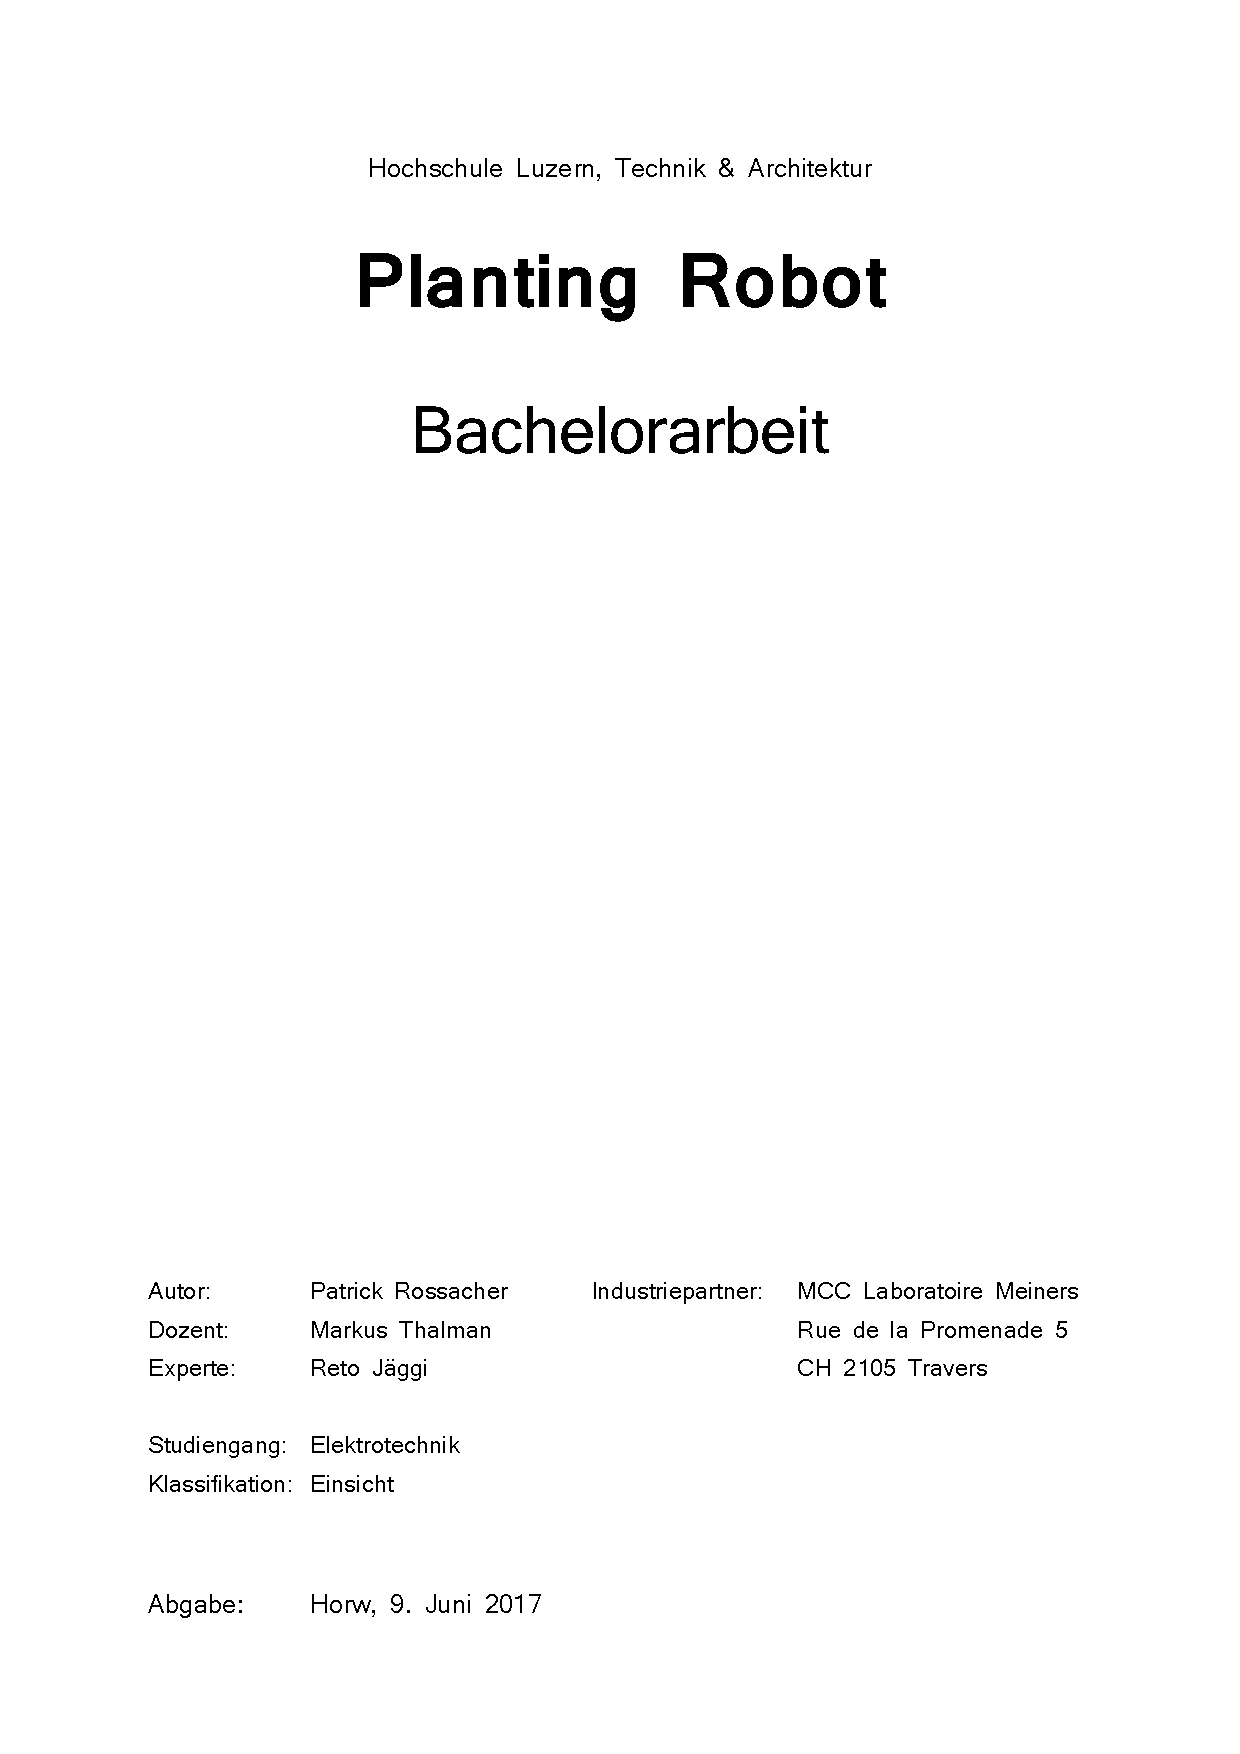
\includepdf{Illustrationen/0-Vorspann/Titelblatt.pdf}
\input{Kapitel/0_Vorspann/0.1_Redlichkeitserklärung}
\newpage
\fontsize{12}{15}
\selectfont
\sloppy
%\begin{sffamily}
\renewcommand{\contentsname}{Inhaltsverzeichnis}
\tableofcontents
%\end{sffamily}
\newpage
\begin{comment}
	\phantomsection\addcontentsline{toc}{section}{Abbildungsverzeichnis}

	\begin{sffamily}
	\listoffigures % Abbildungsverzeichnis
	\end{sffamily}	Inhalt...
\end{comment}

\begin{comment}
	\phantomsection\addcontentsline{toc}{section}{Tabellenverzeichnis} 
	\begin{sffamily}
	\newpage
	\listoftables % Tabellenverzeichnis
	\end{sffamily} 	Inhalt...
\end{comment}

\newpage
%\begin{sffamily}
\phantomsection\addcontentsline{toc}{section}{Glossar} 
\section*{Abkürzungsverzeichnis}\label{dok:glossar}
\begin{table}[H]
	\begin{tabular}{|L{2.5cm}|L{13cm}|}

		\hline	
		\textbf{ABS} & Acrylnitril-Butadien-Styrol. Thermoplast der in der Additiven Fertigung verwendet wird.\\
		
		\hline	
		\textbf{DC} & Direct Current\\

		\hline
		\textbf{FDM} & Fused Deposition Modeling. 3D-Druckverfahren: Kunststoff wird durch eine oder mehrere Düsen extrudiert und zu Bauteillagen zusammengeführt.\\
		
		\hline
		\textbf{GND} & Ground\\
		
		\hline
		\textbf{HSLU T\&A} & Hochschule Luzern für Technik und Architektur\\ 
		
		\hline
		\textbf{KDS} & Kinetis Design Studio\\

		\hline
		\textbf{LED} & Light-emitting diode\\
		
	 	\hline
	 	\textbf{PAIND} &  Industrieprojekt (Modul der HSLU) \\ 
	 	
	 	\hline
	 	\textbf{PCB} &	Printed Circuit Board\\
				
		\hline
		\textbf{RTOS} & Real Time Operating System \\
		
		\hline
		\textbf{SoC} &	System on Chip\\
		
		\hline
		\textbf{SWD} &	Serial Wire Debug\\
		
		\hline
		\textbf{UART} &	Universal Asynchronous Receiver Transmitter\\
		
		\hline
		\textbf{USB} &	Universal Serial Bus\\		
		
		\hline
		\textbf{openSDA} & Ein Seriell- und Debugadapter, welcher in diverse NXP Entwicklungsplatformen integriert ist.\\
		
		\hline
		\textbf{HMI} & Human Machine Interface\\
				
		\hline
	\end{tabular} 
	\vspace{0.2cm}
\end{table}


\subsection*{Begrifflichkeiten}
\begin{table}[H]
	
	\begin{tabular}{|L{4.5cm}|L{11cm}|}
		\hline
		\textbf{Adhäsion} & Adhäsion blabla.\\
		
		\hline
		\textbf{Batch} & Batch blabla.\\
		
		\hline
		\textbf{BLE} & Bluetooth Low Energy: Ein unter Bluetooth 4.0 eingeführter Standard zur Datenübertragung für portable Geräte.\\
		
		\hline
		\textbf{CAD} & Computer-aided Design: Rechnerbasierte Unterstützung von konstruktiven Aufgaben in der Produktentwicklung \\
		
		\hline		
		\textbf{Demonstrator PCB} & Eine im Umfang dieses Projekts entwickelte Printplatine.\\
		
		\hline		
		\textbf{Dockingstation PCB} & Eine im Umfang dieses Projekts entwickelte Printplatine.\\
		
		\hline		
		\textbf{FRDM-Board} & In diesem Projekt ist damit spezifisch das Freedom Board KL25Z gemeint. Ein Mikrocontroller Entwicklungsboard von NXP mit einem ARM Cortex-M0+ Prozessor. \\
		
		\hline
		\textbf{Hexiwear} & Ein Mikrocontroller Entwicklungsboard von NXP mit einem ARM Cortex-M0+ mit BLE (SoC) sowie einem ARM Cortex-M4 Prozessor und diversen Sensoren.\\
		
		\hline
		\textbf{Nut} & Nut blabla\\	
			
		\hline
		\textbf{Python} & Interpretierte Programmiersprache \\
		
		\hline		
		\textbf{Raspberry} & Raspberry Pi 3 Model B: Ein kompaktes Linux basiertes Computersystem mit einem Broadcom Quad Core Prozessor, 1GB RAM und Peripherie Schnittstellen. \\	
		
		\hline
		\textbf{RGB} &  Farbraum, welcher durch das mischen von rot, blau und grün eine Farbwahrnehmung nachbildet. \\
		
		\hline
		\textbf{MDF} &  Mitteldichte Faserplatte: Ein Holzwerkstoff bestehend aus feinstzerfasertem rindenfreiem Nadelholz, welches verpresst wird.  \\		
		
		\hline
		\textbf{NemaCaps} &  Das Setzgut des Planting Robots. Von der Firma MCC Laboratoire Meiners hergestellte Kapseln in Kugelform mit Nematoden als Inhalt. \\
		
		\hline
	\end{tabular} 
	\vspace{0.2cm}
\end{table}


%\end{sffamily}
\newpage
\pagenumbering{arabic}

\newpage
\section{Abstract}
\pagenumbering{arabic}
\textit{(ygu/pro)} Der Einsatz von Fadenwürmern zur Schädlingsbekämpfung in der Landwirtschaft, sowie im Gartenbau bietet eine biologische Alternative zu konventionellen Pestiziden. Die industrielle Bestückung von Töpfen mit Kapseln, welche Fadenwürmer beinhalten, birgt im Gartenbau einen hohen personellen Aufwand. Dieser Nachteil soll durch den Einsatz eines Pflanzroboters beseitigt werden. In einer interdisziplinären Gruppe wird  ein Funktionsmuster eines Roboters entwickelt, welches die automatische Dosierung, wie auch die Platzierung von Nematoden-Kapseln in Töpfen für den Gemüse- und Zierpflanzenbau ausführt. Dabei ist der Roboter an eine halbautomatische Topfmaschine gekoppelt.
\newline

Für die Entwicklung des Funktionsmusters wurde mittels Funktionsanalyse die Aufgabe funktional abstrahiert und in lösungsneutrale Teilfunktionen zerlegt. Die Ausarbeitung von drei Lösungskonzepten erfolgte durch die funktionsbezogene Variation von Teillösungen und einer Konzeptauswahl mittels morphologischem Kasten. Für eine verbesserte Einschätzung der Machbarkeit wurden kritische Teilfunktionen einem praktischen Funktionsnachweis unterzogen. Als Resultat der Nutzwertanalyse wurde eines der drei Konzepte für die Umsetzung ausgewählt.
\newline

Während der praktischen Umsetzung des Konzepts erfolgte die Entwicklung der Konstruktion, Software sowie der Elektronik in vermehrt fachspezifischer Arbeit. Die entwickelten Komponenten wurden hergestellt und als Gesamtsystem montiert. Abschliessend wurden Funktionstest an den einzelnen Einheiten durchgeführt.
\newline

Anhand des Funktionsmusters konnte aufgezeigt werden, dass eine industrielle Bestückung von NemaCaps realisitisch ist. Die Vereinzelung der Kapseln sowie die Konfiguration der Setzeinheit konnte durch das Funktionsmuster erfüllt werden. Weiter bleibt das Zusammenspiel aller Funktionen zu überprüfen, da eine umfassende Überprüfung innerhalb des gesetzten Zeitrahmen nicht realisierbar war.
\newline

Die gewonnenen Erkenntnisse aus den Funktionstests lassen vermuten, dass durch gezielte Anpassungen an der Setzeinheit die gestellte Aufgabe mit dem gewählten Konzept möglich ist. Für die abschliessende Umsetzung werden konkrete Massnahmen genannt.

\newpage
The application of nematodes for pest control in agriculture and gardening offers a biological alternative to conventional pesticides. The industrial assemby of pots with capsules which contain nematodes implies higher human resources in gardening than usual. This disadvantage is to be resolved by the application of a robot. In an interdisciplinary team, the development of a functional prototype of such a robot is to be undertaken which doses and places nematode-capsules in pots automatically. The pots are used for vegetable gardening and ornamental plants. The functional prototype is linked with a semi-automatic potting machine.
\newline

The development of this functional prototype was abstracted by a functional analysis. Furthermore an objective observation was undertaken and the main-function of the prototype was split into several sub-functions. Based on the functional analysis, an elaboration of three concepts was done by using creativity techniques and a morphological box. In order to support the assessment of those concepts, critical functions were tested. One of those concepts was chosen to be realised as a consequence of the utility analysis.
\newline

During the practial implementation of the chosen concept such as the design of the electronics, the software and the whole mechanical setup was carried out in mainly subject-specific tasks. The developed components were assembled and merged to a system. finally, the assembled components were undergone extensive testing procedures.
\newline

As conclusion the assembled functional prototype was shown to be able of handling NemaCaps. The separation of NemaCaps and configuration of the planting unit was tested successfully. An extensive examination of the  interaction between all functions could not be verified yet due to the lack of time.
\newline

The gained findings from testing the functional prototype lead to the supposition that an industrial assembly of NemaCaps with the chosen concept is likely. In order to finish the implementation thoroughly, specific measures are listed.

\newpage
\section{Methodik}

\newpage
\section{Einleitung}
\begin{wrapfigure}[16]{r}{8.5cm}
	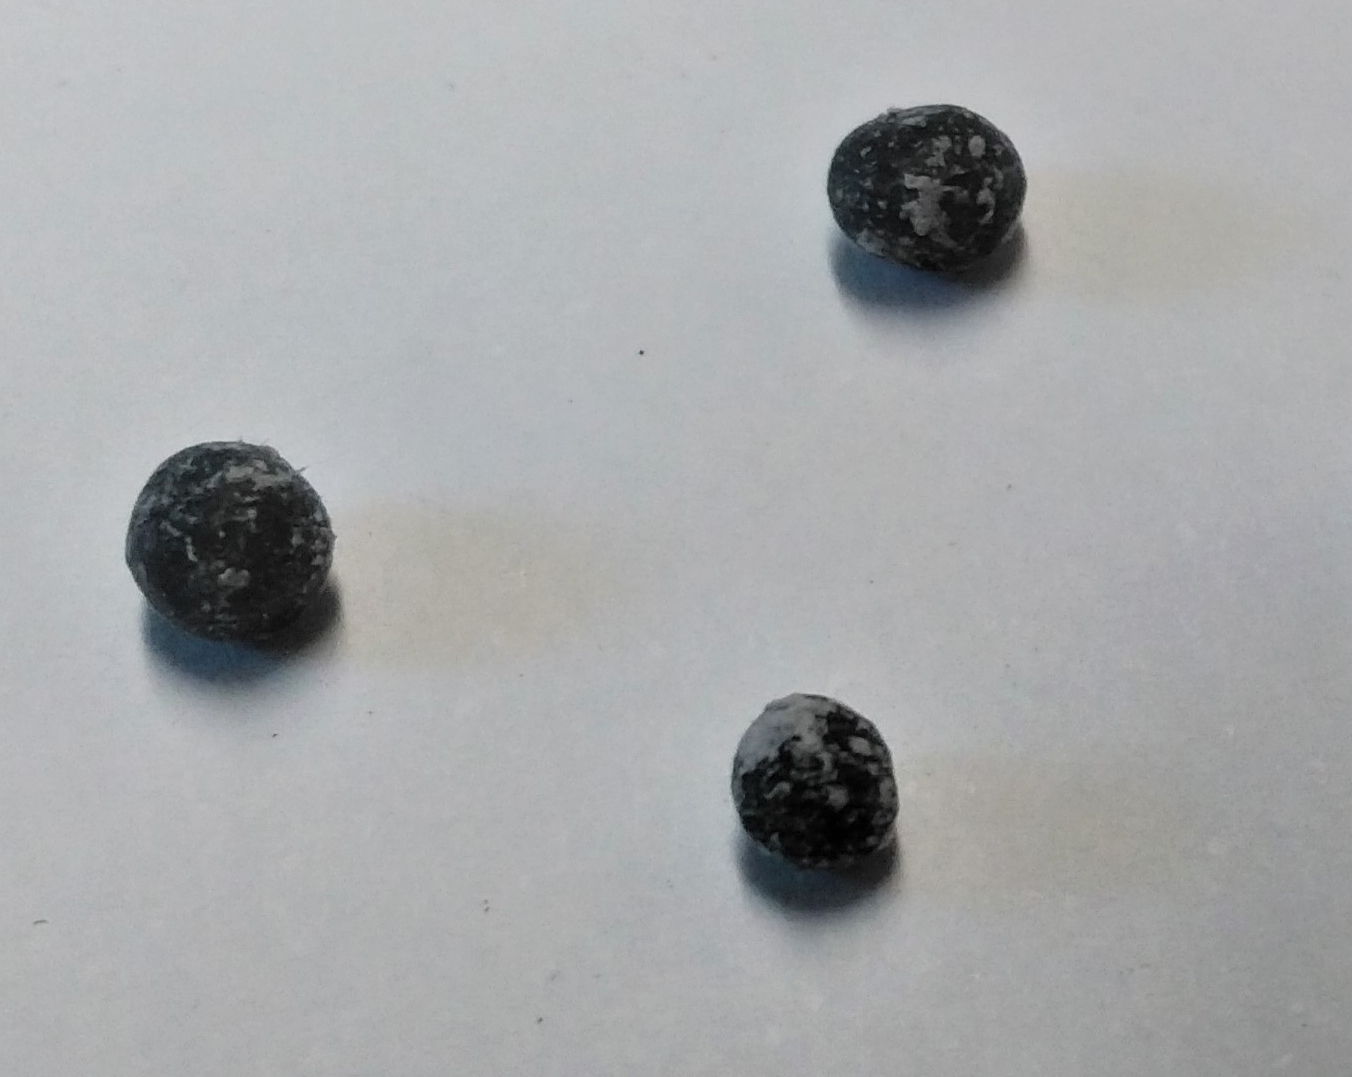
\includegraphics[scale=0.11]{Illustrationen/3-Einleitung/nemacaps.jpg}
	\caption{NemaCaps}
	\label{fig:nemacaps}
\end{wrapfigure}
Die Firma MCC Laboratoire Meiners GmbH ist in der Herstellung von Mikroverkapselungen tätig. Neben der Pharma- und Kosmetikbranche werden Mikroverkapselungen auch in der Landwirtschaft eingesetzt. Für diese Branche entwickelt MCC Laboratoire Meiners GmbH Kapseln, sogenannte NemaCaps, welche in der biologischen Schädlingsbekämpfung eingesetzt werden. Ein NemaCap beinhaltet mehrere tausend Fadenwürmer (Nematoden). Neben Nematoden ist der Kapsel ein Schlafmittel beigemischt, sodass die Fadenwürmer schlafend gestellt sind. 
\newline
NemaCaps werden im Erdreich eingesetzt. Im Wurzelbereich der zu schützenden Pflanze werden diese platziert. Durch das Begiessen der Pflanze oder Regenfall wird das Schlafmittel verdünnt und die Nematoden werden aktiv. Die Hülle der Kapseln besteht aus \textbf{\textit{XYZ}} welches elastische Eigenschaften besitzt. Dies ist Voraussetzung, dass die Nematoden nach dem Aufwachen die Kapsel durchbrechen können.\newline
In ihrer natürlichen Umgebung angelangt stossen die Fadenwürmer nun zufällig auf Larven von Schädlingen. Gemäss dem Nationalen Forschungsprogramm 68 [nachfolgend NFP 68]\cite{nfp} dringen die Nematoden durch die Körperöffnungen der Larven ein (Siehe Abb.  \ref{fig:zyklus_Nematoden}, Punkt 3). im Körper der Larve angelangt, setzen die Fadenwürmer dort Bakterien frei (Punkt 1 in Abb.  \ref{fig:zyklus_Nematoden}). Durch die rapide Vermehrung dieser Mikroben wird die Larve abgetötet. Im Innern der Larve vermehren sich nun die Nematoden bis diese komplett aufgezehrt ist \cite{nematoden}. Anschliessend verlassen die Nematoden den Kadaver und befallen weitere Larven. So beginnt der Kreislauf von Neuem (Punkt 2 in Abb.  \ref{fig:zyklus_Nematoden}).
\newline

\begin{wrapfigure}[10]{r}{7cm}
	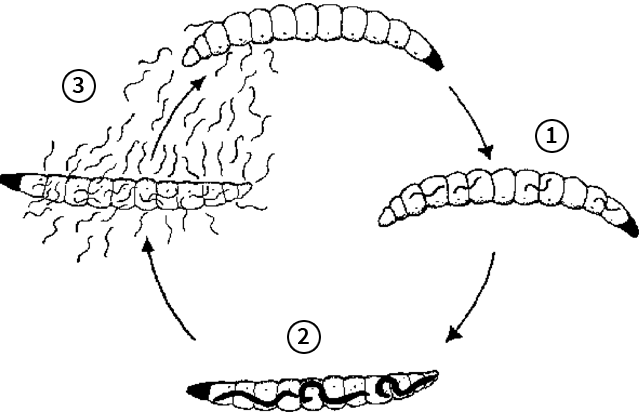
\includegraphics[scale=0.4]{Illustrationen/3-Einleitung/zyklus_nematoden.png}
\caption{Bekämpfung einer Larve durch Nematoden}
\label{fig:zyklus_Nematoden}
\end{wrapfigure}

	
Nematoden bieten speziell in der Bekämpfung gegen Wurzelschädlinge eine wirksame Alternative zu Pestiziden an. Pestizide können im Wurzelbereich weniger gezielt eingesetzt werden \cite{nfp}. Die Überlegenheit der Nematoden (im Wurzelbereich?) will man mit NemaCaps nutzen. Durch die Kapselung ist eine gezielte Platzierung sowie Dosierung von Nematoden möglich. Ein weiterer Vorteil der Kapselung ist die verbesserte Handhabung. Die einfache Lagerung sowie Transport von Fadenwürmer wird möglich.  Zusätzlich verlängert die Verwendung von Schlafmittel die Haltbarkeit der Nematoden. Diese Vorteile unterstreichen das Potential von NemaCaps, der biologischen Alternative von Pestiziden.

\newpage
\section{Einleitung}
Die Firma MCC Laboratoire Meiners GmbH ist in der Herstellung von Mikroverkapselungen tätig. Neben der Pharma- und Kosmetikbranche werden Mikroverkapselungen auch in der Landwirtschaft eingesetzt. Für diese Branche entwickelt MCC Laboratoire Meiners GmbH Kapseln, sogenannte NemaCaps, welche in der biologischen Schädlingsbekämpfung eingesetzt werden. Ein NemaCap beinhaltet mehrere tausend Fadenwürmer (Nematoden). Der Kapsel ist ein Schlafmittel beigemischt, sodass die Fadenwürmer schlafend gestellt sind. 
\begin{figure}[H]
	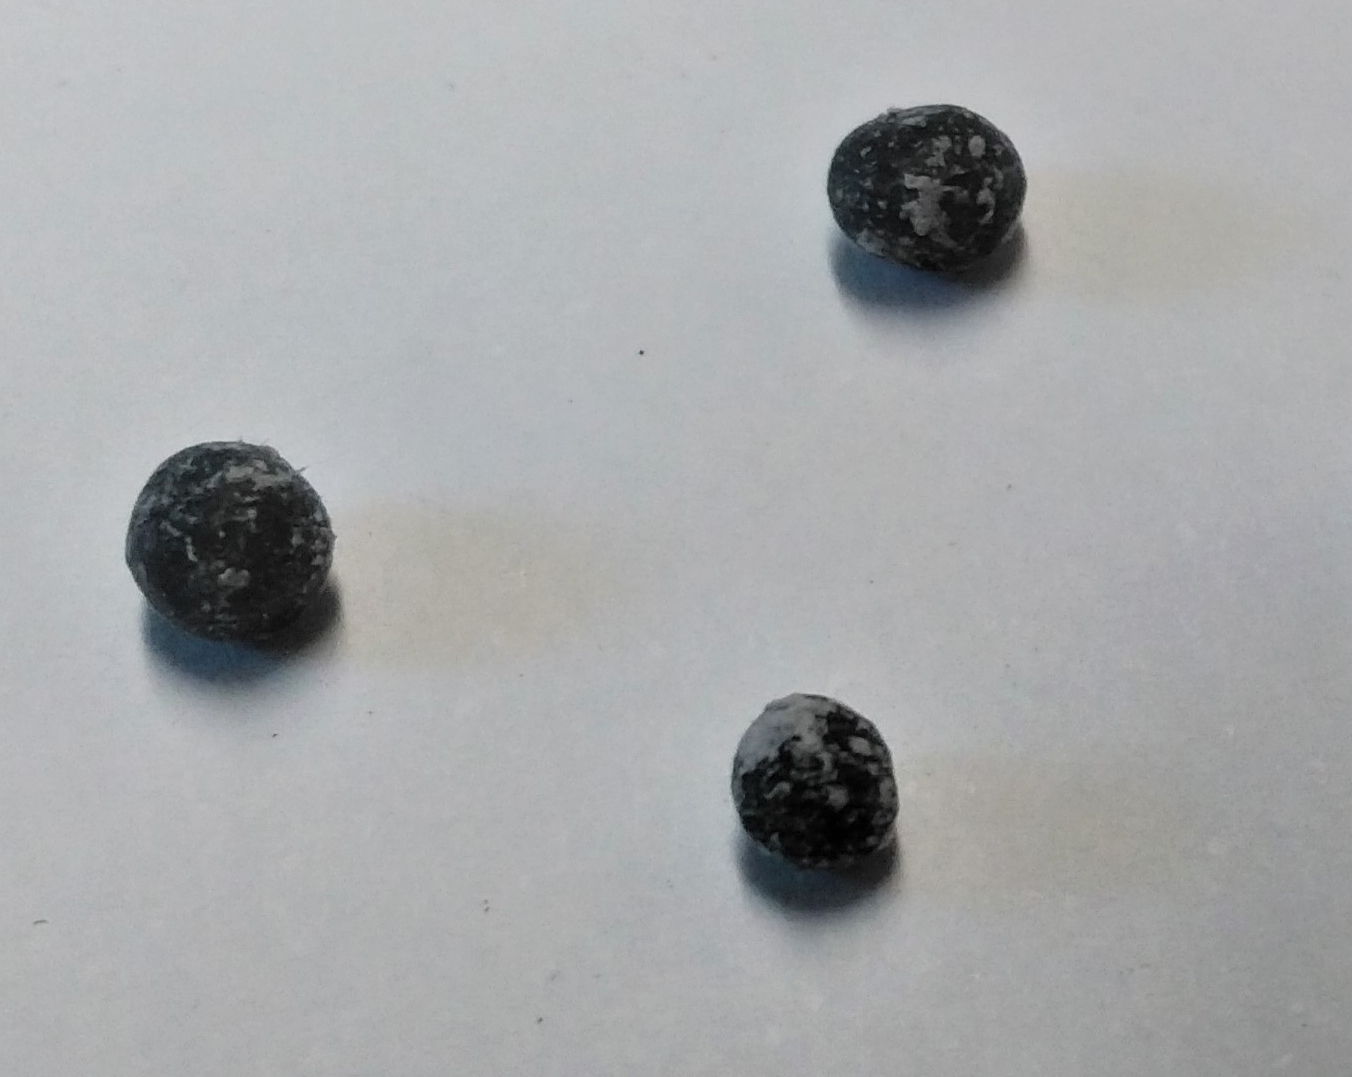
\includegraphics[width=1\textwidth]{Illustrationen/3-Einleitung/nemacaps.jpg}
	\caption{NemaCaps}
	\label{fig:nemacaps}
\end{figure}
NemaCaps werden im Erdreich eingesetzt. Im Wurzelbereich der zu schützenden Pflanze werden diese platziert. Durch das Begiessen der Pflanze oder Regenfall wird das Schlafmittel verdünnt und die Nematoden werden aktiv. Die Hülle der Kapseln besteht aus \textbf{\textit{XYZ}} welches elastische Eigenschaften besitzt. Dies ist Voraussetzung, dass die Nematoden nach dem Aufwachen die Kapsel durchbrechen können.\newline
In ihrer natürlichen Umgebung angelangt stossen die Fadenwürmer nun zufällig auf Larven von Schädlingen. Gemäss dem Nationalen Forschungsprogramm 68 [nachfolgend NFP 68] (2015) dringen die Nematoden durch die Körperöffnungen der Larven ein (Siehe Abb.  \ref{fig:zyklus_Nematoden}, Punkt 3). im Körper der Larve angelangt, setzen die Fadenwürmer dort Bakterien frei (Punkt 1 in Abb.  \ref{fig:zyklus_Nematoden}). Durch die rapide Vermehrung dieser Mikroben wird die Larve abgetötet. Nach Leillinger und Löckener (2012) vermehren sich die Nematoden im Innern der Larve bis diese komplett aufgezehrt ist. Nun verlassen die Nematoden den Kadaver und befallen weitere Larven. So beginnt der Kreislauf erneut von vorne (Punkt 2 in Abb.  \ref{fig:zyklus_Nematoden}).\newline
\begin{figure}[H]
	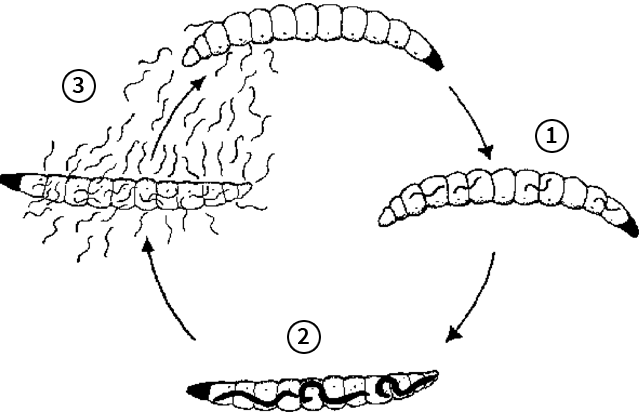
\includegraphics[width=1\textwidth]{Illustrationen/3-Einleitung/zyklus_nematoden.png}
	\caption{Bekämpfung einer Larve durch Nematoden}
	\label{fig:zyklus_Nematoden}
\end{figure}
	
Nach dem NFP 68 (2015) bieten Nematoden speziell in der Bekämpfung gegen Wurzelschädlinge eine wirksame und sichere Alternative zu Pestiziden an, welche im Wurzelbereich weniger gezielt eingesetzt werden können. Dadurch werden die Vorteile der NemaCaps gegenüber von Pestiziden deutlich. Nematoden können im Wurzelbereich gezielt platziert sowie dosiert werden. Ein Vorteil der Kapselung ist die verbesserte Handhabung. Die einfache Lagerung sowie Transport von Fadenwürmer wird möglich.  Zusätzlich wird durch die Verwendung des Schlafmittels die Haltbarkeit der Nematoden verlängert. Diese Vorteile unterstreichen das Potential von NemaCaps, der biologischen Alternative von Pestiziden.

\subsection{Ausgangslage}
Der Einsatz von Nematoden ist im Gartenbau verbreitet. Konventionell werden Nematoden gemäss Birchmeier (\textbf{\textit{2017}}) in Wasser aufgelöst und durch ein Dosiergerät oder eine Spritzkanne in Pflanzennähe aufgetragen. Solche Produkte werden jedoch erst bei erhöhtem Befall von Schädlingen eingesetzt. Der Ansatz der Firma MCC Laboratoire Meiners GmbH ist jedoch ein Anderer. Präventiv möchten Sie Nematoden in Topfpflanzen einsetzen. Im Detailhandel sollen so Topfpflanzen - bereits bestückt mit NemaCaps - im Verkauf angeboten werden.
\newline
Die industrielle Anwendung von NemaCaps birgt bei manueller Bestückung von Töpfen einen hohen personellen Aufwand. 
\subsection{Aufgabenstellung}
MCC Laboratoire Meiners GmbH möchte ihr Produkt (NemaCaps) während der halbautomatischen Bestückung von Topfpflanzen in den Töpfen platzieren. Nach der Beschüttung der Erde (Punkt 2 in Abbildung \ref{fig:schema_topfmaschine}) sollen NemaCaps im Wurzelbereich der Pflanze platziert werden. Die manuelle Bestückung von NemaCaps würde einen zusätzlichen personellen Aufwand bedeuten. Ob Gartenbauunternehmen bereit sind diesen aufzuwenden, darf hinterfragt werden. Um den Einsatz von NemaCaps lukrativer zu gestalten, möchte MCC Laboratoire Meiners GmbH ein automatisiertes System (besser Roboter?) entwickeln, welcher die Bestückung der NemaCaps ausführt (übernimmt?). Dabei soll dieses System auch in der Lage sein, verschiedene Topfgrössen zu handhaben.
\newline

Diese Bachelorarbeit befasst sich mit der Entwicklung eines Funktionsmusters, welche die automatische Bestückung von NemaCaps an einer Topfmaschine übernimmt. Dieses Funktionsmuster soll eine greifbare Vorstellung vermitteln, wie die industrielle Implementierung dieser Automatisationsaufgabe aussehen kann. 
\newline 

Die Aufgabenstellung beinhaltet:
\begin{itemize}
	\item \textbf{Ausarbeitung eines Pflichtenhefts:} Am Anfang vom Entwicklungsprozess steht eine genaue Analyse der Aufgabenstellung. In Zusammenarbeit mit MCC Laboratoire Meiners GmbH soll der Umfang der Bachelorarbeit abgegrenzt werden. Produkteigenschaften, Anforderungen an das Funktionsmuster und Randbedingungen (gegeben durch Topfmaschine, Töpfe und Topferde) stehen dabei im Fokus. Am Ende dieser Phase soll ein detailliertes Pflichtenheft entstehen.
	 
	\item \textbf{Konzeptausarbeitung und Entscheid:} Auf das Pflichtenheft folgt die interdisziplinäre Ausarbeitung von Lösungsvarianten. Durch eine sorgfältige Auslegung aller Vor- und Nachteile der ausgearbeiteten Lösungsvarianten soll die Beste Lösungsvariante ausgeweählt werden. Wichtig ist dabei, dass durch die funktionelle Abstraktion der Aufgabe eine lösungsneutrale Betrachtung möglich wird. Erst dies schafft die Grundlage für einen kreativen Lösungsfindungsprozess und gewährleistet eine volle Auschöpfung des Potenzials dieser Phase. Am Ende dieser Phase, und nach einer objektiven Beurteilung aller Lösungsvarianten, soll ein Entscheid stehen, welches der ausgewählten Lösungsvarianten umgesetzt wird.
	
	\item \textbf{Funktionsnachweis krtischer Funktionen:} Teillösungen, die als kritisch erachtet werden, sind einem praktischen Funktionsnachweis zu unterziehen. Die Erkenntnisse des Funktionsnachweises sollen unterstützend in die Beurteilung der Lösungskonzepte einfliessen und den Entscheid stützen.
	
	\item \textbf{Realisation eines Funktionsmusters:} In der Implementationphase soll das ausgearbeitete Konzept als Funktionsmuster realisiert werden. In dieser Phase werden fachspezifisch die einzelnen Komponenten hergestellt und getestet. (Mehr nötig?)
	
	\item \textbf{Erstellung eines Projektplans:} Die gewünschte Realisation eines Funktionsmusters erfordert einen klar definierten Zeitplan. Darin sollen auch Lieferfristen und der erforderliche Zeitbedarf von Fertigungsverfahren mitberücksichtigt werden. Auch sollen Reservezeiten eingeplant werden, falls allfällige Verzögerungen eintretten. Optional (Idealerweise?) wird dieser Projektplan von einer Risikoanalyse begleitet (unterstützt?).
	
	\item \textbf{Dokumentation:} Eine umfassende schriftliche Dokumentation über die methodische Vorgehensweise sowie aller relevanten technischen Überlegungen ist zu verfassen. 
	
\end{itemize}

\newpage
\section{Entwurf}
\textit{(pro)} Dieses Kapitel soll einen Überblick über die Rahmenbedingungen sowie die Anforderungen an den Planting Robot bieten. Ausführlichen Angaben zu diesen Themen sind im Pflichtenheft (siehe Anhang) formuliert. Basierend auf dem Pflichtenheft wurde ein abstrakter Entwurf des Planting Robots in Form einer Funktionsanalyse erstellt. Der Inhalt dieses Kapitels resultiert aus der Zusammenarbeit mit der Firma MCC Laboratoire Meiners, dem Topfmaschinenhersteller Leidolt Maschinenbau sowie den betreuenden Dozenten dieses Projektes.

\subsection{Rahmenbedingungen}
Die in diesem Unterkapitel beschriebenen Rahmenbedingungen sollen die Aufgabenstellung präzisieren und auf den Umgang mit den in diesem Projekt verwendeten Materialien aus dem Agrar-Bereich sensibilisieren.

\subsubsection{NemaCaps}
Die geometrischen Abmessungen der NemaCaps sind entscheidend, da sie während des Setzprozesses vereinzelt und transportiert werden müssen. Die Abmessungen der NemaCaps wurden deshalb vom Hersteller MCC Laboratoire Meiners mit 3mm Durchmesser und einer Toleranz von +0.6mm spezifiziert. Von Bedeutung ist ausserdem das Alter und die Lagerung der Nemacaps. Sie müssen in einem geschlossenen Gefäss, unter Beigabe eines hygrophoben Pulvers bei unter 7°C gelagert werden. Dabei sollten sie zur Zeit der Verwendung nicht älter als 4 Wochen sein. NemaCaps welche längere Zeit der Umgebungsluft ausgesetzt waren, schrumpfen um ein Vielfaches ihrer ursprünglichen Grösse.

\begin{figure}[H]
	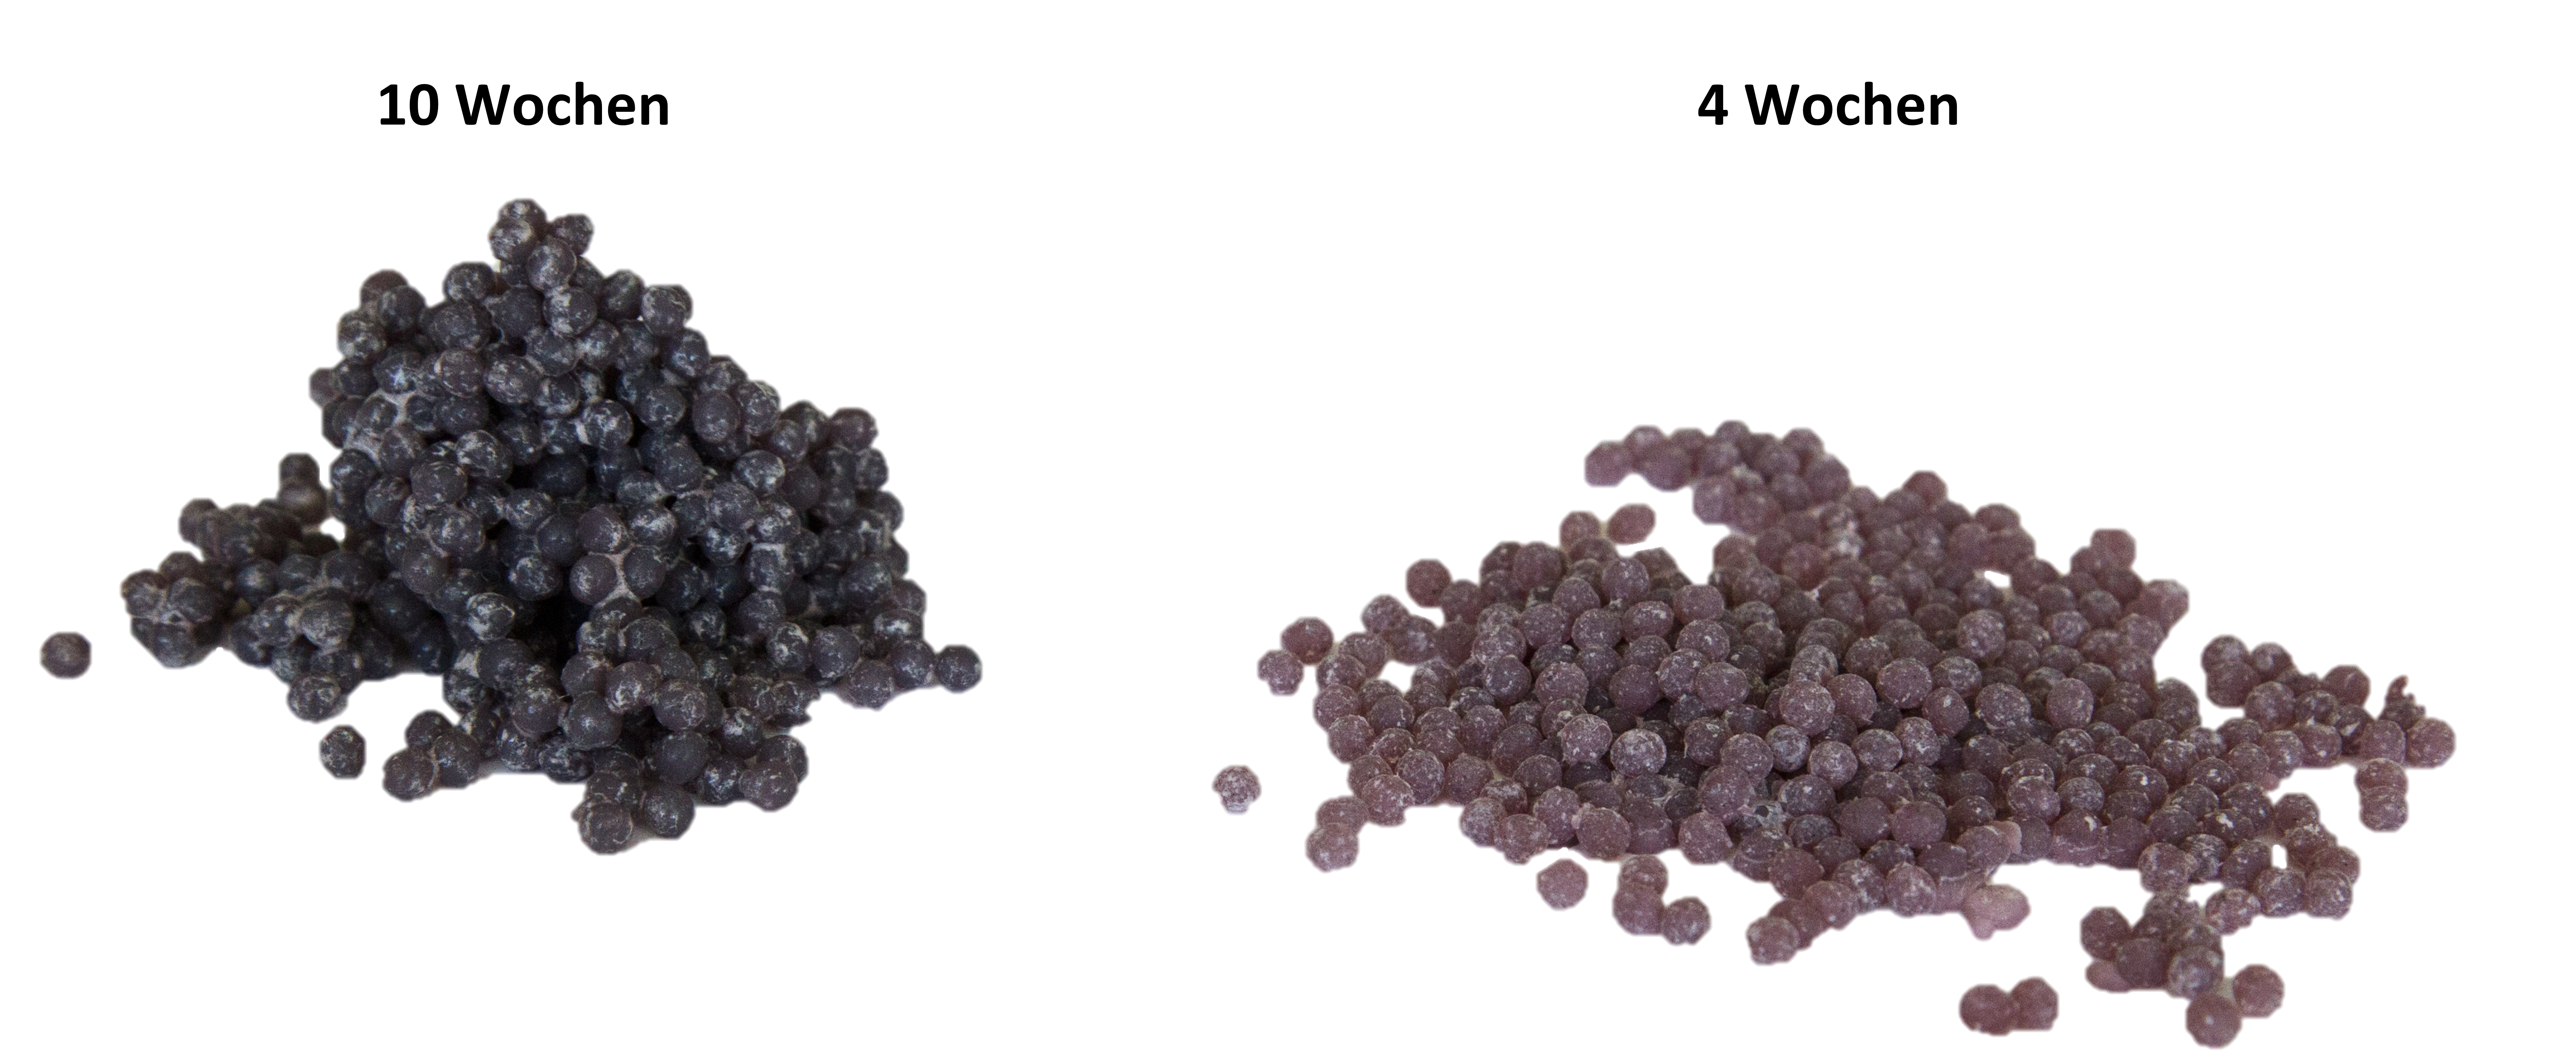
\includegraphics[draft=false,width=1\textwidth]{Illustrationen/4-Entwurf/nemacaps_altvsneu_1.jpg}
	\caption{NemaCaps bei korrekter Lagerung mit einem Alter von 10 bzw. 4 Wochen}
	\label{fig:nemacaps_altvsneu}
\end{figure}

In Abb. \ref{fig:nemacaps_altvsneu} ist der Unterschied zwischen NemaCaps welche 10 Wochen bzw. 4 Wochen alt sind, an der Farbe deutlich zu erkennen. Diese NemaCaps wurden unter korrekten Bedingungen gelagert. Dies veranschaulicht deutlich, dass nur frische NemaCaps zu Testzwecken verwendet werden sollten. Die Konsistenz der 10 Wochen alten NemaCaps ist deutlich klebriger. Diese lassen sich zu Klumpen formen und sind nur schwer vereinzelbar.

\subsubsection{Töpfe und Topferde}
Sie liegen im Fokus des Planting Robots, kleine zylindrische Container der Firma Pöppelmann, auch Blumentöpfe genannt. Um einen genauen Anhaltspunkt für die Realisierung des Setzprozesses sowie der Topferkennung zu haben, wurden die zu bestückenden Töpfe definiert. So werden zu Testzwecken ausschliesslich Töpfe des Typs VCD9, VCD11, VCD12, VCD13 und VCD14 verwendet. Abb. \ref{fig:toepfe} zeigt einen Topf des Types VCD15.

\begin{figure}[H]
	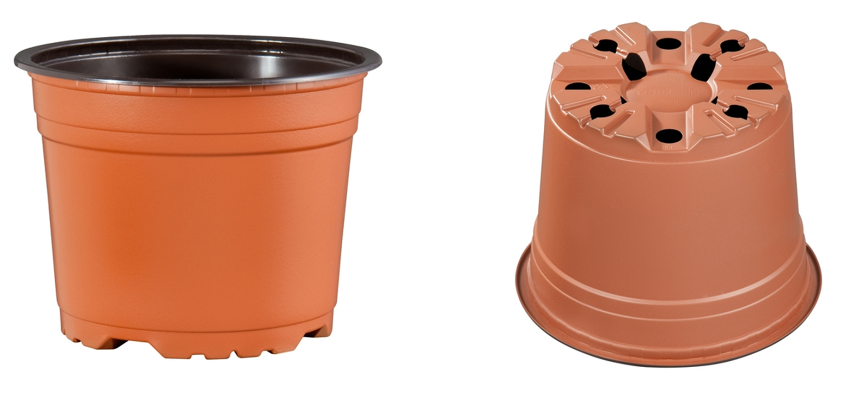
\includegraphics[draft=false,width=0.7\textwidth]{Illustrationen/4-Entwurf/VCD_Serie.png}
	\caption{Pöppelmann VCD Serie \protect\cite{Poeppelmann}}
	\label{fig:toepfe}
\end{figure}

Von substanzieller Bedeutung ist auch die verwendete Pflanzenerde. Da Erde von minderer Qualität eine hohe Menge an Fremdkörper wie Gehölz und Lehm enthalten kann. Die im Zusammenhang mit diesem Projekt verwendete Topferde ist deshalb auf die Artikel Nr.: 181 000 00 vom Hersteller RICOTER spezifiziert.

\subsection{Anforderungen}
Die in diesem Unterkapitel ausgehandelten Anforderungen an den Planting Robot dienen zur Abgrenzung des Funktionsumfangs des Projekts. Weiter sollen sie dem Industriepartner eine genaue Vorstellung darüber bieten, was er von dem fertigen Funktionsmuster erwarten kann.\\
\newline
Der Planting Robot soll stationär, auf dem Boden, neben der Topfmaschine platziert werden. Um einen präzisen Eingriff in die Produktionskette der Topfmaschine gewährleisten zu können, soll er an der Topfmaschine fixiert werden können. Der Planting Robot muss direkt am Topfkranz positioniert werden. Weiter soll der Planting Robot mit 230V Netzspannung ohne weitere Anschlüsse (z.B. Pressluft) betrieben werden können. Da der Planting Robot ein Funktionsmuster darstellt soll er nur für räumlichen Umgebungsbedingungen ausgelegt werden. \\
\newline
Der Setzprozess soll nur ausgeführt werden, wenn sich ein Topf in Position befindet. Drei Nemacaps sollen in einem Kreis mit einem Radius von 60$\%$ der Topfgrösse, mit einem Winkelabstand von jeweils 120°, in den Topf eingesetzt werden (siehe Abb. \ref{fig:Setzprozess}). Dabei soll die Einsetztiefe variabel verstellbar sein, aber maximal 60$\%$ der Topfhöhe betragen. 

\begin{figure}[H]
	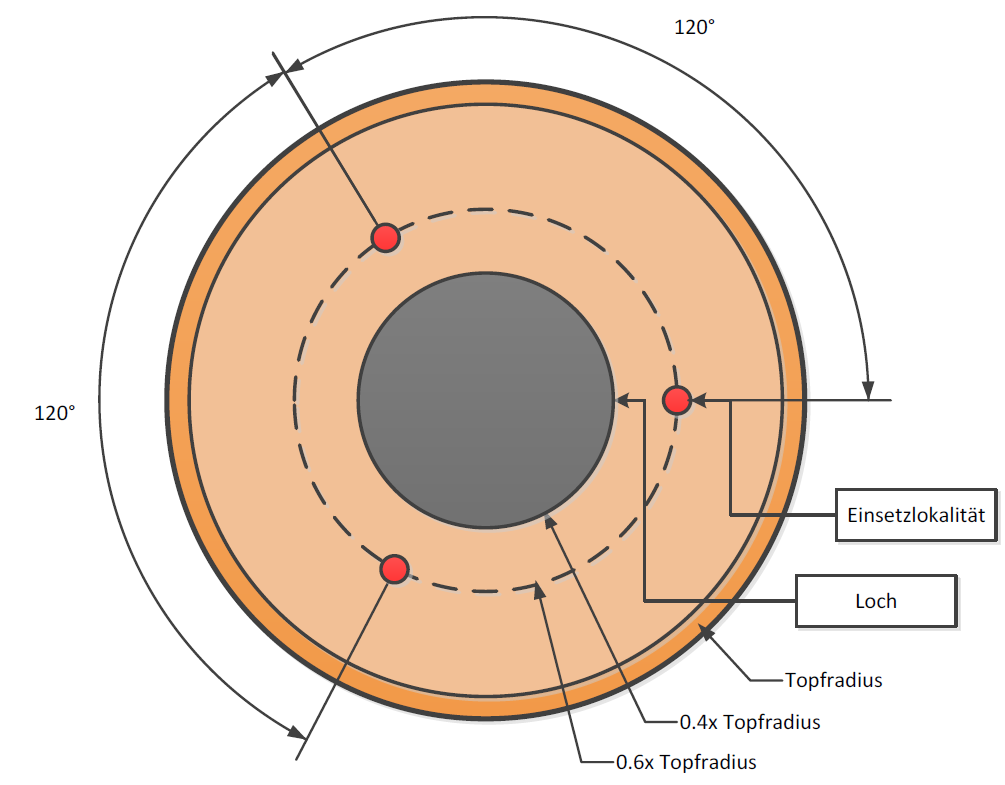
\includegraphics[draft=false,width=0.8\textwidth]{Illustrationen/4-Entwurf/Setzprozess.png}
	\caption{Setzlokalität}
	\label{fig:Setzprozess}
\end{figure}

Während eines Produktionsbatches soll sich die Topfgrösse nicht ändern. Beim Wechsel auf einen neuen Batch mit anderer Topfgrösse soll der Planting Robot umkonfiguriert werden. Eine Wunschanforderung ist es, dass sich der Planting Robot automatisch auf einen Wechsel der Topfgrösse konfiguriert. Die Setzkadenz des Planting Robots soll mit der normalen Betriebsgeschwindigkeit der Topfmaschine TC2 mithalten können. Demnach sollen 2800 Töpfe pro Stunde mit Nemacaps bestückt werden können. Wunschanforderung ist eine Produktionskapazität von 3600 Töpfen pro Stunde. Dabei ist zu beachten, dass die Eingriffszeit des Planting Robots aufgrund der Stopp- and Go-Bewegung des Topfkranzes nur 50$\%$ beträgt.
\subsection{Funktionsanalyse}

In diesem Kapitel wird der Planting Robot in verschieden Funktionsblöcke zerlegt. Die dadurch definierten Teilfunktionen ermöglichen ein systematisches Maschinendesign. Zu den jeweiligen Funktionsblöcken werden in Kapitel \ref{kap:Teilkonzept} verschiedene Lösungsvarianten ausgearbeitet. Diese Teilkonzepte werden anschliessend in Kapitel \ref{kap:LoesungsKonzept} zu einem kompletten Maschinendesign zusammengeführt.\newline
Bei der Funktionsanalyse wird zwischen einer Pflicht und einer komplexeren Wunschanforderung unterschieden. Die Wunschanforderung beschreibt zusätzlich zum vollen Funktionsumfang, eine selbstständig Konfiguration des Planting Robots auf verschieden Topfgrössen.


\begin{figure}[H]
	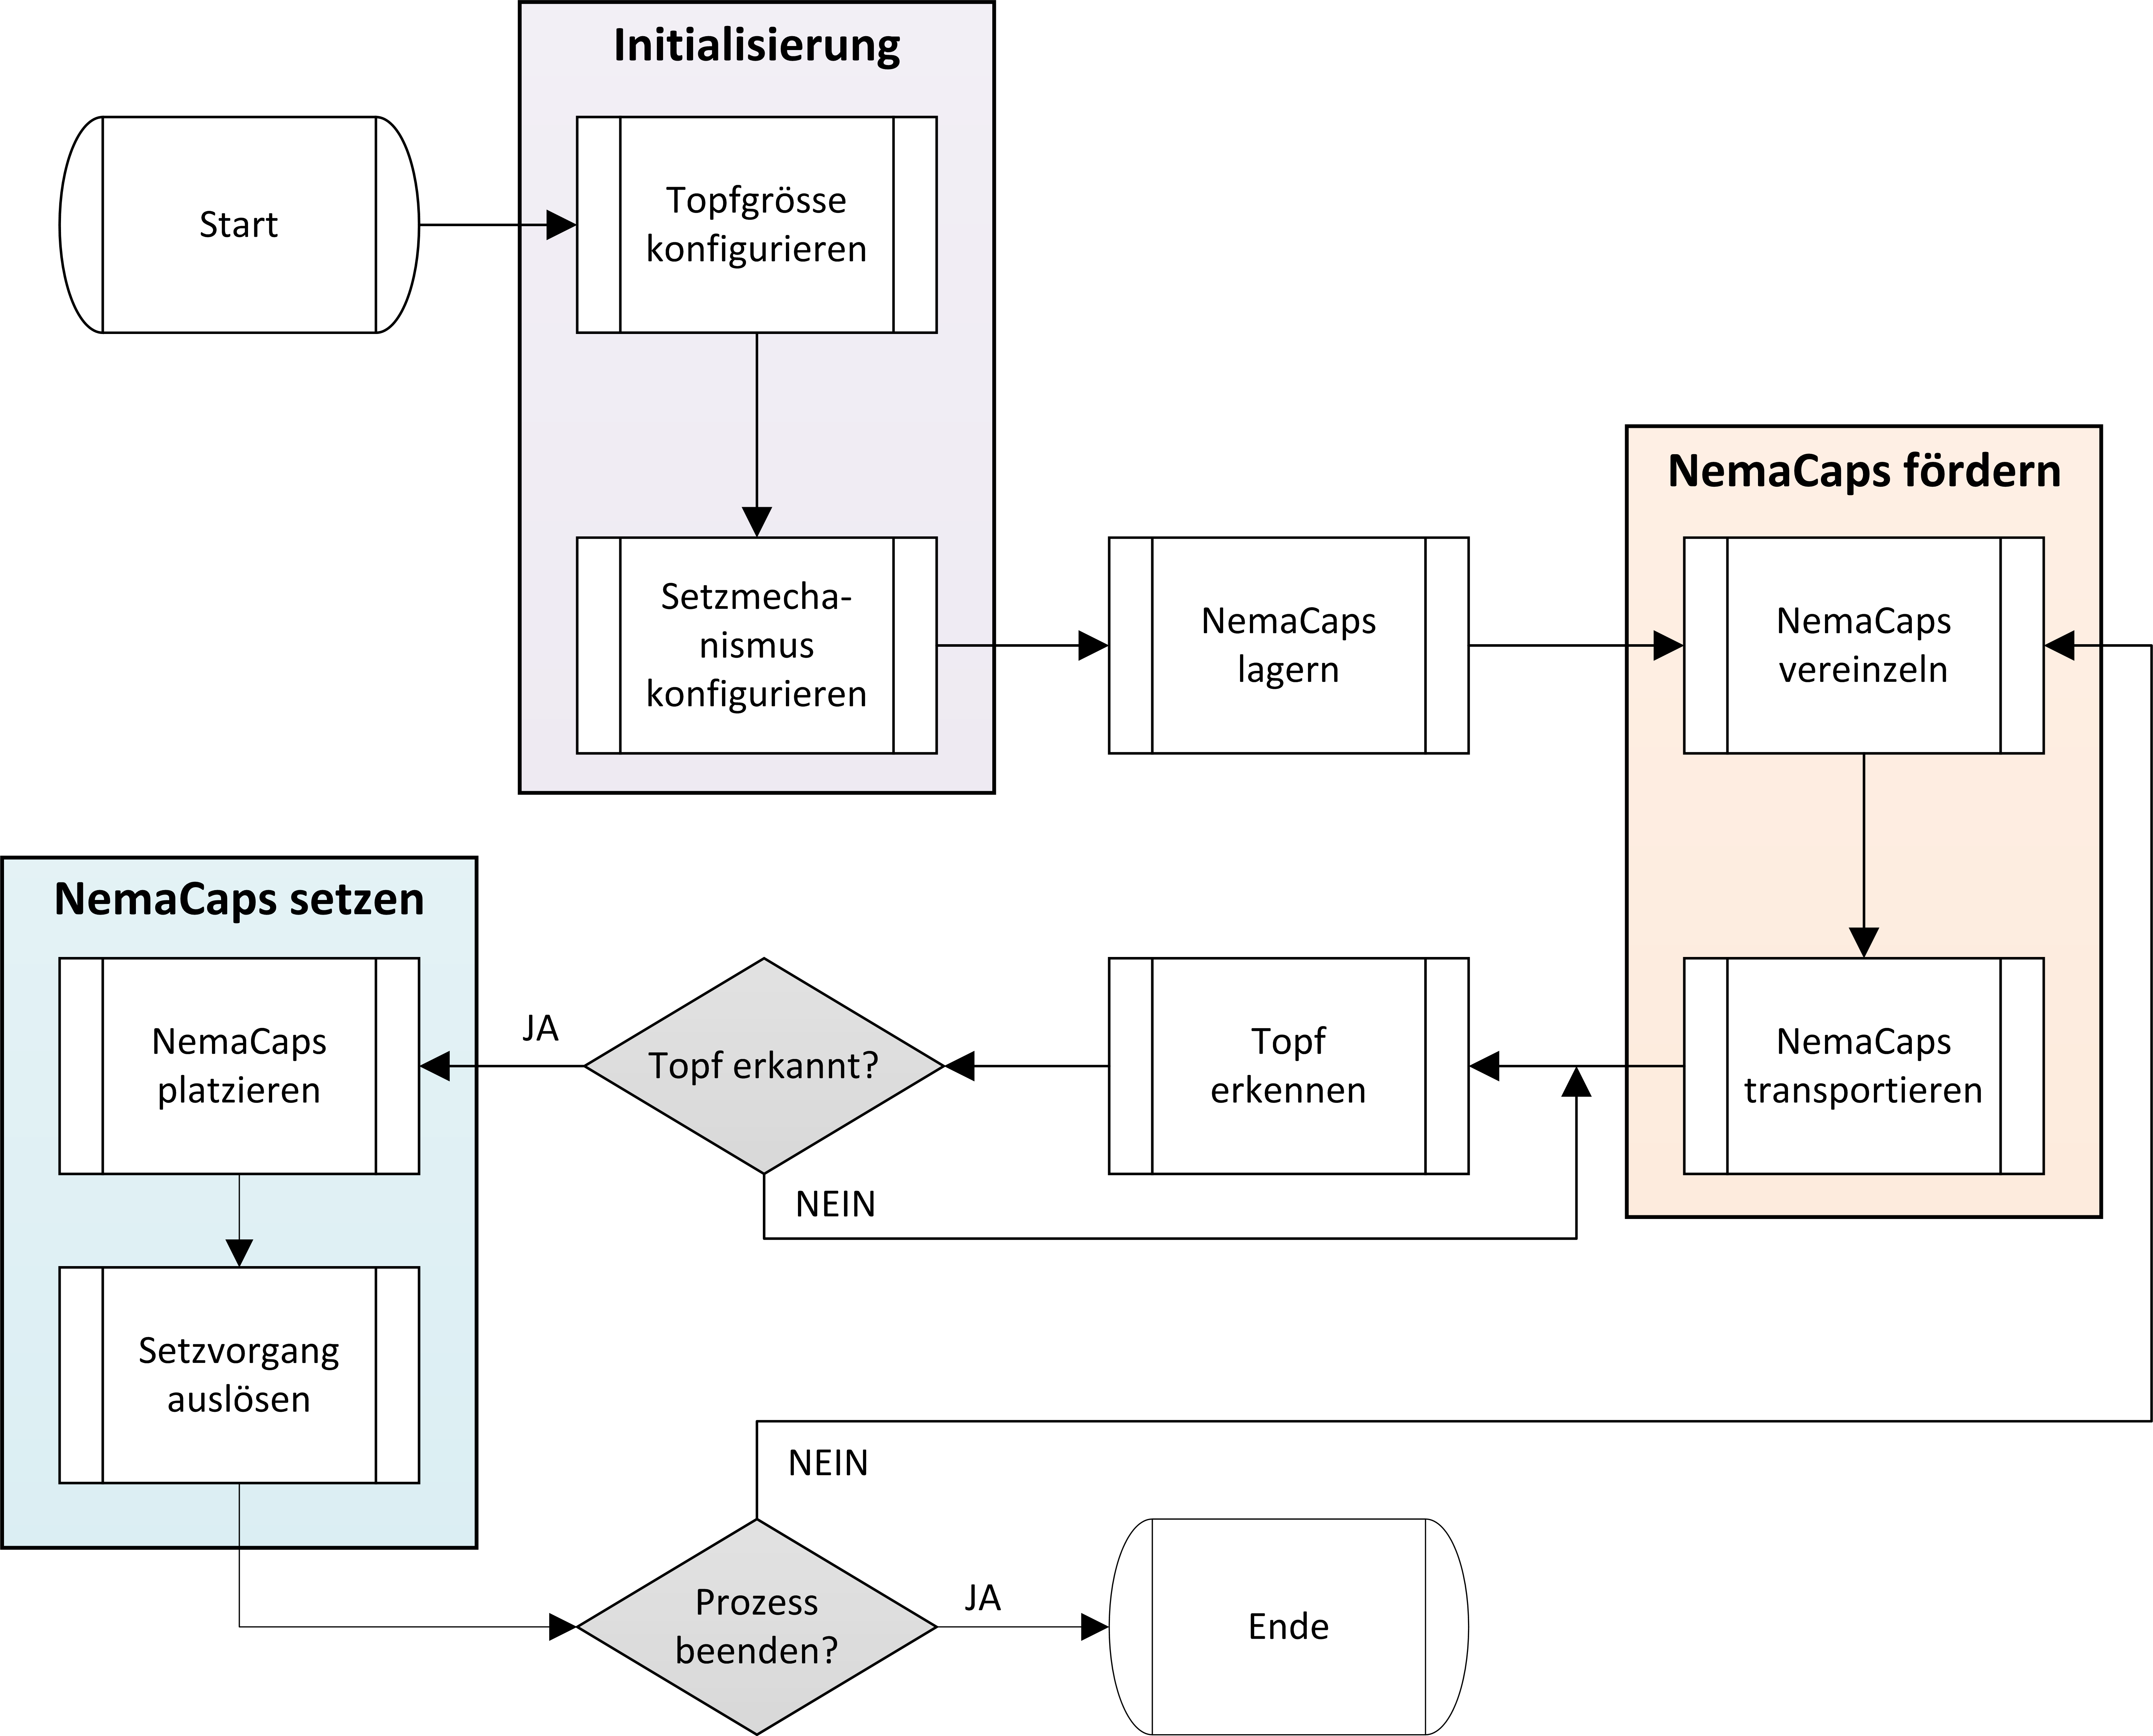
\includegraphics[width=1\textwidth]{Illustrationen/4-Entwurf/Funktionsanalyse_Pflicht.png}
	\caption{Funktionsanalyse Pflicht Blockdiagramm}
	\label{fig:FunktPflicht}
\end{figure}

\begin{itemize}
	\item \textbf{Initialisierung:} Die Initialisierung wird von einem Operator ausgeführt. Dieser Block ist nur in der Pflichtanforderung vorhanden, da die Maschine im Umfang der Pflichtanforderung die Initialisierung nicht selbstständig durchführt.
	
	\begin{itemize}
		\item \textbf{Topfgrösse konfigurieren:} In diesem Funktionsblock wird an der Maschine über ein HMI die verwendete Topfgrösse eingestellt.

		\item \textbf{Setzmechanismus konfigurieren:} Der Setzmechanismus muss für verschiedene Topfgrössen eingestellt oder ausgetauscht werden.
	\end{itemize}
	
	\item \textbf{NemaCaps lagern:} Das Setzgut (NemaCaps) wird in der Maschine mit einem Bestand von bis zu 10'000 Einheiten gelagert.
	
	\begin{figure}[H]
		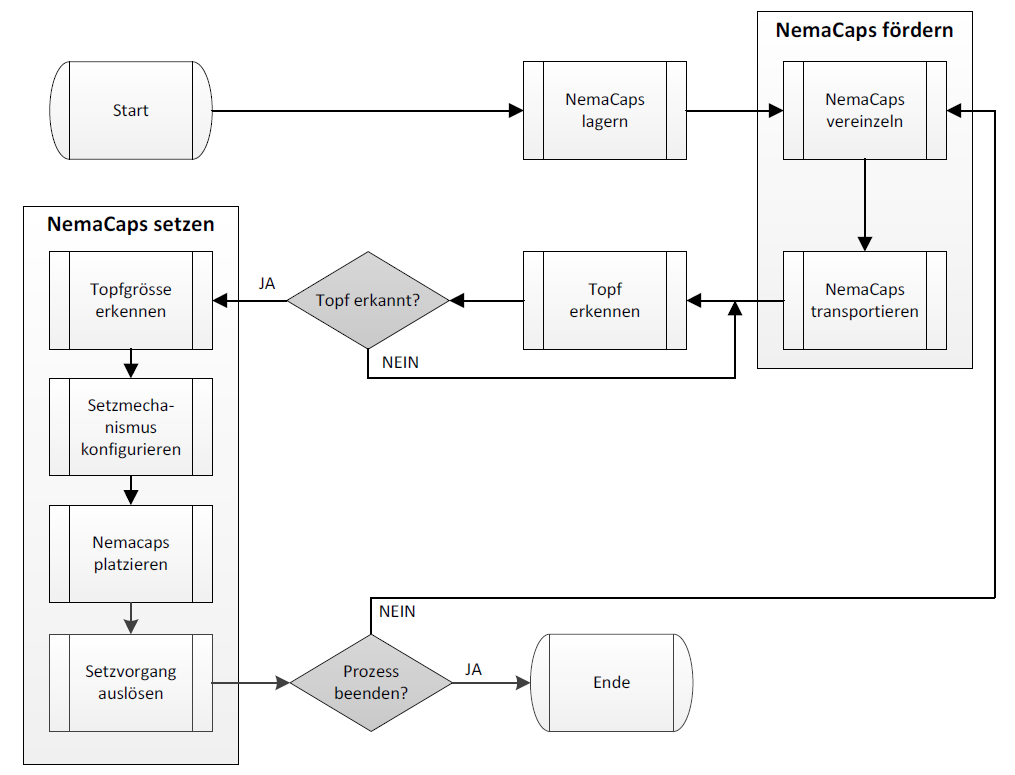
\includegraphics[width=1\textwidth]{Illustrationen/4-Entwurf/Funktionsanalyse_Wunsch.png}
		\caption{Funktionsanalyse Wunsch Blockdiagramm}
		\label{fig:FunktWunsch}
	\end{figure}
	
	\item \textbf{NemaCaps fördern:} Dieser Block behandelt die Verbindung zwischen Lager und Setzmechanismus.
	
	\begin{itemize}
		\item \textbf{NemaCaps vereinzeln:} Um die NemaCaps gezielt und kontrolliert in die Topferde einsetzen zu können, sollen diese vor dem Setzen vereinzelt werden.
		
		\item \textbf{NemaCaps transportieren:} Der Transport zwischen Lager und Setzmechanismus kann vor oder nach der Vereinzelung stattfinden.
	\end{itemize}




	\item \textbf{Topf erkennen:} Dieser Block übernimmt implizit zwei Aufgaben. Es soll erkannt werden ob überhaupt ein Topf für den Setzprozess bereit steht und ob sich dieser bewegt oder still steht. 
	
	\item \textbf{NemaCaps setzen:} Erst wenn ein Topf bereit steht wird der Setzprozess eingeleitet. Dieser unterscheidet sich wie in Abb. \ref{fig:FunktPflicht} und Abb. \ref{fig:FunktWunsch} ersichtlich zwischen Pflicht und Wunschanforderung anhand des Funktionsumfangs.
	
	\begin{itemize}
		\item \textbf{Topfgrösse erkennen:} Durch Sensorik soll die Topfgrösse jedes Topfes vermessen werden.
		
		\item \textbf{Setzmechanismus konfigurieren:} Anhand der gewonnen Daten zur Topfgrösse, soll die Maschine den Setzmechanismus selbstständig adaptieren.
		
		\item \textbf{Nemacaps platzieren:} Es folgt der eigentliche Setzprozess, in welchem die Nemacaps in einer definierten Anordnung in Position gebracht werden.
		
		\item \textbf{Setzvorgang auslösen:} Die Nemacaps welche vorher in Position gebracht wurden, werden nun in diesem Schritt vom Setzmechanismus in die Erde befördert.
	\end{itemize}
	
\end{itemize}

\subsection{Funktionsbezogene Variation}
\subsection{Technologierecherche}

\input{Kapitel/5_Konzept/5.1_Lösungskonzepte}
\subsection{Funktionsnachweis kritischer Funktionen}
Dieses Unterkapitel befasst sich mit dem praktischen Nachweis von kritischen Teilfunktionen. Kritische Teilfunktionen sind Funktionen, welche bei einem Ausfall dieser Teilfunktion, einen Ausfall des Gesamtsystems zur Folge hat. Dabei soll die Umsetzung einfacher Funktionsmuster einen praktischen Nachweis bringen, ob die Umsetzung von dieser Teillösung realistisch ist. Diese Beurteilung wird für Bewertung der ausgearbeiteten Lösungskonzepte miteinbegezogen.
\newline
Bei Betrachtung der Funktionsanalysen (Abbildungen \ref{fig:FunktPflicht} und \ref{fig:FunktWunsch}) ist erkennbar, dass beide Varianten (Pflicht sowie Wunsch) eine Serieschaltung darstellen. Bei einer Umsetzung einer Maschine mit einfacher Redundanz ergibt dies implizit, dass jede Funktion als kritisch eingestuft werden kann. Aus zeitlichen Gründen kann ein umfassenden Nachweis von allen Teillösungskonzepten nicht abschliessend durchgeführt werden. Eine pragmatische Auswahl von Funktionen mit erhöhtem Ausfallrisiko und einer vielversprechenden Funktionserfüllung wird daher angestrebt.

\subsubsection{NemaCaps vereinzeln und fördern}
Die Vereinzelung sowie Förderung von Gütern ist in der Automatisationsbranche ein bedeutendes Thema. Die automatisierte Sortierung sowie Transport eines Gutes sind grundlegende Bedingungen, sodass ein Produkt überhaupt in der automatisierten Serienfertigung herstellbar wird. Da solche Lösungen vielfach beide Funktionen miteinander vereinen, werden diese gemeinsam in einem Unterkapitel untersucht.
\newline
\newline
\textbf{Vibrationswendelförderer}
\newline
Ein Gerät das die Verzeinzelung sowie Förderung von Werkstücken vereint ist der Vibrationswendelförderer. Mittels Schwingungsenergie wird eine Wanderbewegung der Werkstücke erzeugt, welche beim Passieren von Schikanen vereinzelt werden. Weitere Erklärungen zum Wendelförderer sind im \textbf{Anhang} zu entnehmen.
\newline
Aus vergangenen Studentenarbeiten besitzt die Hochschule Luzern für Technik und Architektur einen solchen Wendelförderer. Dimensioniert ist dieser für die Vereinzelung von gezuckerten Mandeln. Auch wenn dadurch die Vereinzelung nur bedingt funktionsfähig ist, eignet sich dieses Gerät zur ersten Überprüfung der Funktion mit NemaCaps. 

Praktische Tests mit NemaCaps konnten am 15.3.2017 am Wendelförderer durchgeführt werden. NemaCaps wurden ins Haufwerk (Punkt 1 in Abbildung \ref{fig:wendelfoerderer}) eingefüllt und der Wendelförderer gestartet. Durch die Vibration sammelten sich die NemaCaps im Wendel (2) und begannen zu wandern. Die Förderung klappte einwandfrei, wobei die rasche Transportgeschwindigkeit positiv überraschte. 
\begin{figure}[H]
	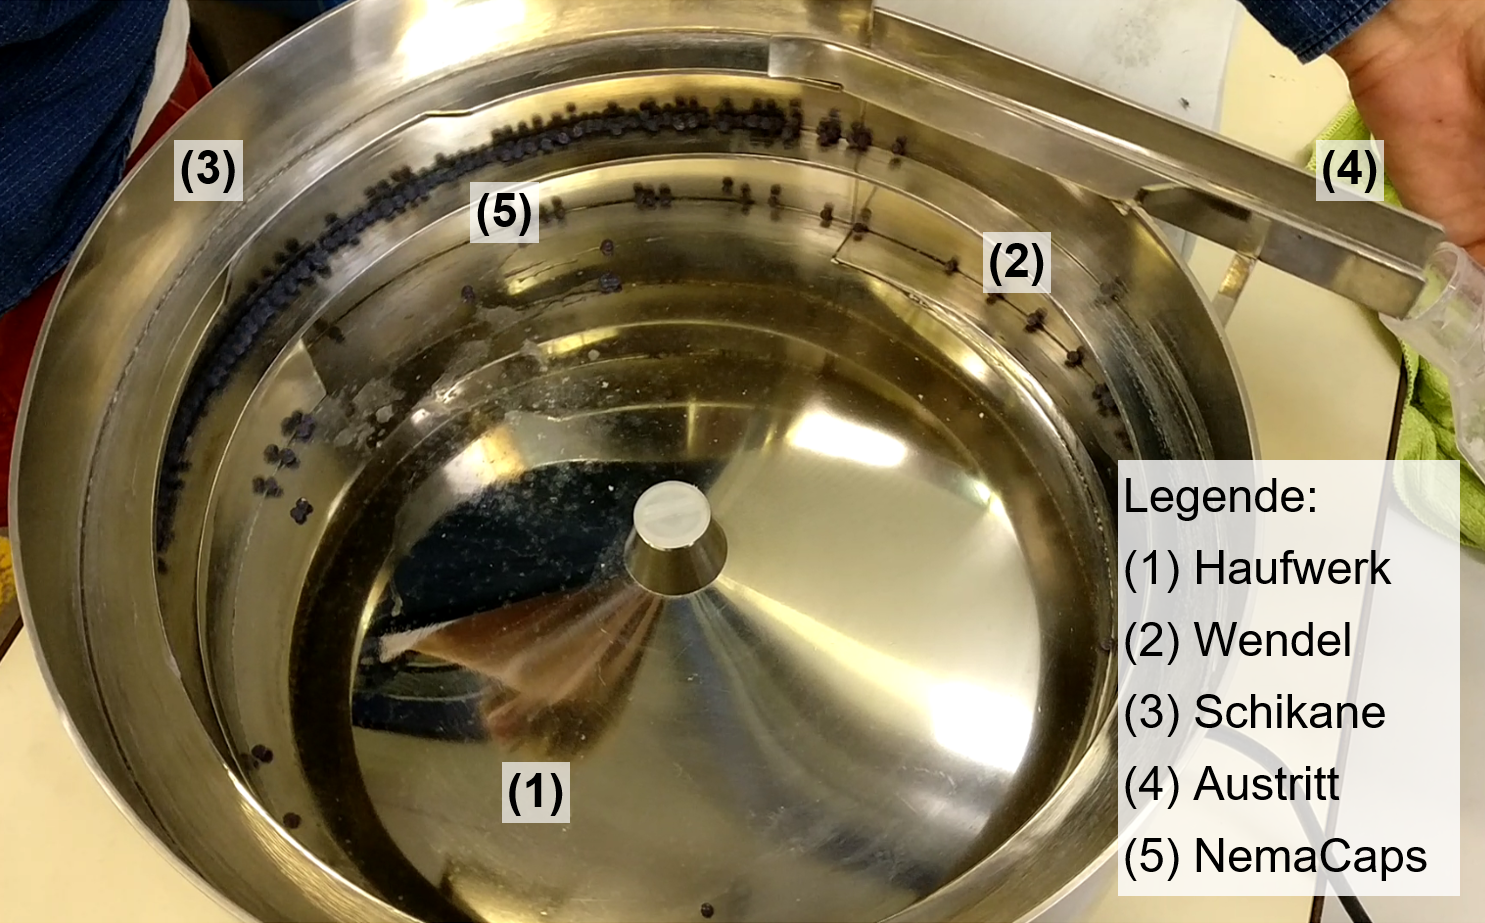
\includegraphics[width=1\textwidth]{Illustrationen/5-Konzept/wendelfoerderer.PNG}
	\caption{Praktische Tests am Wendelförderer der Hochschule}
	\label{fig:wendelfoerderer}
\end{figure}
\textbf{Erkenntnisse}
\newline
Folgende Erkenntnisse lieferten die Versuche:
\begin{itemize}
	\item Eine Förderung von NemaCaps mit einem Wendelförderer ist möglich. Die NemaCaps eignen sich als Fördergut und werden mit einer hohen Zuverlässigkeit gefördert.
	
	\item Die Schikane erfüllt ihre Funktion nicht. Dies ist allein auf die Tatsache zurückzuführen, dass der verwendete  Wendelförderer für gezuckerte Mandeln dimensioniert wurde. Eine Anpassung der Schikanen auf NemaCaps ist technisch machbar und ist kein Hindernis.
	
	\item Die Umsetzung der Funktionen NemaCaps vereinzeln und fördern mit einem Wendelförderer ist aus rein technischer Sicht realisierbar.
\end{itemize} 
\newpage
\textbf{Rotierende Lochmaske}
\newline
\begin{wrapfigure}[26]{r}{10cm}
	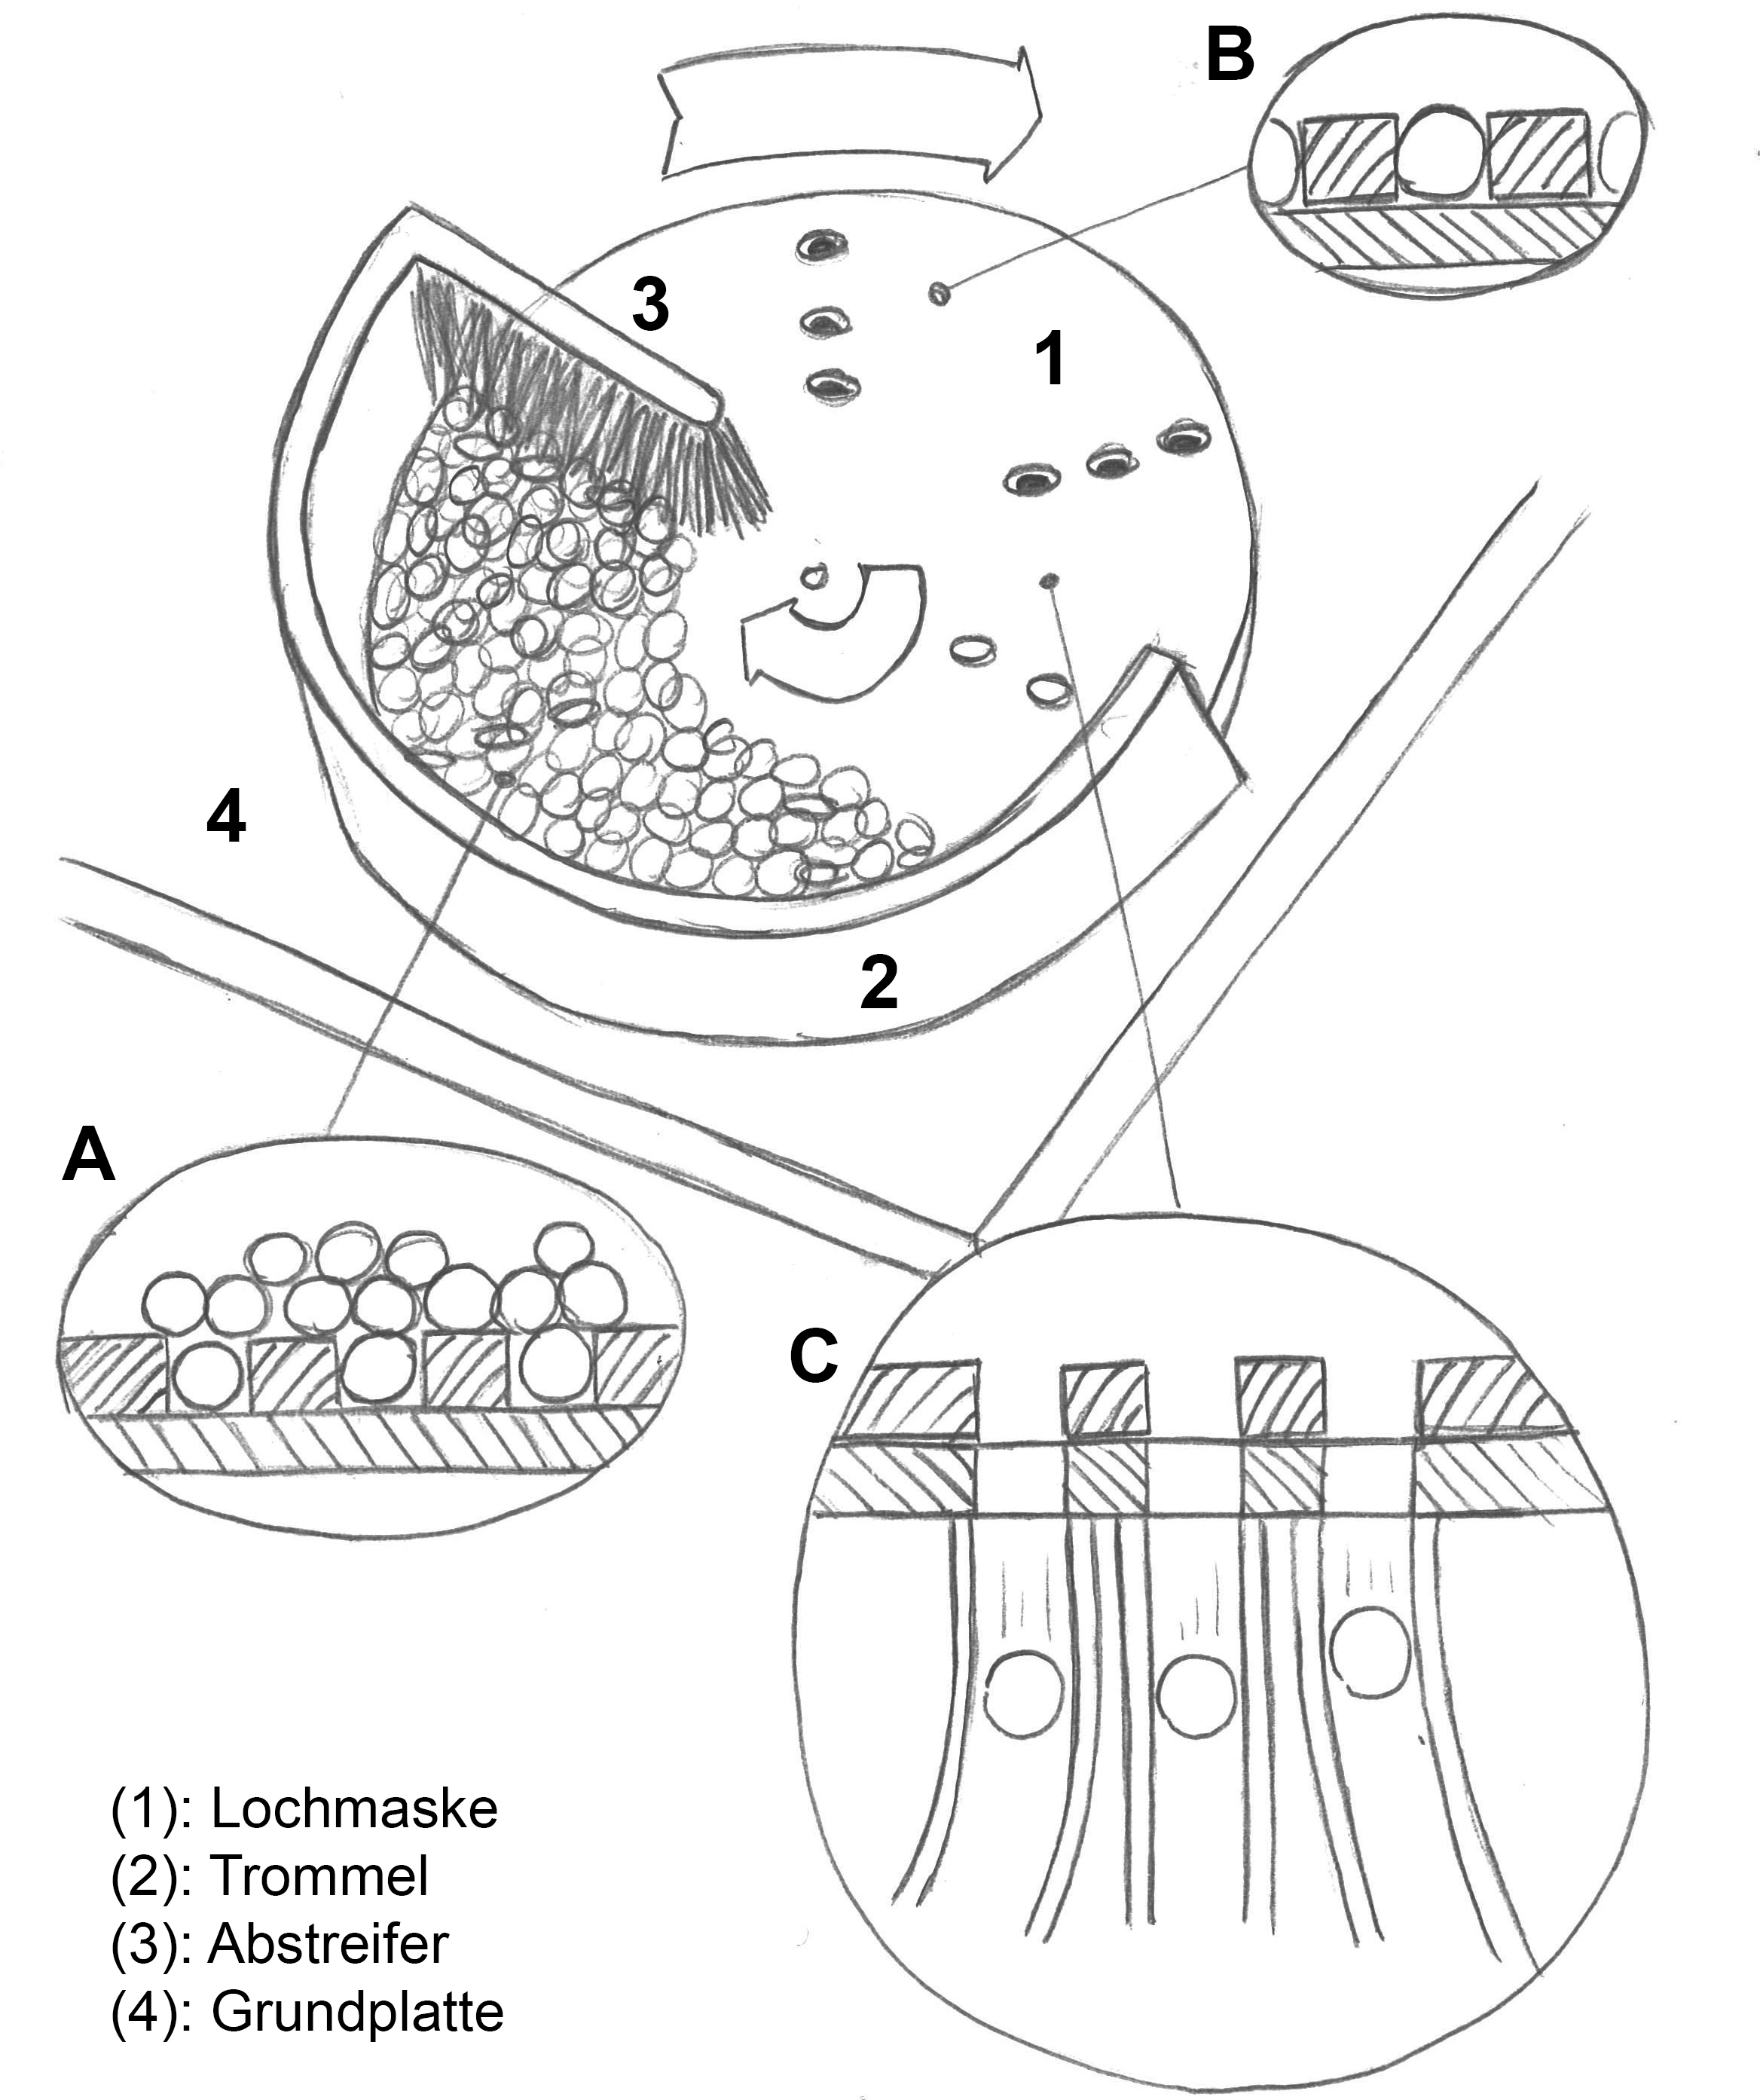
\includegraphics[scale=0.52]{Illustrationen/5-Konzept/schema_vereinzelung.jpg}
	\caption{Vereinzelung durch rotierende Lochmaske}
	\label{fig:schema_vereinzelung}
\end{wrapfigure}
Ein weiteres Konzept ist die Vereinzelung durch eine rotierende Lochmaske. Dabei werden die NemaCaps in einen Behälter gefüllt (Punkt 2 in Abbildung \ref{fig:schema_vereinzelung}). Im Behälter befindet sich eine rotierend gelagerte Scheibe mit Löchern (Lochmaske, 1). Die Löcher sind so gross, dass gerade ein NemaCap darin Platz hat. Durch die Rotation der Lochmaske fallen nun NemaCaps in die Maske (Detail A) und werden zu Detail B transportiert. Ein Abstreifer (hier in Form einer Bürste) sorgt dafür, dass überschüssige NemaCaps zurückgehalten werden. In der Grundplatte (4) sind Löcher vorgesehen, sodass bei Detail C die NemaCaps in Schläuche fallen. Idealerweise wird dieser Aufbau schief gelagert. 
\newline
\newline
Dieses Konzept wird von der Firma Kofatec GmbH für die Vereinzelung von Pfefferkörner eingesetzt. Dabei ist das Design des Funktionsnachweises stark am Funktionsmuster der Firma Kofatec GmbH angelehnt. Das Funktionsmuster wird mittels Lasermaschine aus MDF hergestellt. Auch wird die Lochmaske für den Funktionsnachweis von Hand betrieben.
\newline
Am 21.3.2017 wurde am umgesetzten Funktionsmuster der Funktionsnachweis erbracht. Durch zielgerichtetes Ausprobieren von verschiedenen Durchmesser der Löcher wurde die Lochmaske für die NemaCaps ausgelegt. Dann wurde mittels manuellem Rotieren die Vereinzelung überprüft.
\newline
\newline
Folgende Erkenntnisse lieferten die Versuche:
\begin{itemize}
	\item Die Lochmaske nimmt zuverlässig NemaCaps auf. Auch ein Transport zur Auslösung (Detail C in \ref{fig:schema_vereinzelung}) verläuft problemlos.
	
	\item Die Abstreifung von NemaCaps funktioniert. Kritisch ist dabei die Wahl des Abstreifers. Verwendet man zu scharfkantige Gegenstände kann es passieren, dass ein NemaCap verschnitten wird. Weiter wurde erkannt, dass NemaCaps heikel auf Scherbeanspruchungen reagieren. Dies Eigenschaft ist nicht zu unterschätzen.
		
	\item Die Zuverlässigkeit der Auslösung am Punkt C ist durchschnittlich. Dies wird damit erklärt, dass nicht frische NemaCaps verwendet wurden. Dadurch hat sich das hygroskope Pulver in Wasser gewandelt und so die Adhäsion der NemaCaps erhöht. Dadurch blieben geschätzte 50 Prozent der NemaCaps an der Lochmaske hängen. Auch ist ein holzfaserbasiertes Material für die Lochmaske ungeeignet. Die rauhe Oberfläche der Bohrung bietet so mehr Haftung.
	
	\item Durch leichtes Antippen der Grundplatte oder einem Luftstoss konnten alle NemaCaps ausgelöst werden. Dies zeigt, dass durch Abhilfemassnahmen durchaus eine höhere Zuverlässigkeit erreicht wird.
	
	\item Die Umsetzung von diesem Lösungsansatz ist nur realistisch, wenn klare Abhilfemassnahmen und Verbesserungen der Lochmaske zur Steigerung der Zuverlässigkeit definiert werden. 
\end{itemize} 
\textbf{Bild des Funktionstests?}

\subsubsection{NemaCaps setzen}
Ein Lösungsansatz der Teilfunktion "NemaCaps setzen" basiert auf der Idee zuerst ein Loch auszuheben oder zu verdrängen und dann ein NemaCap ins Loch fallen zu lassen. Ähnlich ist eine andere Idee, welche mit einer spitzen Zange das Loch verdrängt wird, sich die Zange in der Erde öffnet und so ein NemaCap platziert.
\newline
Um die Umsetzbarkeit dieser Ideen zu überprüfen, werden zwei Versuche durchgeführt:
\begin{itemize}
	\item \textbf{A) Ermittlung der Verdrängkraft:} Mit einer konventionellen Setzhilfe aus dem Gartenbau werden praktische Tests durchgeführt. Dabei wird ein Topf mit dem vorgegebenen Gartenhumus von Ricoter befüllt und leicht angepresst. Nun wird die maximale Einsetztiefe an der Setzhilfe markiert und schrittweise mit Gewicht (Masse m in Abbildung \ref{fig:skizze_setzversuch}) beschwert. Sobald die Markierung den Gartenhumus berührt, wird die Setzhilfe inklusive Masse m gewogen und durch die Multiplikation mit der Erdbeschleunigung die benötigte Verdrängkraft ermittelt.
	
	\item \textbf{B) NemaCap mittels Zange setzen:} Der identische Versuch wird mit der genannten Zange durchgeführt. Zusätzlich wird in die geschlossene Zange ein NemaCap gegeben. Bei Erreichung der Setztiefe wird die Zange geöffnet und das NemaCap platziert. Realisiert wird die Zange aus gelasertem MDF.
\end{itemize} 

\begin{figure}[H]
	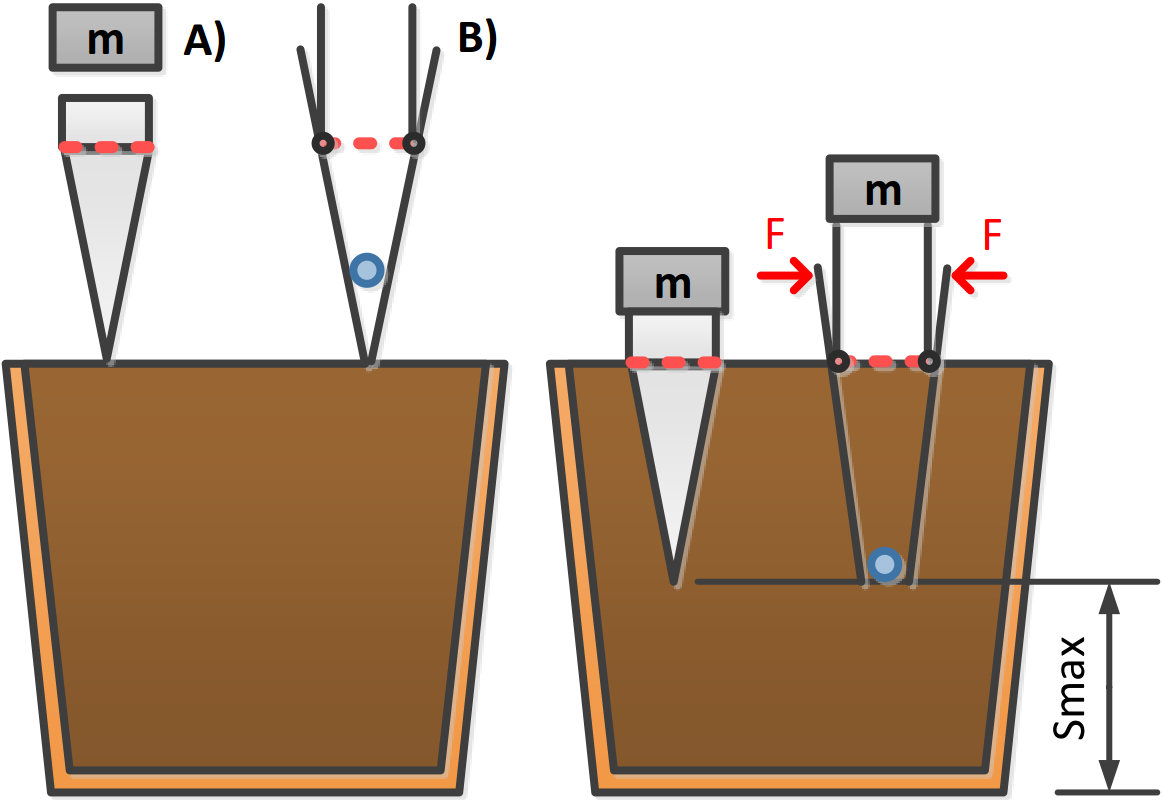
\includegraphics[width=1\textwidth]{Illustrationen/5-Konzept/skizze_stechversuch.PNG}
	\caption{Versuchsaufbau zur Ermittlung der Verdrängkraft}
	\label{fig:skizze_setzversuch}
\end{figure}

\textbf{Erkenntnisse}
\newline
Folgende Erkenntnisse lieferten die Versuche:
\begin{itemize}
	\item Mit der konventionellen Setzhilfe kann mit geringem Aufwand das erforderliche Setzloch verdrängt werden. Auch bei erschwerten Umständen wie komprimiertem Gartenhumus oder kleinerem Gehölz im Humus konnte ein Setzloch verdrängt werden. Über mehrere Versuche wurden folgende Werte ermittelt:
	\begin{tabular}{|l|c|c|}
		\hline 
		& kleinster Topf (D=90mm) & grösster Topf (D=140mm) \\ 
		\hline 
		geforderte Setztiefe [mm] & 40 & 64 \\ 
		\hline 
		benötigte Masse [kg] & 0.15 & 0.6 \\ 
		\hline 
		Verdrängungskraft[N] & 1.5  & 6.0  \\ 
		\hline 
	\end{tabular} 
	
	\item Der gegebene Gartenhumus von Ricoter besitzt gute Eigenschaften für diese Anwendung. Nach der Verdrängung behält das Setzloch seine Form bei, sodass die Bedingungen für das Einsetzen des NemaCaps gegeben sind. Dabei ist darauf zu achten, dass stets frischer Gratenhumus verwendet wird.
	
	\item Tests mit der Zange ergaben, dass eine Verdrängung der Erde mit dem identischen Kraftaufwand machbar ist. In der erforderlichen Setztiefe angekommen, benötigt es einen erhöhten Kraftaufwand, um die Zange zu öffnen und das NemaCap zu platzieren. Wie eine Streckenlast wirkt die zu verdrängende Erde der Bewegung entgegen und erschwert die Öffnung. Diese Teillösung wird als nicht umsetzbar eingeschätzt.
\end{itemize} 

\subsubsection{Setzmechanismus konfigurieren}
Die automatische Konfuguration des Setzmechanismus ist als Wunschanforderung im Pflichtenheft formuliert. Gemeint ist dabei die automatische Verstellung der Radien der Einsatzlokalität. Ein ausgearbeiteter Lösungsansatz basiert auf zwei Kulissen, welche drei dorne halten. Über die Rotation der einen Kulisse kann so der Dorn radial verstellt werden. Umgesetzt werden die Kulissen anhand ausgelaserten Scheiben (siehe Abbildung \textbf{XY}). Dabei wird dieses Funktionsmuster manuell von Hand betrieben.
\newline
\textbf{Bild des umgesetzten Funktionsmusters}
\newline
Folgende Erkenntnisse lieferten das Funktionsmuster:
\begin{itemize}
	\item Die manuelle Verstellung des Radius mittels kulisse ist möglich. Durch eine Drehbewegung werden die Dorne synchron verstellt.
	
	\item Aus der Geometrie der Kulissen wird erkennbar, dass die maximale Rotation 45° beträgt. Dies muss bei einer allfälligen Evaluation des Antriebes berücksichtigt werden.
	
	\item Am Rand der Kulisse nimmt der Kraftaufwand für eine Verstellung deutlich zu. Auch kommt es vor, dass die Kulisse an Rand kaum in Bewegung gerät. Dies ist damit erklärbar, dass an diesem Punkt die Wirkungslinien der Kulissen normal zueinander stehen und so kein Moment auf die äussere Kulisse wirken kann. Bei einer allfälligen Umsetzung müssen die Wirkungslinien der Kulissen möglichst parallel verlaufen. 
\end{itemize} 
\subsubsection{Topferkennung}
\subsection{Bewertung}
Nutzwertanalyse kurz erklären.

\subsubsection{Gewichtung}
Auf Gewichtung eingehen.
\subsection{Entscheid}
\subsection{Elektronik}

Zur Übersicht der verwendeten Elektronik Hardware dient das Blockschaltbild Abb. \ref{fig:Blockschaltbild_Komponenten}. Es bildet eine detaillierte Auflistung sämtlicher Elektronik Komponenten. Wie im Blockschaltbild dargestellt werden sämtliche Elektronikkomponenten über das selbst entwickelte Mainboard PCB miteinander verknüpft. Auf dem Mainboard PCB befindet sich das Mikrocontroller Board FRDM-KL25Z, auf welchem ein RTOS mit entsprechender Software gemäss Kap. \ref{kap:Software} implementiert ist.

\begin{figure}[H]
	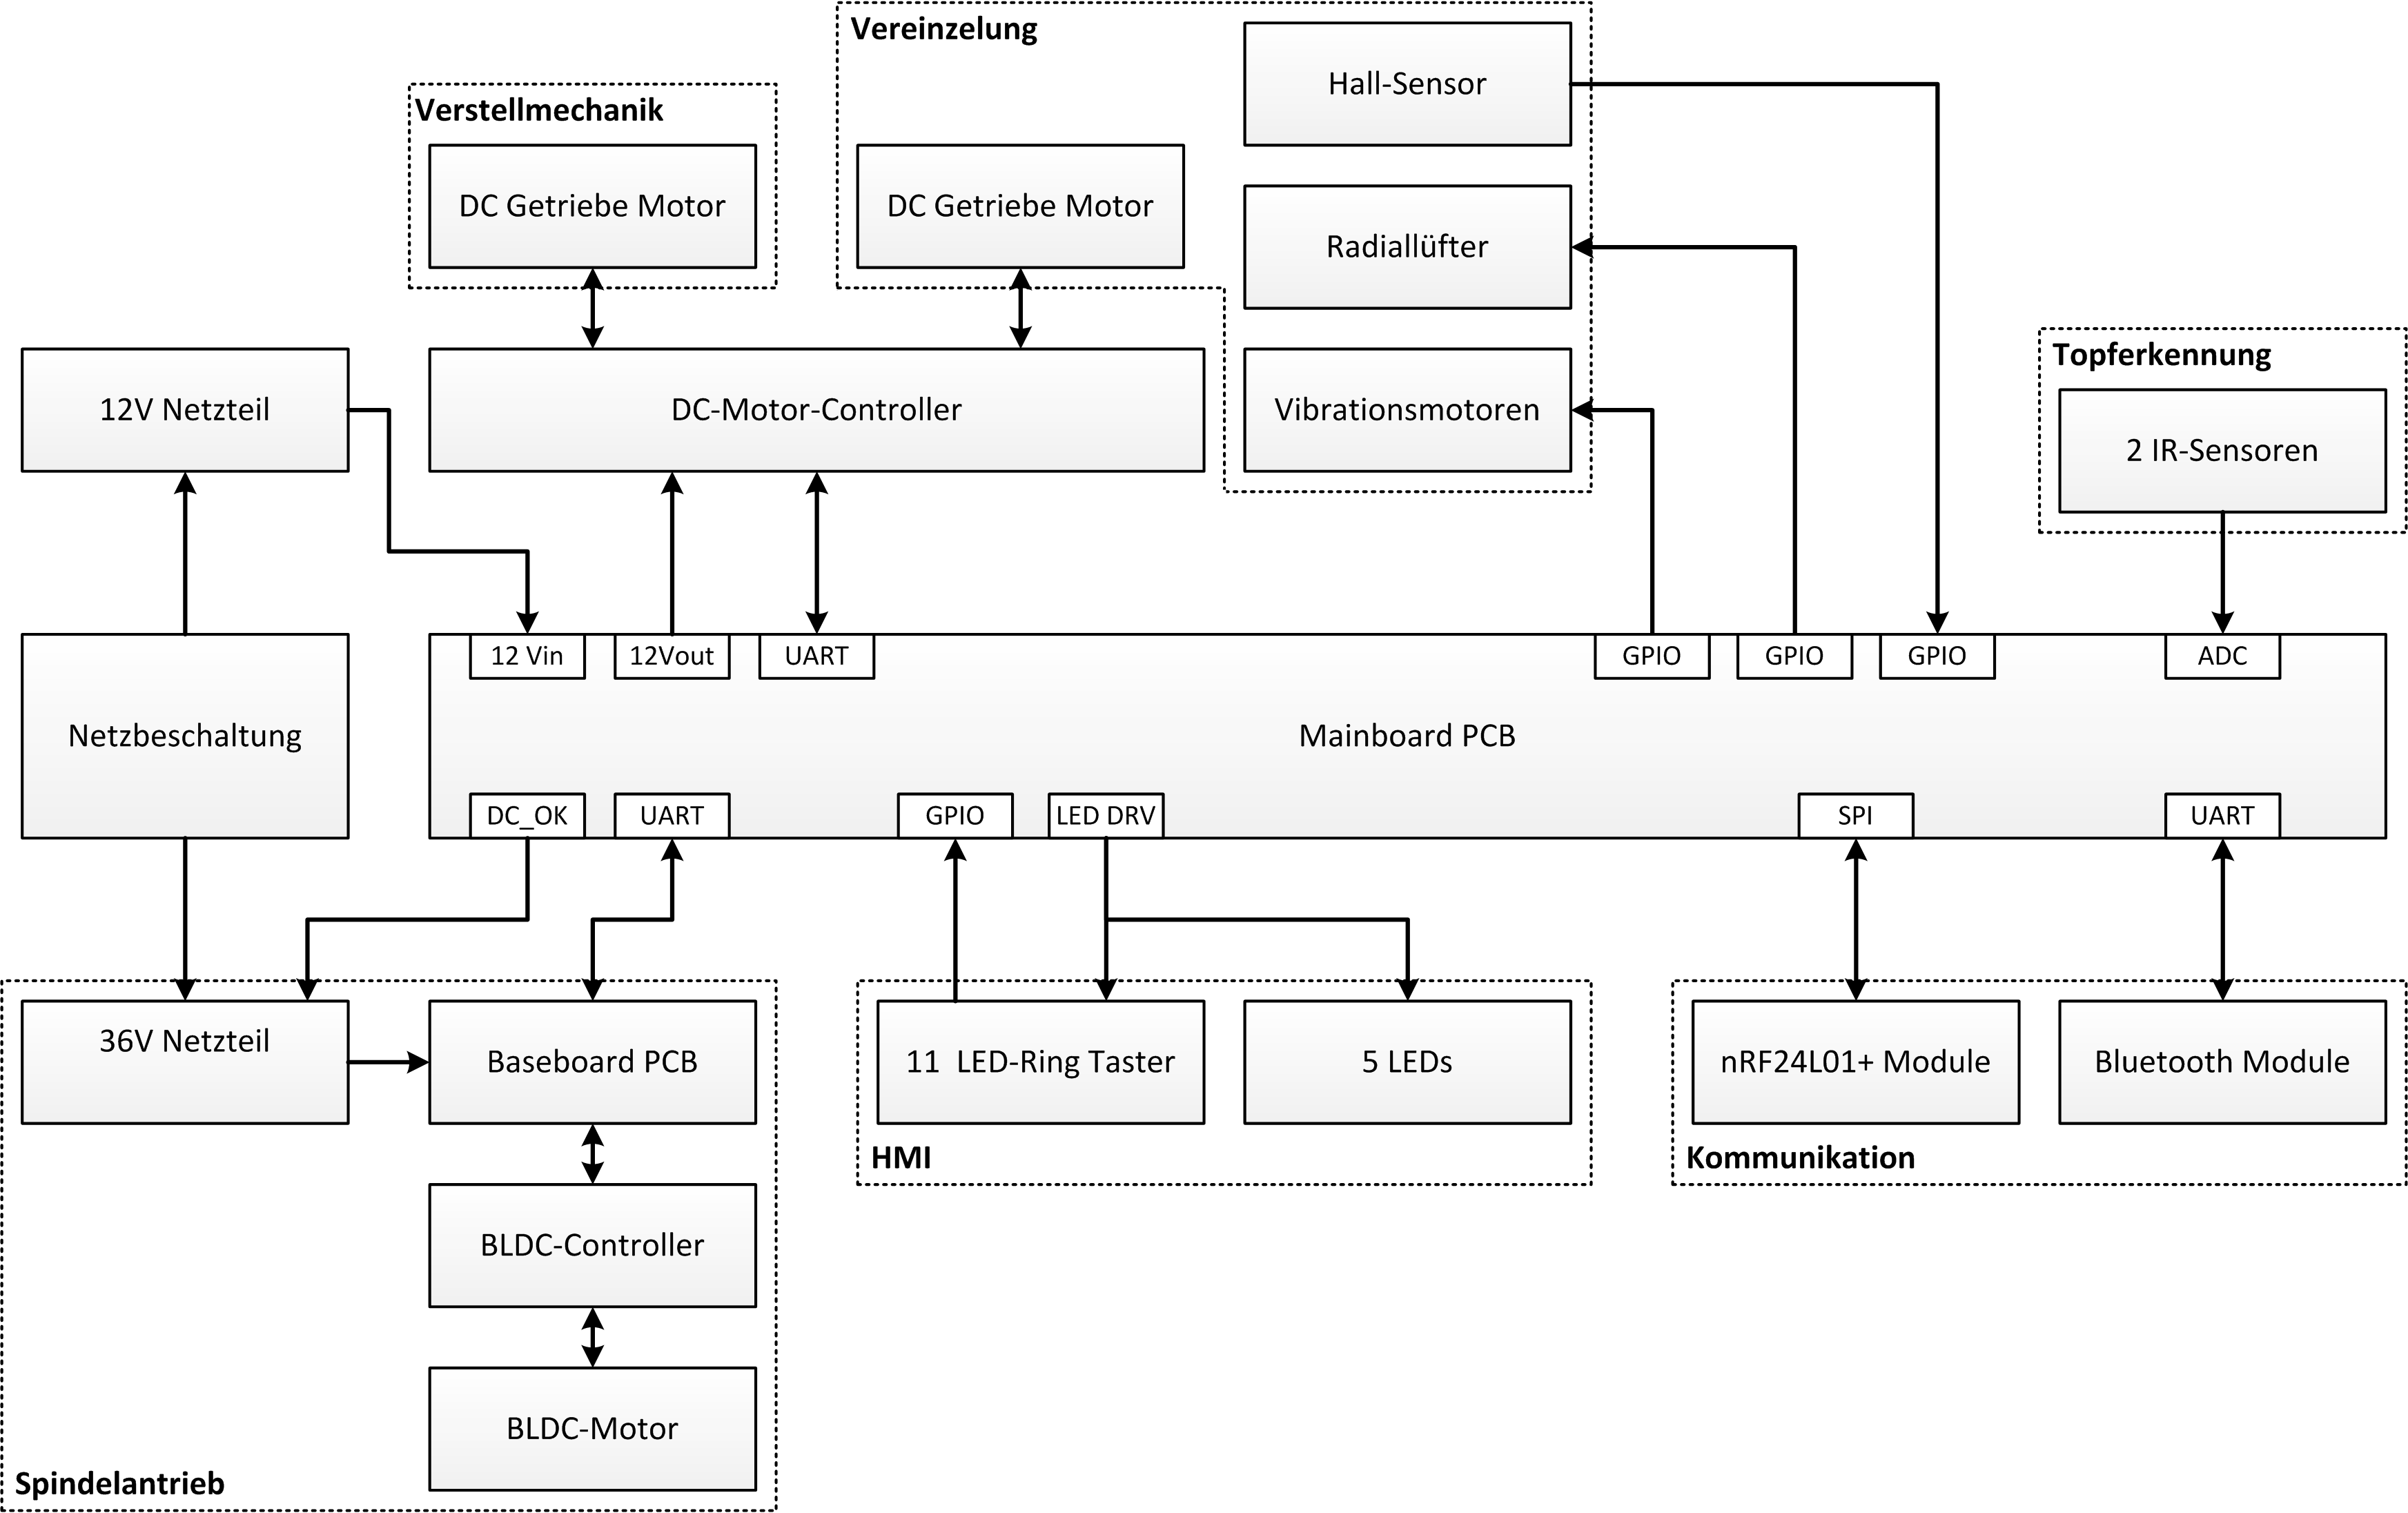
\includegraphics[width=1\textwidth]{Illustrationen/5-Konzept/Blockschaltbild_Komponenten.png}
	\caption{Blockschaltbild der Elektronik Komponenten}
	\label{fig:Blockschaltbild_Komponenten}
\end{figure}

Im folgenden Abschnitt wird das Blockschaltbild ausführlich erklärt:
\begin{itemize}
	\item \textbf{Netzbeschaltung:} Gemäss Pflichtenheft, soll der Planting Robot über 230V Netzspannung betrieben werden können. Diese Anforderung setzt eine adäquate Schutzschaltung voraus. So wurde ein Leitungsschutzschalter, sowie eine Relais Selbsthalteschaltung zum Ein und Ausschalten der Anlage über zwei Taster mit Betriebsanzeige vorgesehen. Des weiteren wurden sämtliche Gehäuseteile aus Metall, innerhalb des Schaltschrankes, mit dem Schutzleiter elektrisch verbunden.

	\item \textbf{36V Netzteil:} Um die hohe Leistungsanforderung an den Spindelantrieb bei moderatem Stromfluss erfüllen zu können, wird dessen Motor mit einem 36V Netzteil gespeist. Das FRDM-Board kann über das enable Signal des Netzteils die 36V Ausgangsspannung ein- und ausschalten.
	
	\item \textbf{BLDC-Controller:} Der BLDC-Controller wird über einen UART Port des FRDM-Boards angesteuert. Mit Hilfe der Encoder Auswertung des BLDC-Controllers kann der BLDC-Motor als Servomotor mit Positionsregelung betrieben werden. Damit kann ein Maximum an Präzision und Geschwindigkeit bei der Ansteuerung des Spindelantriebs garantiert werden.
	
	\item \textbf{Baseboard PCB:} Als Schnittstelle zwischen Mainboard PCB und BLDC-Controller dient das Baseboard PCB. Es vereinfacht die Verkabelung mit dem BLDC-Controller Board und verfügt über Drehpotentiometer zur schnellen Inbetriebnahme des BLDC-Motors.
	
	\item \textbf{Spindelantrieb:} Für eine maximale Lebensdauer bei häufigen Lastwechseln und ein hohes Anzugdrehmoment wird ein BLDC-Motor mit Hall Sensoren verwendet.
			
	\item \textbf{12V Netzteil:} Um einen sicheren Betrieb der Elektronik während hohen Leistungsspitzen des Spindelantriebs zu garantieren, wird diese über ein separates Netzteil versorgt. Des weiteren werden auch die kleineren DC Getriebemotoren über dieses Netzteil gespeist. Das 12V Netzteil wird über das Zuschalten der Netzspannung gesteuert und kann nicht über den Mikrocontroller geschaltet werden.
\end{itemize}
\subsection{Evaluation der Komponenten}
\subsection{Software}
\label{kap:Software}

\input{Kapitel/6_Umsetzung/6.0_Überblick}
\newpage
\section{Umsetzung}
\subsection{Mainboard PCB}

BLALBABLAL
\subsection{Software} \label{sec:Software}
\textit{(pro)} Die Software des Planting Robots ist in der Programmiersprache C geschrieben und läuft auf dem ARM Cortex M0+ Mikrocontroller von NXP welcher auf dem FRDM-Board KL25Z bestückt ist. Für low Level Driver werden diverse Processor Expert Komponenten verwendet. Als Betriebssystem dient das Real Time OS FreeRTOS. Vorteile von FreeRTOS gegenüber anderen C Betriebssystemen sind:

\begin{itemize}
	\item Seine geringen Ressourcenanforderungen an RAM, ROM und CPU Leistung. 
	\item FreeRTOS ist weit verbreitet und wird an der HSLU in diversen Softwareprojekten verwendet.
	\item Es ist absolut kostenfrei, auch für kommerzielle Anwendungen.
	\item FreeRTOS ist einfach in der Anwendung, eignet sich jedoch auch für grössere Projekte.
\end{itemize}

In den folgenden Unterkapiteln werden die wichtigsten Softwarekomponenten des Planting Robots beschrieben und erklärt. Die Titel der Unterkapitel korrespondieren dabei mit den Namen der .c Files des Codes im Anhang.

\subsubsection{FSM} \label{sec:FSM}
Der Planting Robot wird durch einen endlichen Zustandsautomaten FSM gesteuert. Die Zustände oder States die FSM sind in Abb. \ref{fig:FSM} illustriert. Ein State Wechsel wird entweder durch eine User Eingabe übe das HMI, eine Topferkennung durch den IR-Sensor oder durch fertigstellen eines States ausgeführt. Im folgenden Abschnitt werden die verschiedenen States sowie State-Wechsel erklärt:

\begin{figure}[H]
	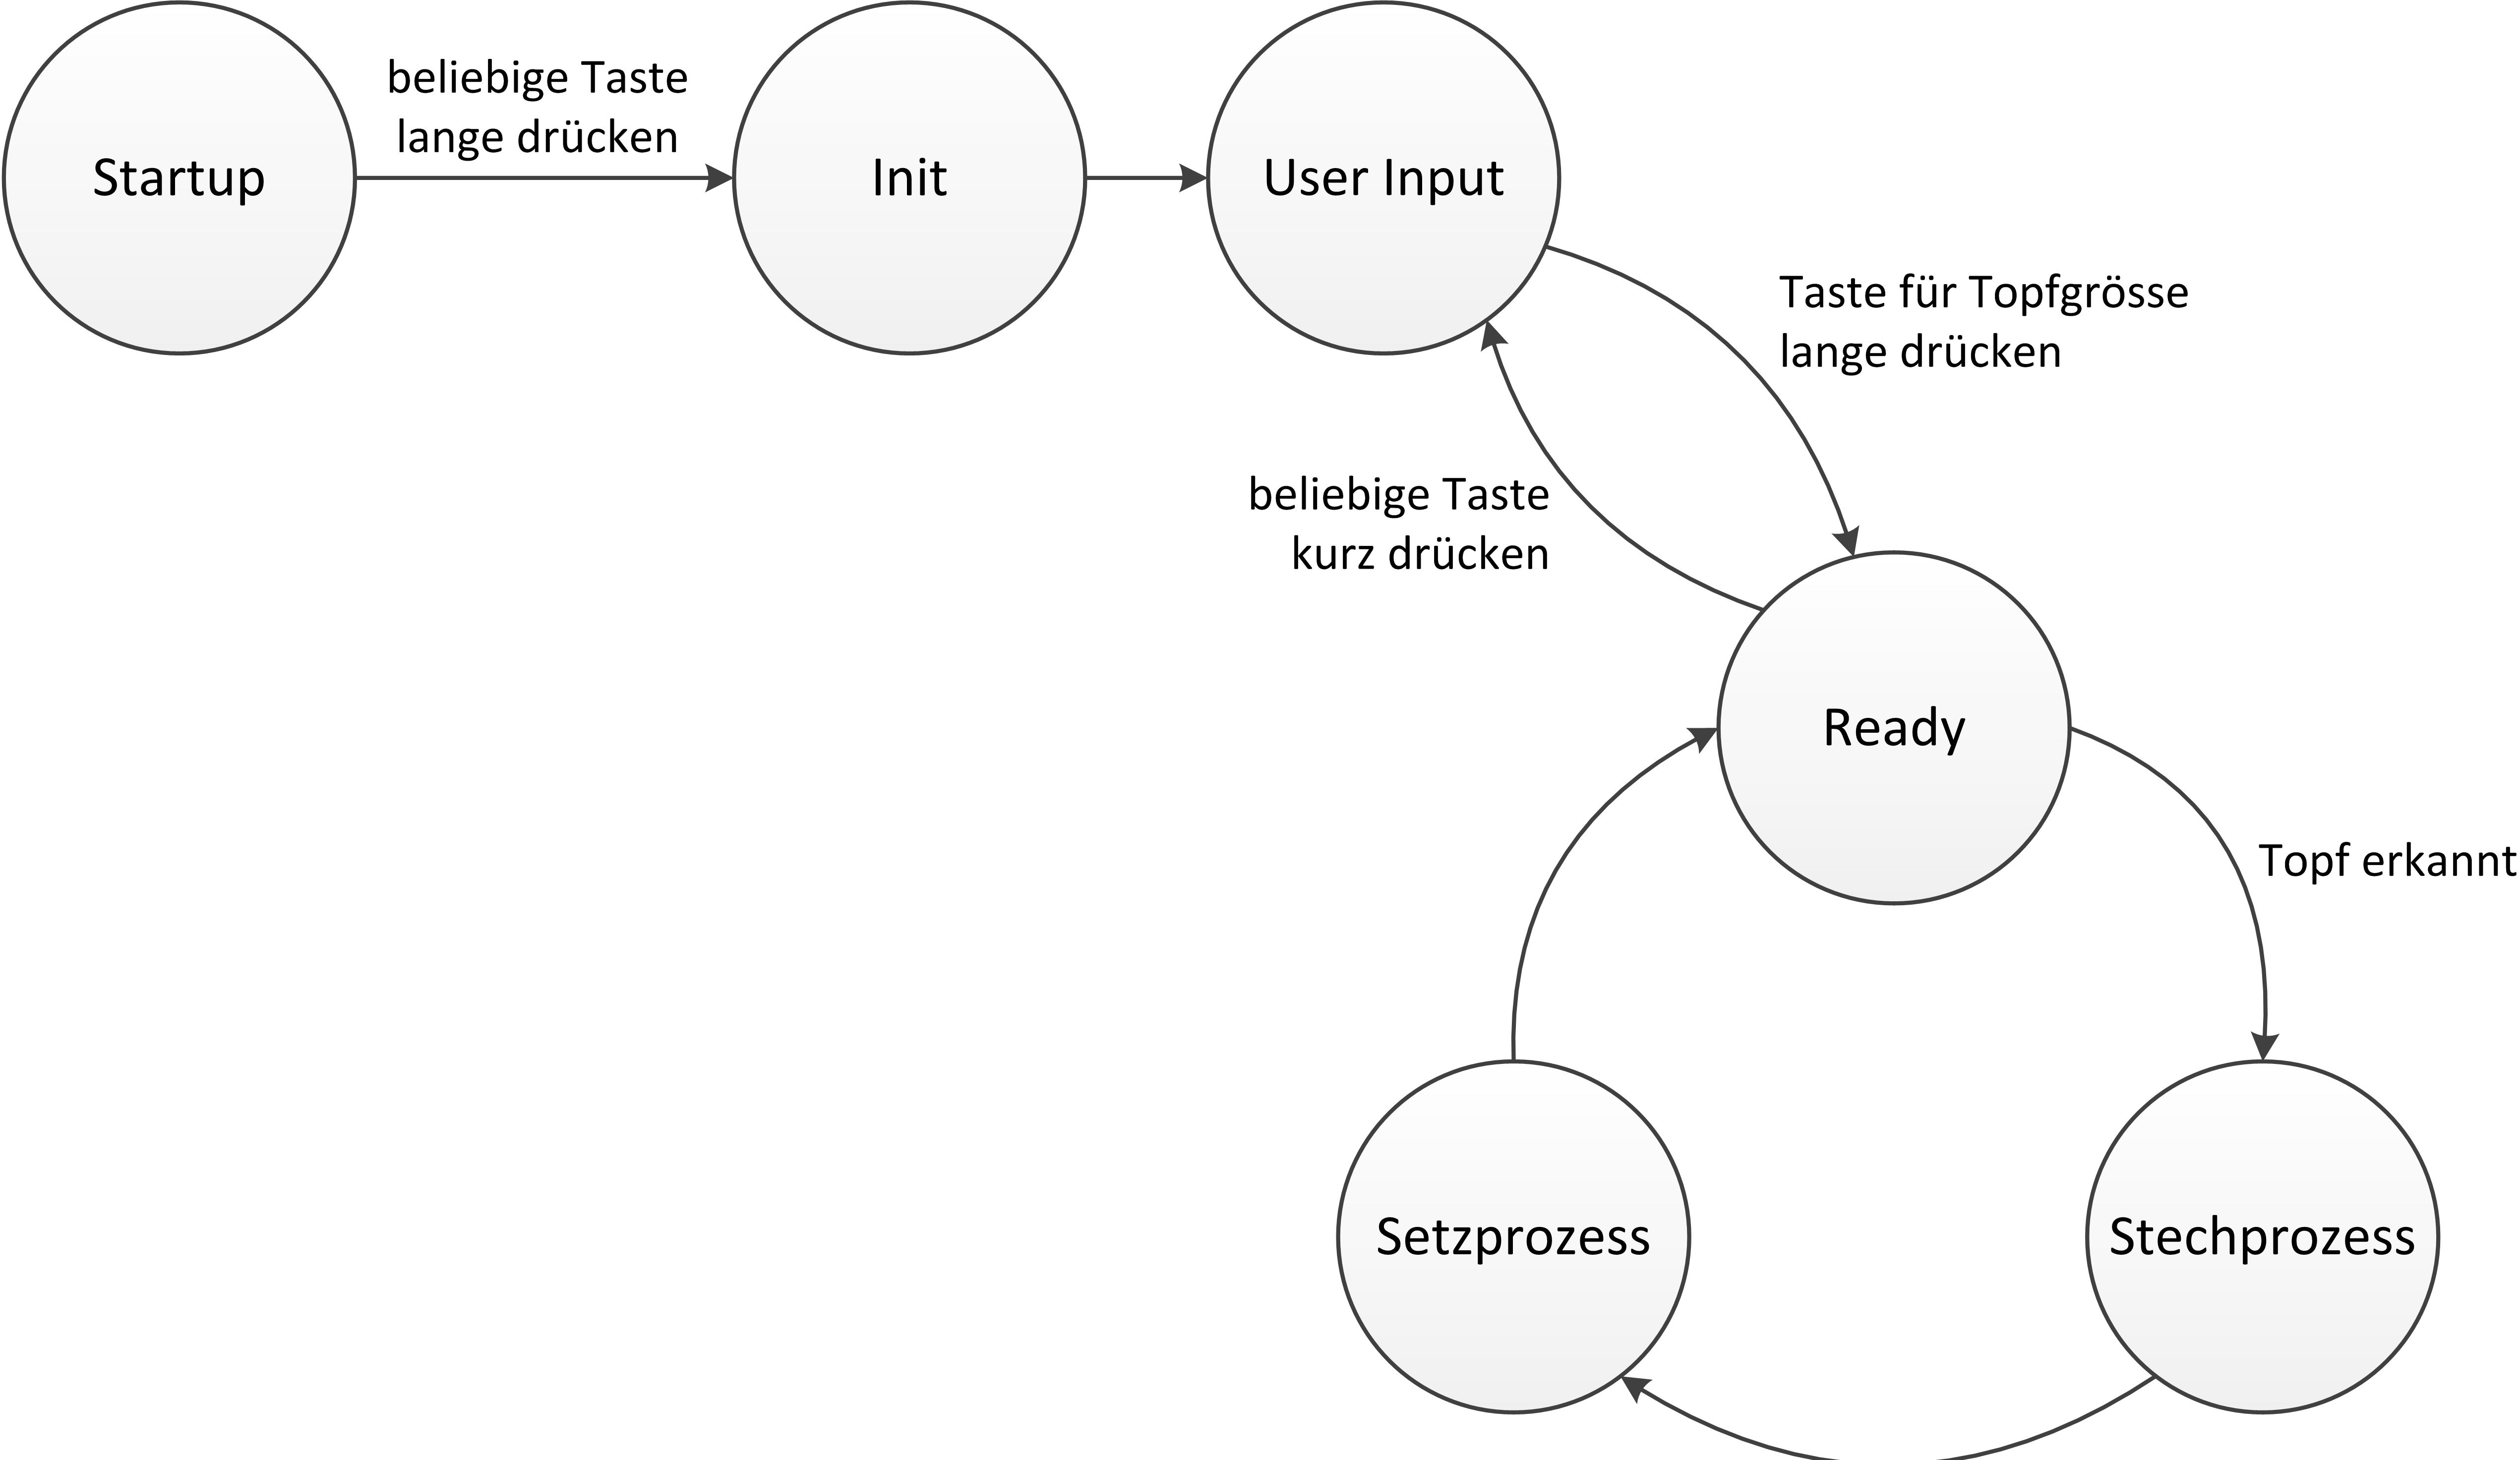
\includegraphics[width=0.9\textwidth]{Illustrationen/6-Umsetzung/FSM_B&W_breit.png}
	\caption{Software, FSM}
	\label{fig:FSM}
\end{figure}

\textbf{Startup:} Wenn die Speisung zum uC eingeschaltet wird, begibt sich die Software in den sicheren Zustand $"$Startup$"$. In diesem State sind sämtliche Aktoren stromlos. Alle LEDs des HMIs pulsieren synchron. Wird ein beliebiger Taster des HMIs länger als eine halbe Sekunde gedrückt wechselt die Software in den $"$Init$"$ State.\\
\newline
\textbf{Init:} In diesem State werden die Motoren für die Vereinzelung, die Verstellmechanik und die Setzeinheit initialisiert. Da die Motoren über Drehencoder und nicht über absolute Positionsencoder verfügen, müssen diese zuerst in ihre Ausgangsposition gebracht werden. Der Initialisierungsprozess zu den jeweiligen Motoren wird in den Kapiteln \ref{sec:Vereinzelung}, \ref{sec:Setzeinheit} und \ref{verstellmechanik} erklärt. Während der Initialisierung blinken die HMI LEDs des jeweiligen Prozesses. Nach Abschluss der Initialisierung wechselt die State Machine in den $"$User Input$"$ State.\\
\newline
\textbf{User Input:} Dieser State dient zur Konfiguration des Planting Robots. Der Operator kann hier die Topfgrösse des aktuellen Batches und die Setztiefe der Nemacaps über das HMI einstellen. Ausserdem kann der Planting Robot in diesem State manuell über die Tasten $"$manuelle Steuerung$"$ bedient werden. Mehr zur manuellen Steuerung ist im Kapitel \ref{sec:HMI} nachzulesen. Um die Konfiguration zu speichern und den Planting Robot in Betrieb zu setzen muss der Taster für die gewünschte Topfgrösse lange gedrückt werden.\\
\newline
\textbf{Ready:} Der Planting Robot befindet sich im regulären Betriebsmodus. Sobald ein Topf erkannt wird, verrichtet der Planting Robot seine Arbeit indem er den Stechprozess und anschliessend den Setzprozess ausführt. Um den Planting Robot zu stoppen, kann ein beliebiger Taster gedrückt werden. Der Planting Robot wechselt dann zurück in den $"$User Input$"$ State.\\
\newline
\textbf{Stechprozess:} Dieser Prozess wird durchlaufen sobald ein Topf erkannt wurde. Dabei wird mit dem Spindelantrieb eine Hubbewegung ausgeführt bei welcher der Stechdorn in die Erde gedrückt und wieder angehoben wird.\\
\newline
\textbf{Setzprozess:} Sobald der Stechprozess beendet ist wird der Setzprozess ausgeführt. Dabei wird die Vereinzlung angetrieben, sodass NemaCaps vom Schüttgutlager in die Topferde befördert wird. Nach beenden des Setzprozesses geht die FSM wieder in den $"$Ready$"$ State.

\subsubsection{HMI Driver}
Im HMI\_Driver.c File wird der HMI\_Task erzeugt. Alle 10ms führt dieser den Debounce Prozess aus. Dabei wird die Funktion FunktionKEYDBNC\_Process() aufgerufen, welche den Status aller Taster des HMIs ausliest und über eine State Machine entprellt. Der Debounce Prozess generiert dann ein Event für jeden Tastendruck, langen Tastendruck und loslassen eines Tasters. Events werden vom Event.c File in einem Event Array abgespeichert. Es wird somit ein Polling der HMI Taster mit einer Frequenz von 100Hz durchgeführt. Diese Programmsequenz ist in Abb. \ref{fig:Taster_Polling} oben grafisch dargestellt.


\begin{figure}[H]
	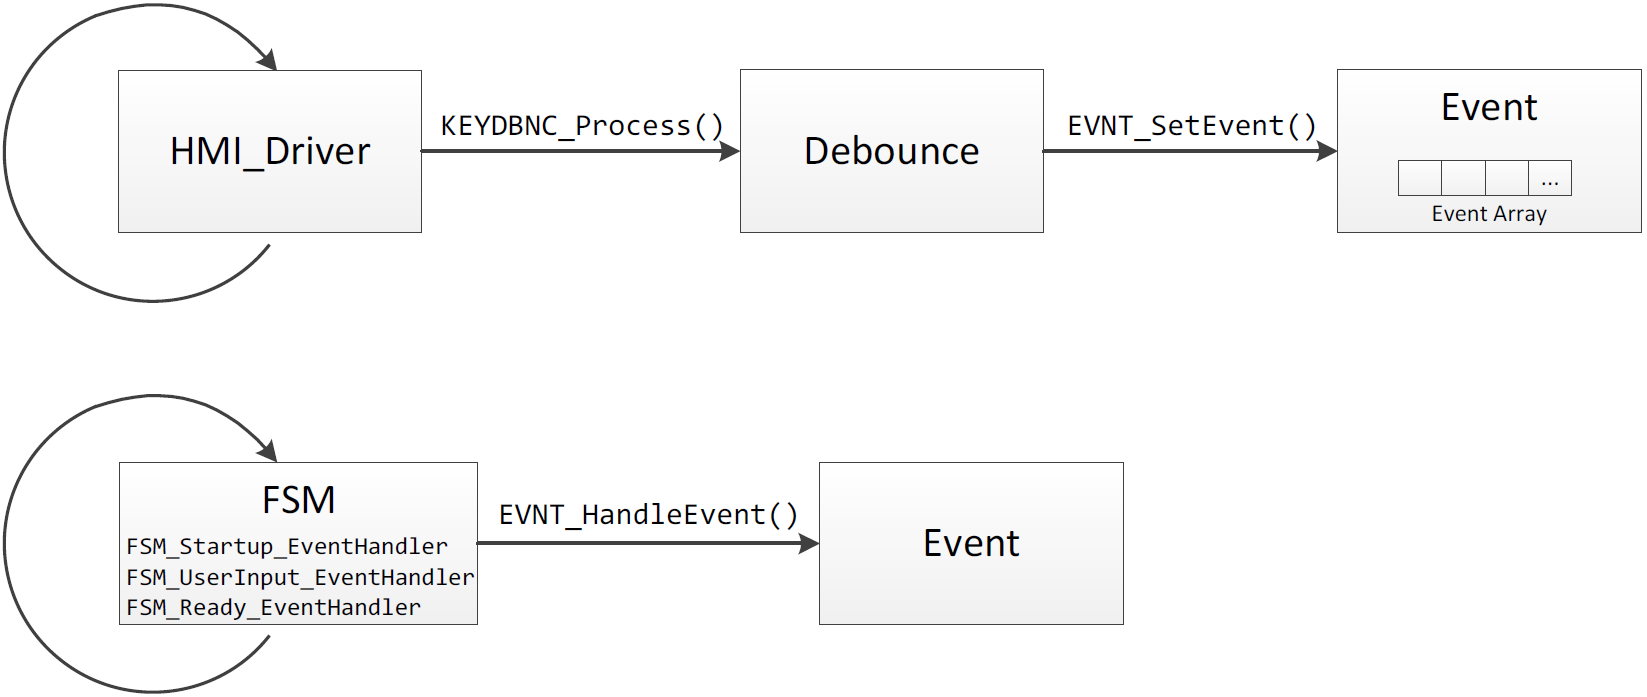
\includegraphics[width=0.9\textwidth]{Illustrationen/6-Umsetzung/Taster_Polling.png}
	\caption{Software, Taster Polling / Auswertung}
	\label{fig:Taster_Polling}
\end{figure}

Der untere Teil der Grafik in Abb. \ref{fig:Taster_Polling} beschreibt die Auswertung eines Tastendrucks. Dazu werden die vom Debounce Prozess erzeugte Events in einem der drei Eventhandler (FSM\_Startup\_EventHandler, FSM\_UserInput\_EventHandler oder FSM\_Ready\_EventHandler) des FSM.c Files ausgewertet. Eine solche Taster Event Auswertung ist am Beispiel des FSM\_Startup\_EventHandler im folgenden Code dargestellt:

\begin{lstlisting}
void FSM_Startup_EventHandler(EVNT_Handle event) {
	switch(event) {
		case EVNT_BTN_9cm_LPRESSED:				// Any Button Long Press
		case EVNT_BTN_11cm_LPRESSED:
		case EVNT_BTN_12cm_LPRESSED:
		case EVNT_BTN_13cm_LPRESSED:
		case EVNT_BTN_14cm_LPRESSED:
		case EVNT_BTN_AUTO_LPRESSED:
		case EVNT_BTN_Setzeinheit_runter_LPRESSED:
		case EVNT_BTN_Setzeinheit_hoch_LPRESSED:
		case EVNT_BTN_Vereinzelung_LPRESSED:
		case EVNT_BTN_hoeher_LPRESSED:
		case EVNT_BTN_tiefer_LPRESSED:
			LED_Driver_pulseAll(FALSE);
			LED_Driver_clear_all();
			fsmData.fsmState = Init;
			break;
		default:
			break;
	} /* switch */
}
\end{lstlisting}

Der Code beschreibt das Verhalten des Planting Robots auf einen Tastendruck während des Startup States wie in Kapitel \ref{sec:FSM} beschrieben. \\
\newline
Die .c Files Debounce, Event, KeyDebounce und Trigger beruhen Grundlegend auf den Gleichnamigen Files aus dem Modulunterricht INTRO, betreut durch Erich Styger. Der Code wurde jedoch für die Verwendung mit dem Planting Robot angepasst und erweitert.

\subsubsection{LED Driver}
Wie in Kapitel \ref{sec:Mainboard_HMI_Interface} erklärt, wird für die Ansteuerung der HMI LEDs der LED Treiber Baustein LP3943, mit I$^{2}$C Schnittstelle verwendet. Die I$^{2}$C Schnittstellenparameter wurden gemäss Tabelle \ref{tab:I2C_Parameter} in Processor Expert konfiguriert:

\begin{table}[H]
	\centering
	\caption{Software, I$^{2}$C Parameter LED Treiber}
	\begin{tabular}{|l|c|r|}
		\hline
		\textbf{Parameter} & \textbf{Wert} & \textbf{Einheit} \\
		\hline
		SCL frequency & 109.227 & kHz \\
		\hline
		SDA Hold & 0.811 & us \\
		\hline
		SCL start Hold & 4.482 & us \\
		\hline
		SCL stop Hold & 4.625 & us \\
		\hline
		Adress mode & 7     & bit \\
		\hline
	\end{tabular}%
	\label{tab:I2C_Parameter}%
\end{table}%

In Tabelle \ref{tab:LP3943_Register} sind sämtliche Funktions Register des LP3943 aufgelistet. Die LEDs des HMI können durch schreiben der Register LS0... LS3 konfiguriert werden. Dabei kann jeder LED Port einen der folgenden vier Konfigurationen annehmen: LED aus, LED ein, LED dimmen mit Dimmrate DIM0, LED dimmen mit Dimmrate DIM1. Die Dimmraten DIM0 und DIM1 sind durch Timer Bausteine definiert. Demnach kann für jeden der beiden Timer über die Register Prescaler und PWM eine Frequenz und ein Tastgrad konfiguriert werden. Da über das Prescaler Register eine Periodenzeit von 6.25ms... 1.6s eingestellt werden kann, können die LEDs gut sichtbar zum blinken gebracht werden.

\begin{table}[H]
	\centering
	\caption{LP3943 Register Tabelle \protect\cite{LP3943}}
	\begin{tabular}{|l|l|l|l|}
		\hline
		\textbf{Adress (Hex)} & \textbf{Register Name} & \textbf{Read/Write} & \textbf{Register Function} \\
		\hline
		0x00  & Input 1 & Read only & LED0–7 Input Register \\
		\hline
		0x01  & Input 2 & Read only & LED8–15 Input Register \\
		\hline
		0x02  & PSC0  & R/W   & Frequency Prescaler 0 \\
		\hline
		0x03  & PWM0  & R/W   & PWM Register 0 \\
		\hline
		0x04  & PSC1  & R/W   & Frequency Prescaler 1 \\
		\hline
		0x05  & PWM1  & R/W   & PWM Register 1 \\
		\hline
		0x06  & LS0   & R/W   & LED0–3 Selector \\
		\hline
		0x07  & LS1   & R/W   & LED4–7 Selector \\
		\hline
		0x08  & LS2   & R/W   & LED8–11 Selector \\
		\hline
		0x09  & LS3   & R/W   & LED12–15 Selector \\
		\hline
	\end{tabular}%
	\label{tab:LP3943_Register}%
\end{table}%

Durch Verwendung der Register Input 1 sowie Input 2 können die Pins des LP3943 auch als Digital Inputs verwendet werden. In diesem Projekt wird der LP3943 allerdings nur zum treiben von LEDs verwendet.

\subsubsection{ION Motion Driver}

\subsubsection{IR Sensor Driver}

\subsubsection{Trinamic Motion Driver}
\subsection{Vereinzelung} \label{sec:Vereinzelung}
\textit{(ygu)} Die Umsetzung der Vereinzelung orientiert sich stark am realisierten Funktionsnachweis. Der grundlegende Aufbau wurde beibehalten. Hinzu kommen einige Erweiterungen, um die Zuverlässigkeit zu steigern sowie Verbesserungen in der Benutzerfreundlichkeit zu erreichen.
\newline

\textbf{Aufbau und Funktion}
\newline
Die Vereinzelung besteht aus einer Trommel (Punkt. 1 in Abbildung \ref{fig:details_vereinzelung}), worin die NemaCaps eingefüllt werden. Durch die Rotation der Lochmaske (3), welche durch einen Getriebemotor (7) umgesetzt wird, fallen die NemaCaps in die vorgesehenen Löcher. Überschüssige NemaCaps werden durch mehrere Bürsten (6) abgestreift. Sobald die vereinzelten NemaCaps bei den Schlauchkupplungen (8) angekommen sind, sollen diese durch die Schläuche zur Einsetzlokalität fallen. Alle Komponenten werden auf einer Grundplatte (4) montiert, wobei diese in ihrer Neigung verstellbar gelagert ist.
	\begin{figure}[H]
	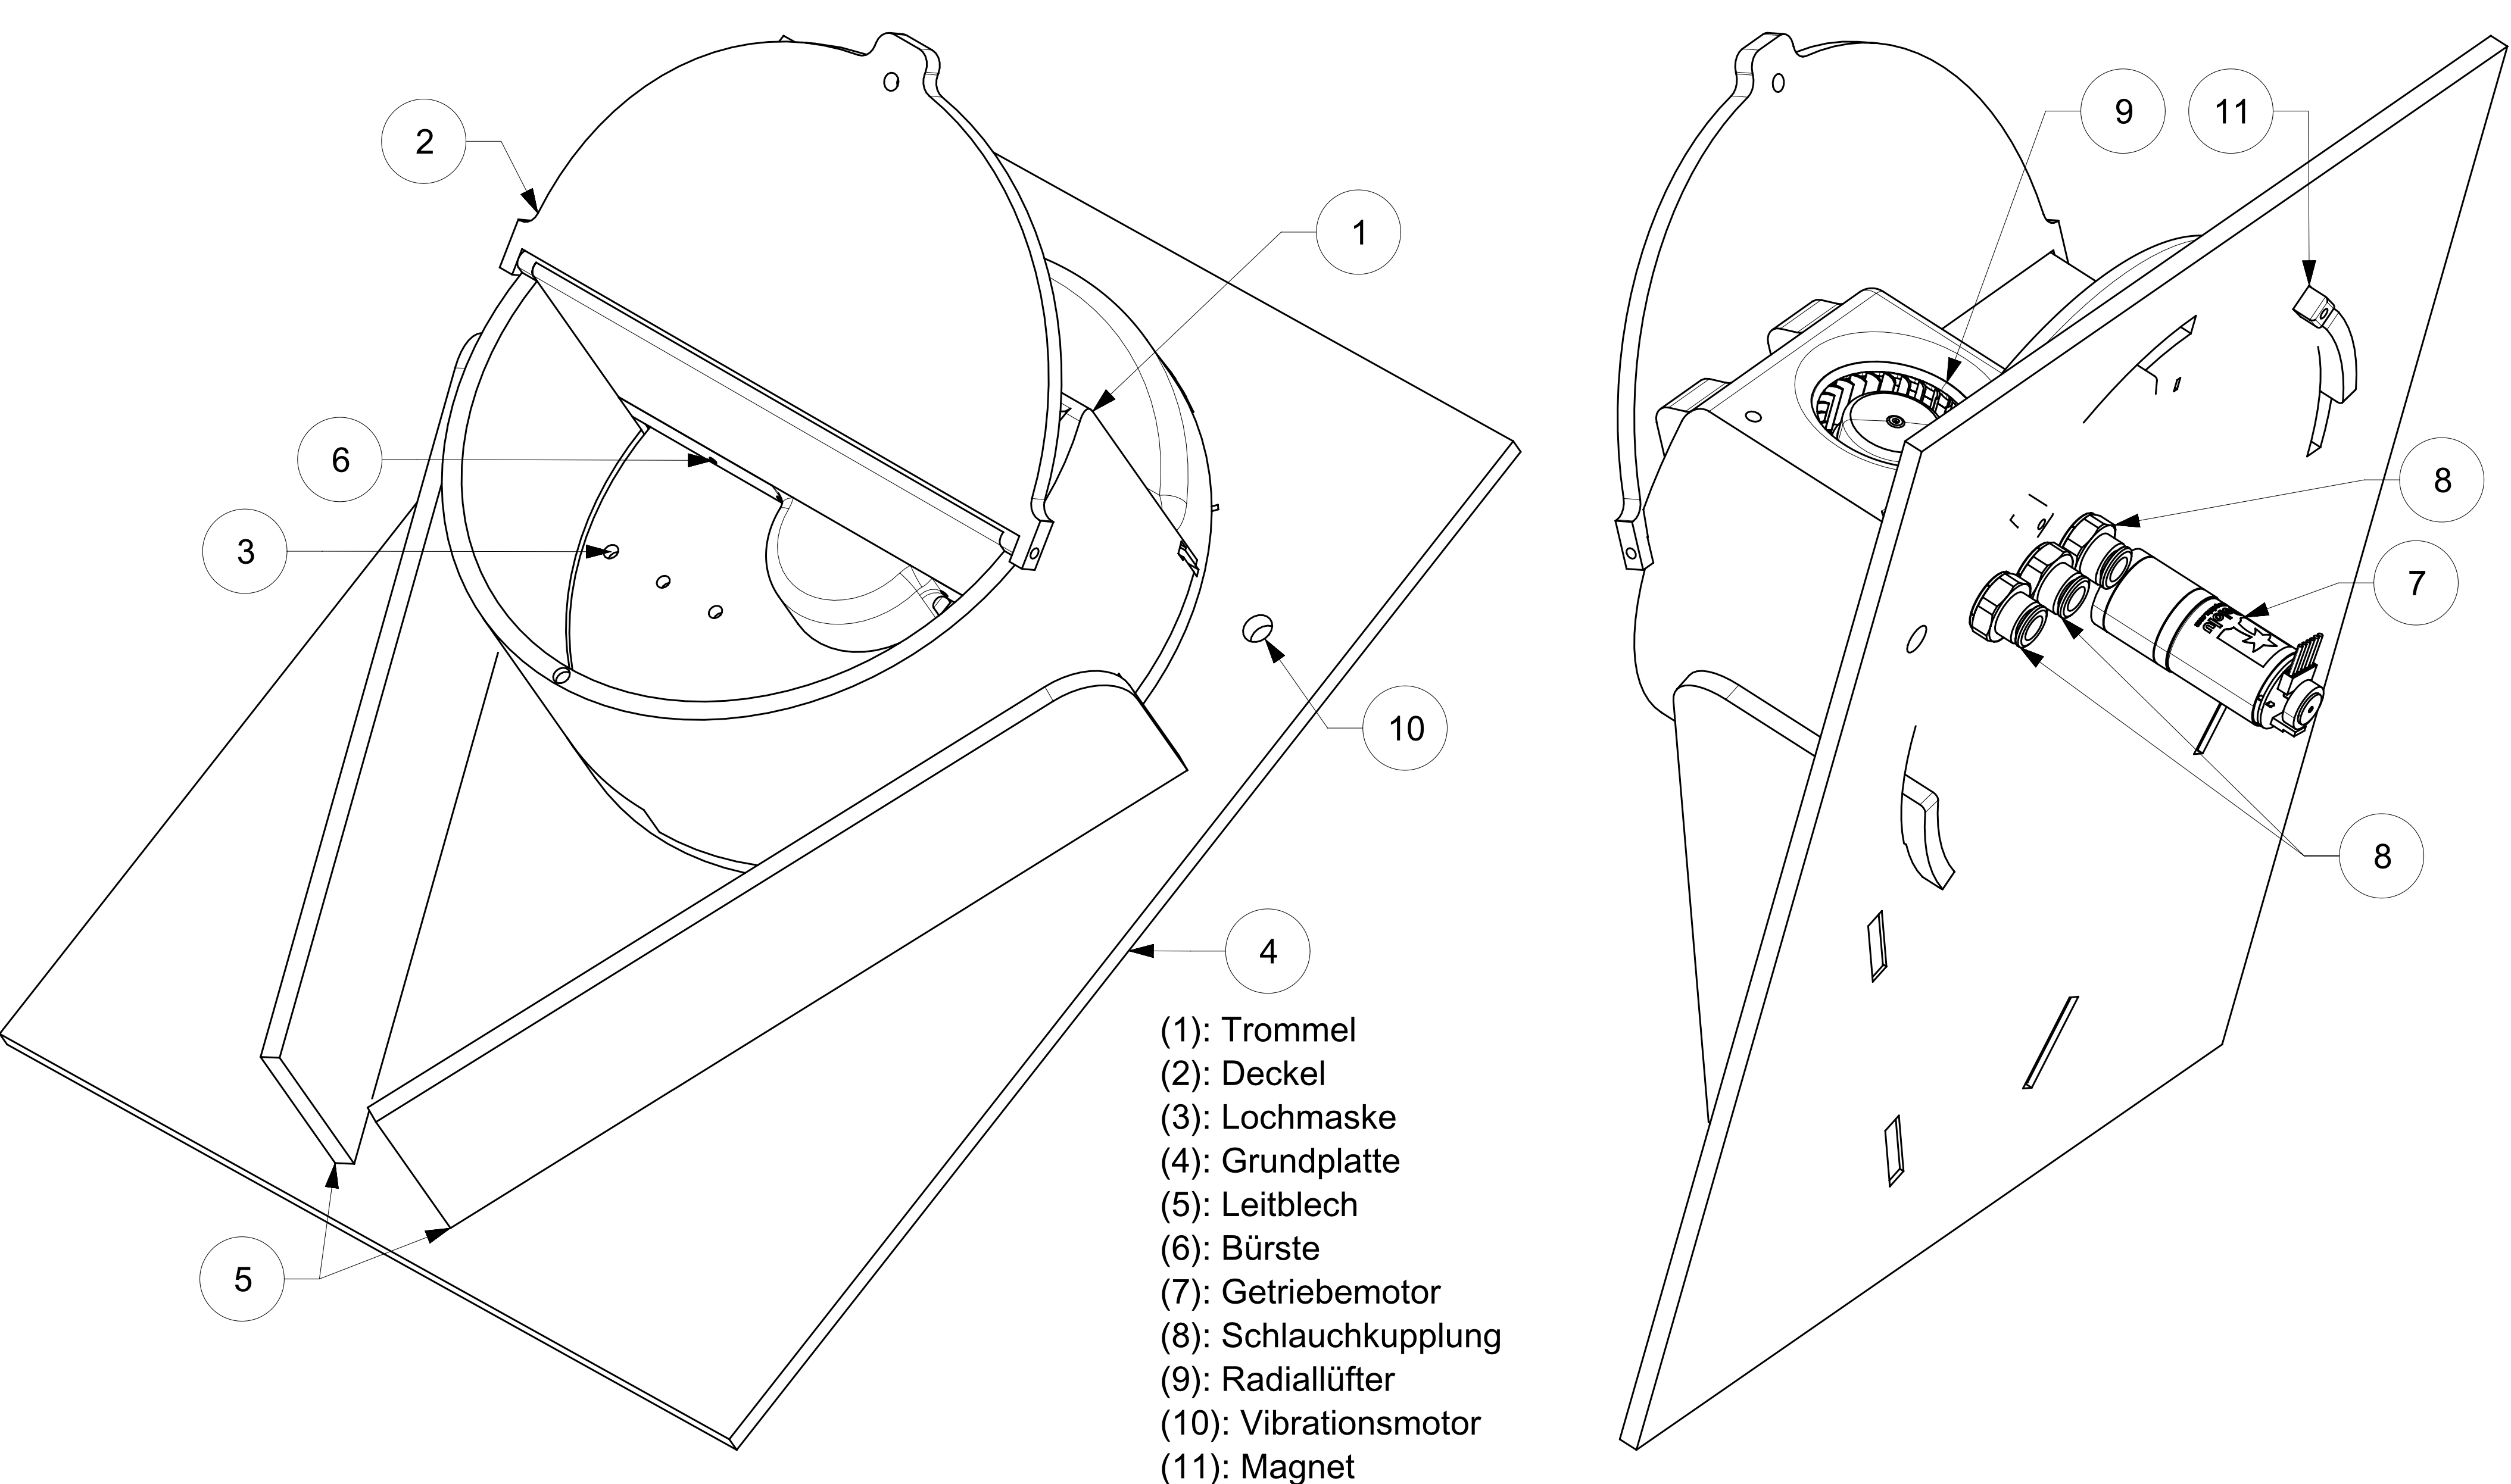
\includegraphics[scale=0.455]{Illustrationen/6-Umsetzung/details_vereinzelung.jpg}
	\caption{Detaillierte Übersicht der Vereinzelung}
	\label{fig:details_vereinzelung}
	\end{figure}
\newpage
\textbf{Abhilfemassnahmen}
\newline
Der Funktionsnachweis aus Kapitel \ref{funktionsnachweis} zeigte auf, dass Komplikationen auftretten können. In erschwerten Bedingungen, wie nassem Pulver, kann das NemaCap  durch die erhöhte Adhäsion an der Lochmaske hängen bleiben. So wurde im Funktionsnachweis die Bedingung formuliert, dass eine Umsetzung dieser Funktion nur mit konkreten Abhilfemassnahmen umgesetzt werden darf, um die Zuverlässigkeit der Vereinzelung zu steigern. Diese sind:
\begin{itemize}
	\item \textbf{Vibrationsmotor:} Der Funktionsnachweis zeigte, dass durch leichtes Klopfen an der Einheit, hängengebliebene NemaCaps erfolgreich gelöst werden. Somit wird in der Nähe der Schlauchkupplungen ein Vibrationsmotor (Punkt. 10 in Abbildung \ref{fig:details_vereinzelung}) angebracht, welche die Einheit in Schwingung bringen soll. Wichtig ist dabei, dass die Grundplatte in eine Richtung federnd gelagert wird, sodass diese tatsächlich in Schwingung geraten kann.
	
	\item \textbf{Radiallüfter:} Eine weitere Möglichkeit die NemaCaps zu lösen, bietet ein gezielter Luftstoss. Daher ist in der Trommel ein Radiallüfter (9) integriert, welcher einen Luftstrom auf die vereinzelten NemaCaps in der Lochmaske richtet. Bei Bedarf werden zusätzliche Löcher an den Schläuchen angebracht, um den Luftaustritt zu verbessern. 
	
	\item \textbf{Lochmaske:} Am Funktionsnachweis wurde ersichtlich, wie kritisch die Materialwahl sowie Fertigungsqualität der Lochmaske ist. Die formulierten Punkte zur Steigerung der Zuverlässigkeit sind in diesem Kapitel unter \textit{Lochmaske} \textbf{(anders markieren?)} erläutert.
\end{itemize}

\textbf{Handhabung}
\newline
Die Verwendung von frischen NemaCaps und somit frischem Pulver trägt zur verbesserten Zuverlässigkeit der Vereinzelung bei. Der benutzerfreundliche Wechsel von NemaCaps ist also ein wichtiges Anliegen und ist in der Konstruktion der Vereinzelung berücksichtigt. So ist die Trommel (Punkt 1 in Abb. \ref{fig:vereinzelung_entleeren}) mit einem dreifachen Bajonettverschluss (Detail C, 12) versehen. Die Trommel kann mit einer Drehung von 15° im Gegenuhrzeigersinn entriegelt werden (Detail A in Abb. \ref{fig:vereinzelung_entleeren}). Nun kann die Trommel entfernt werden (Detail B). Die verbleibenden NemaCaps (Detail X) rollen nun auf der Grundplatte hinunter. Gelenkt durch zwei Leitbleche (5) fallen diese in Richtung Detail Y, wo man diese in einem Behälter sammeln kann. Auch verfügt die Trommel über einen Deckel (2), welcher durch zwei angebrachte Magnete sicher verschlossen wird.
	\begin{figure}[H]
	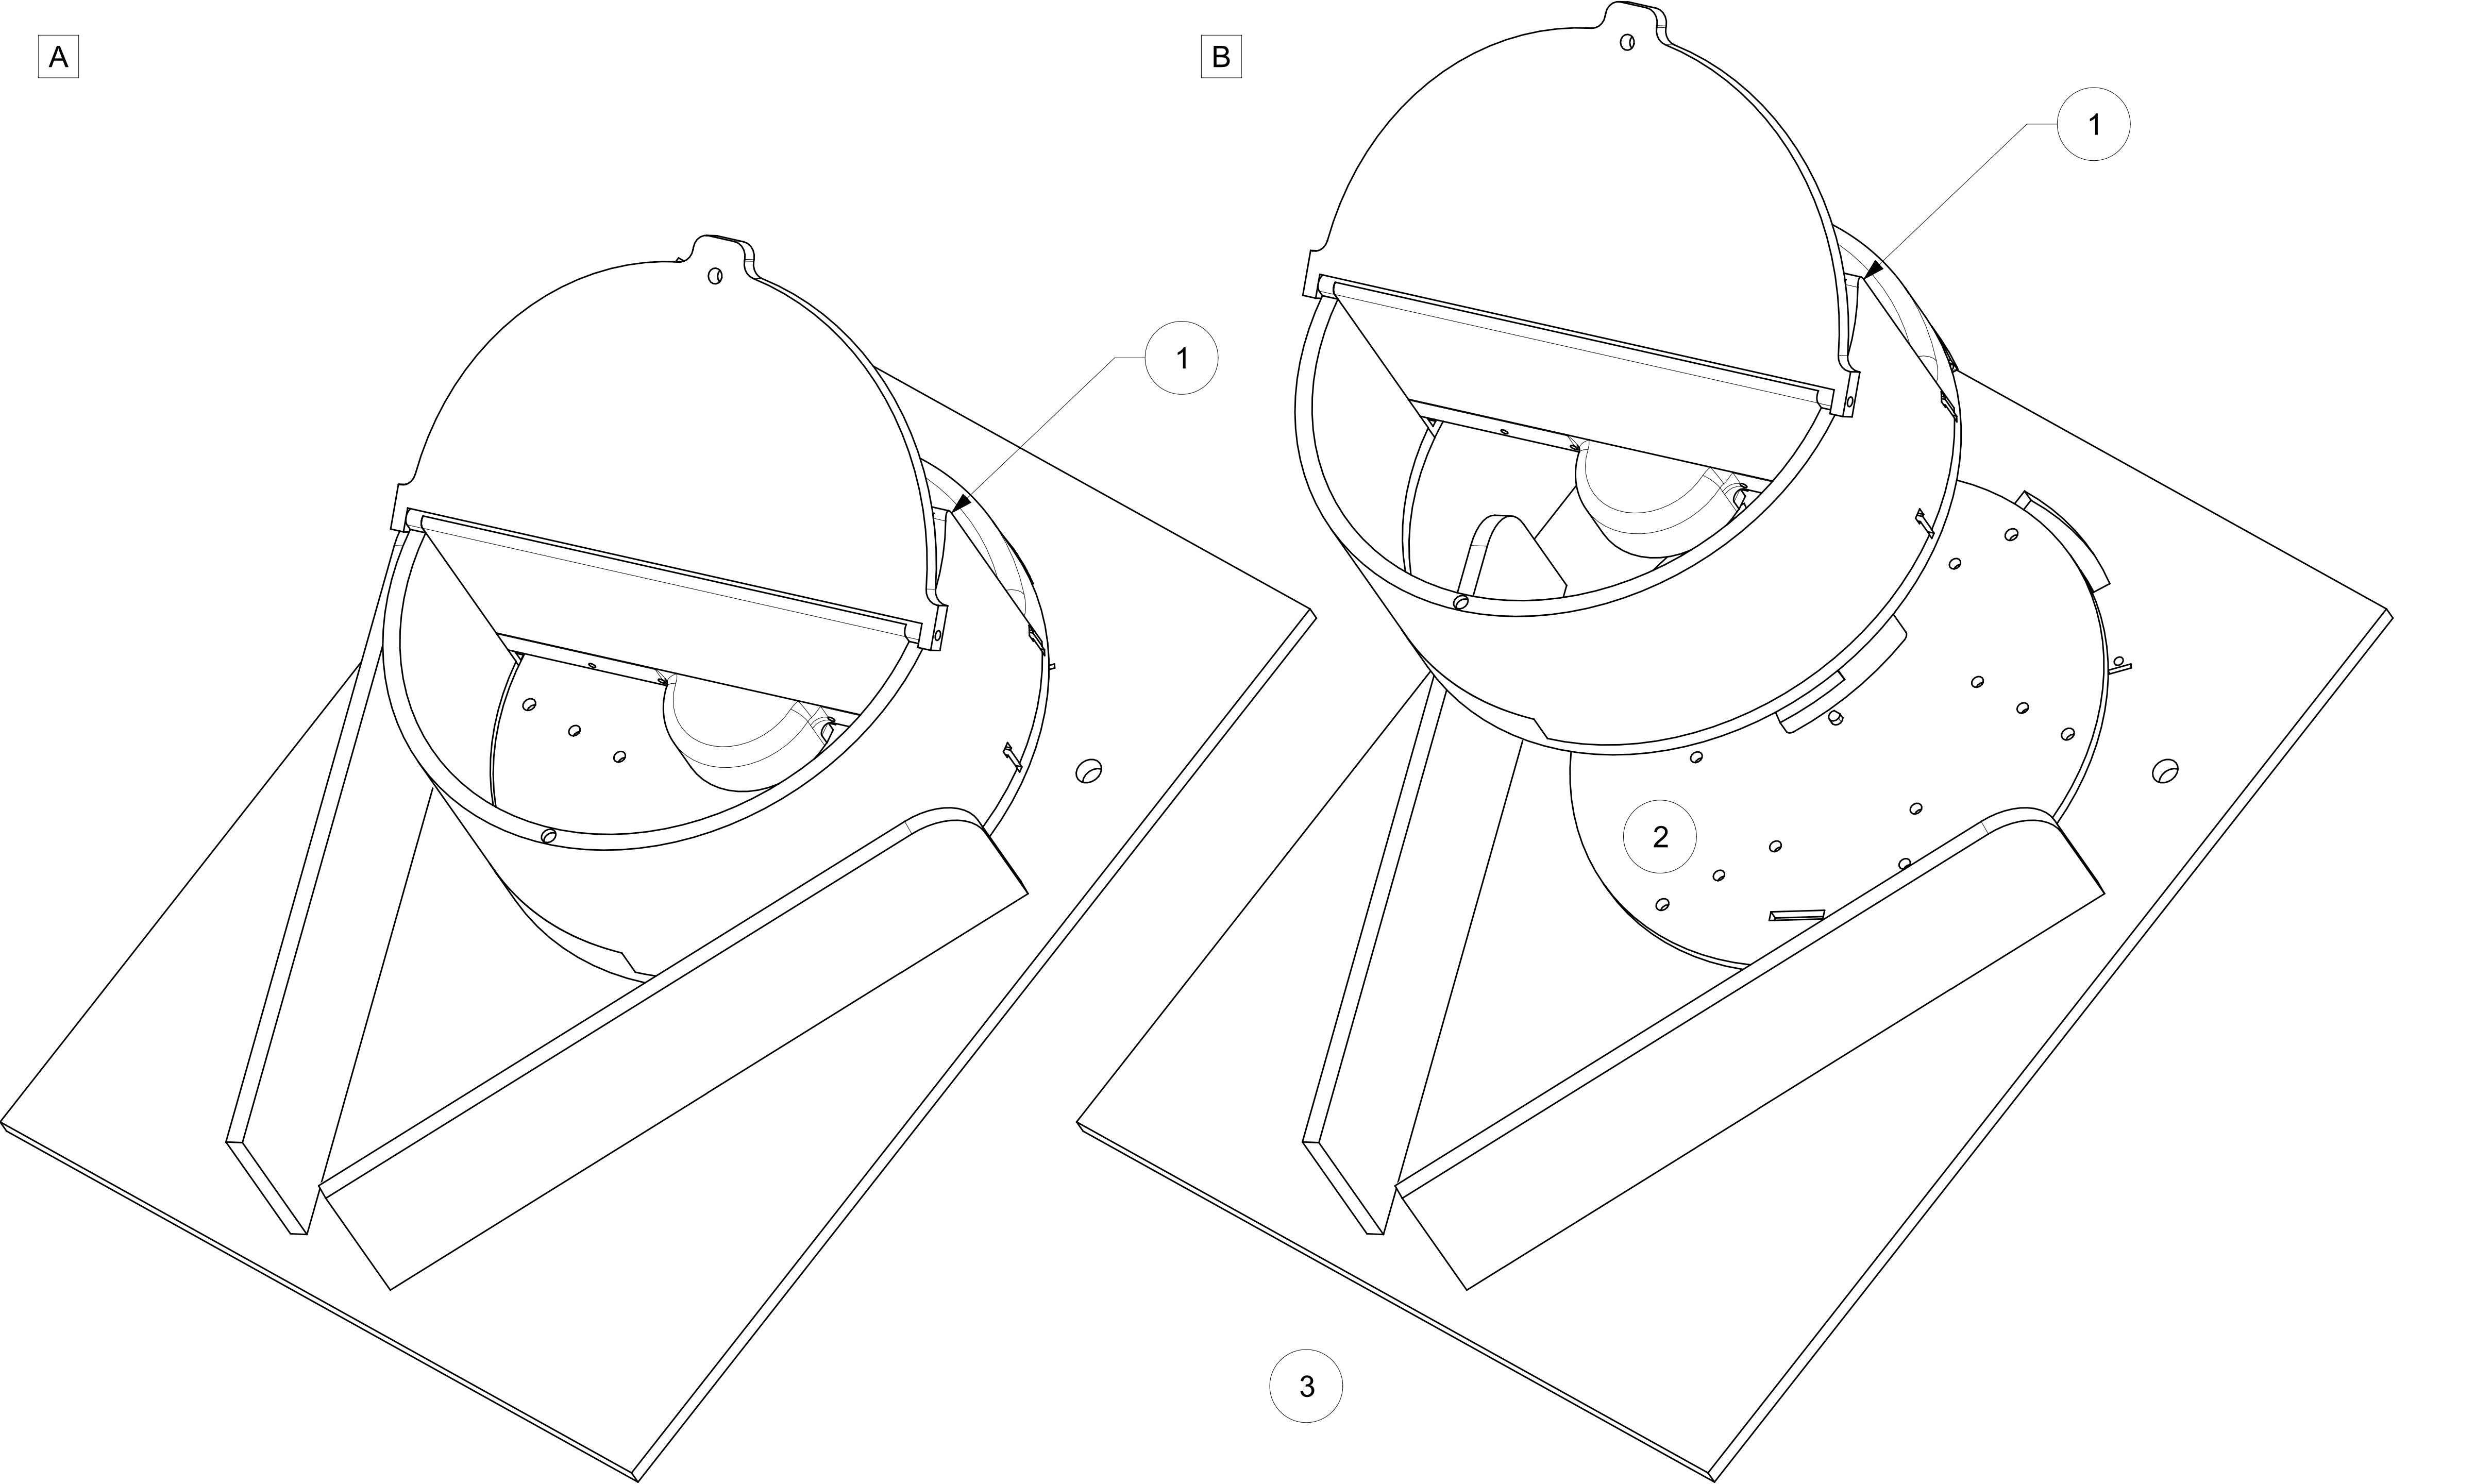
\includegraphics[scale=0.42]{Illustrationen/6-Umsetzung/vereinzelung_entleeren.jpg}
	\caption{Entleerung der Trommel}
	\label{fig:vereinzelung_entleeren}
	\end{figure}
\textbf{Lochmaske}
\newline
Der Funktionsnachweis hat gezeigt, dass das Scheitern der Vereinzelung meist durch das Hängenbleiben der NemaCaps an der Lochmaske verursacht wird. Die Zuverlässigkeit dieser Funktion hängt direkt von den Eigenschaften der Lochmaske ab. Die Materialwahl sowie Fertigungsqualität von diesem Teil ist entscheidend. 
\newline
Folgende Massnahmen werden umgesetzt:
\begin{itemize}
	\item \textbf{Materialwahl:} Die Wahl des passenden Materials mit der geringsten Adhäsion wurde mittels praktischen Tests am 26.4.2017 durchgeführt. Dabei wurden gängige laserbare Materialien (Aluminium, Plexiglas und MDF) miteinander verglichen. Die Tests zeigen, dass Aluminium die geringste Adhäsion gegenüber von NemaCaps aufweist, gefolgt von Plexiglas. Mit MDF wurde die grösste Adhäsion festgestellt, was durch die erhöhte Pulveraufnahme sowie die rauhere Oberfläche zu erklären ist. 
	Die höchste Zufriedenstellung wird mit Aluminium erreicht, wobei die Reibung zwischen Lochmaske und Grundplatte noch nicht berücksichtigt ist. Bei zu hoher Reibung kann auf Plexiglas ausgewichen werden.
	
	\item \textbf{Fertigungsqualität:} Die Tests vom 26.4.2017 zeigten auch, dass die Rauheit der Oberfläche relevant ist. Je feiner die Oberfläche der Bohrung (Punkt 13 in Abbildung \ref{fig:detail_lochmaske}), desto geringer ist das Risiko, dass NemaCaps hängenbleiben. Somit werden diese Löcher nach der Bohrung zusätzlich mit einer Reibale (\textbf{H7?}) ausgerieben. Der ideale Durchmesser D1 muss während der Inbetriebnahme durch zielgerichtetes Ausprobieren erörtert werden.
	
	\item \textbf{Fertigungsverfahren:} Gegeben durch den einfachen zweidimensionalen Aufbau wird die Lochmaske \textbf{mit dem Laser hergsetellt (korrekt?)}. Als Dicke bietet sich 4mm an, sodass ein grosses NemaCap Platz findet und weitere abgestreift werden.
\end{itemize}
Desweiteren ist die Lochmaske mit zwei Langlöchern (14) ausgestattet. Diese werden zur Einpassung von Dauermagneten verwendet, welche zur Positionsbestimmung der Lochmaske dienen. Konstruktiv ist hinzuzufügen, dass der Abstand B in Abbildung \ref{fig:detail_lochmaske} gegeben ist durch die Dimensionen der Schlauchkupplungen (Punkt 8 in Abb. \ref{fig:details_vereinzelung}).
	\begin{figure}[H]
	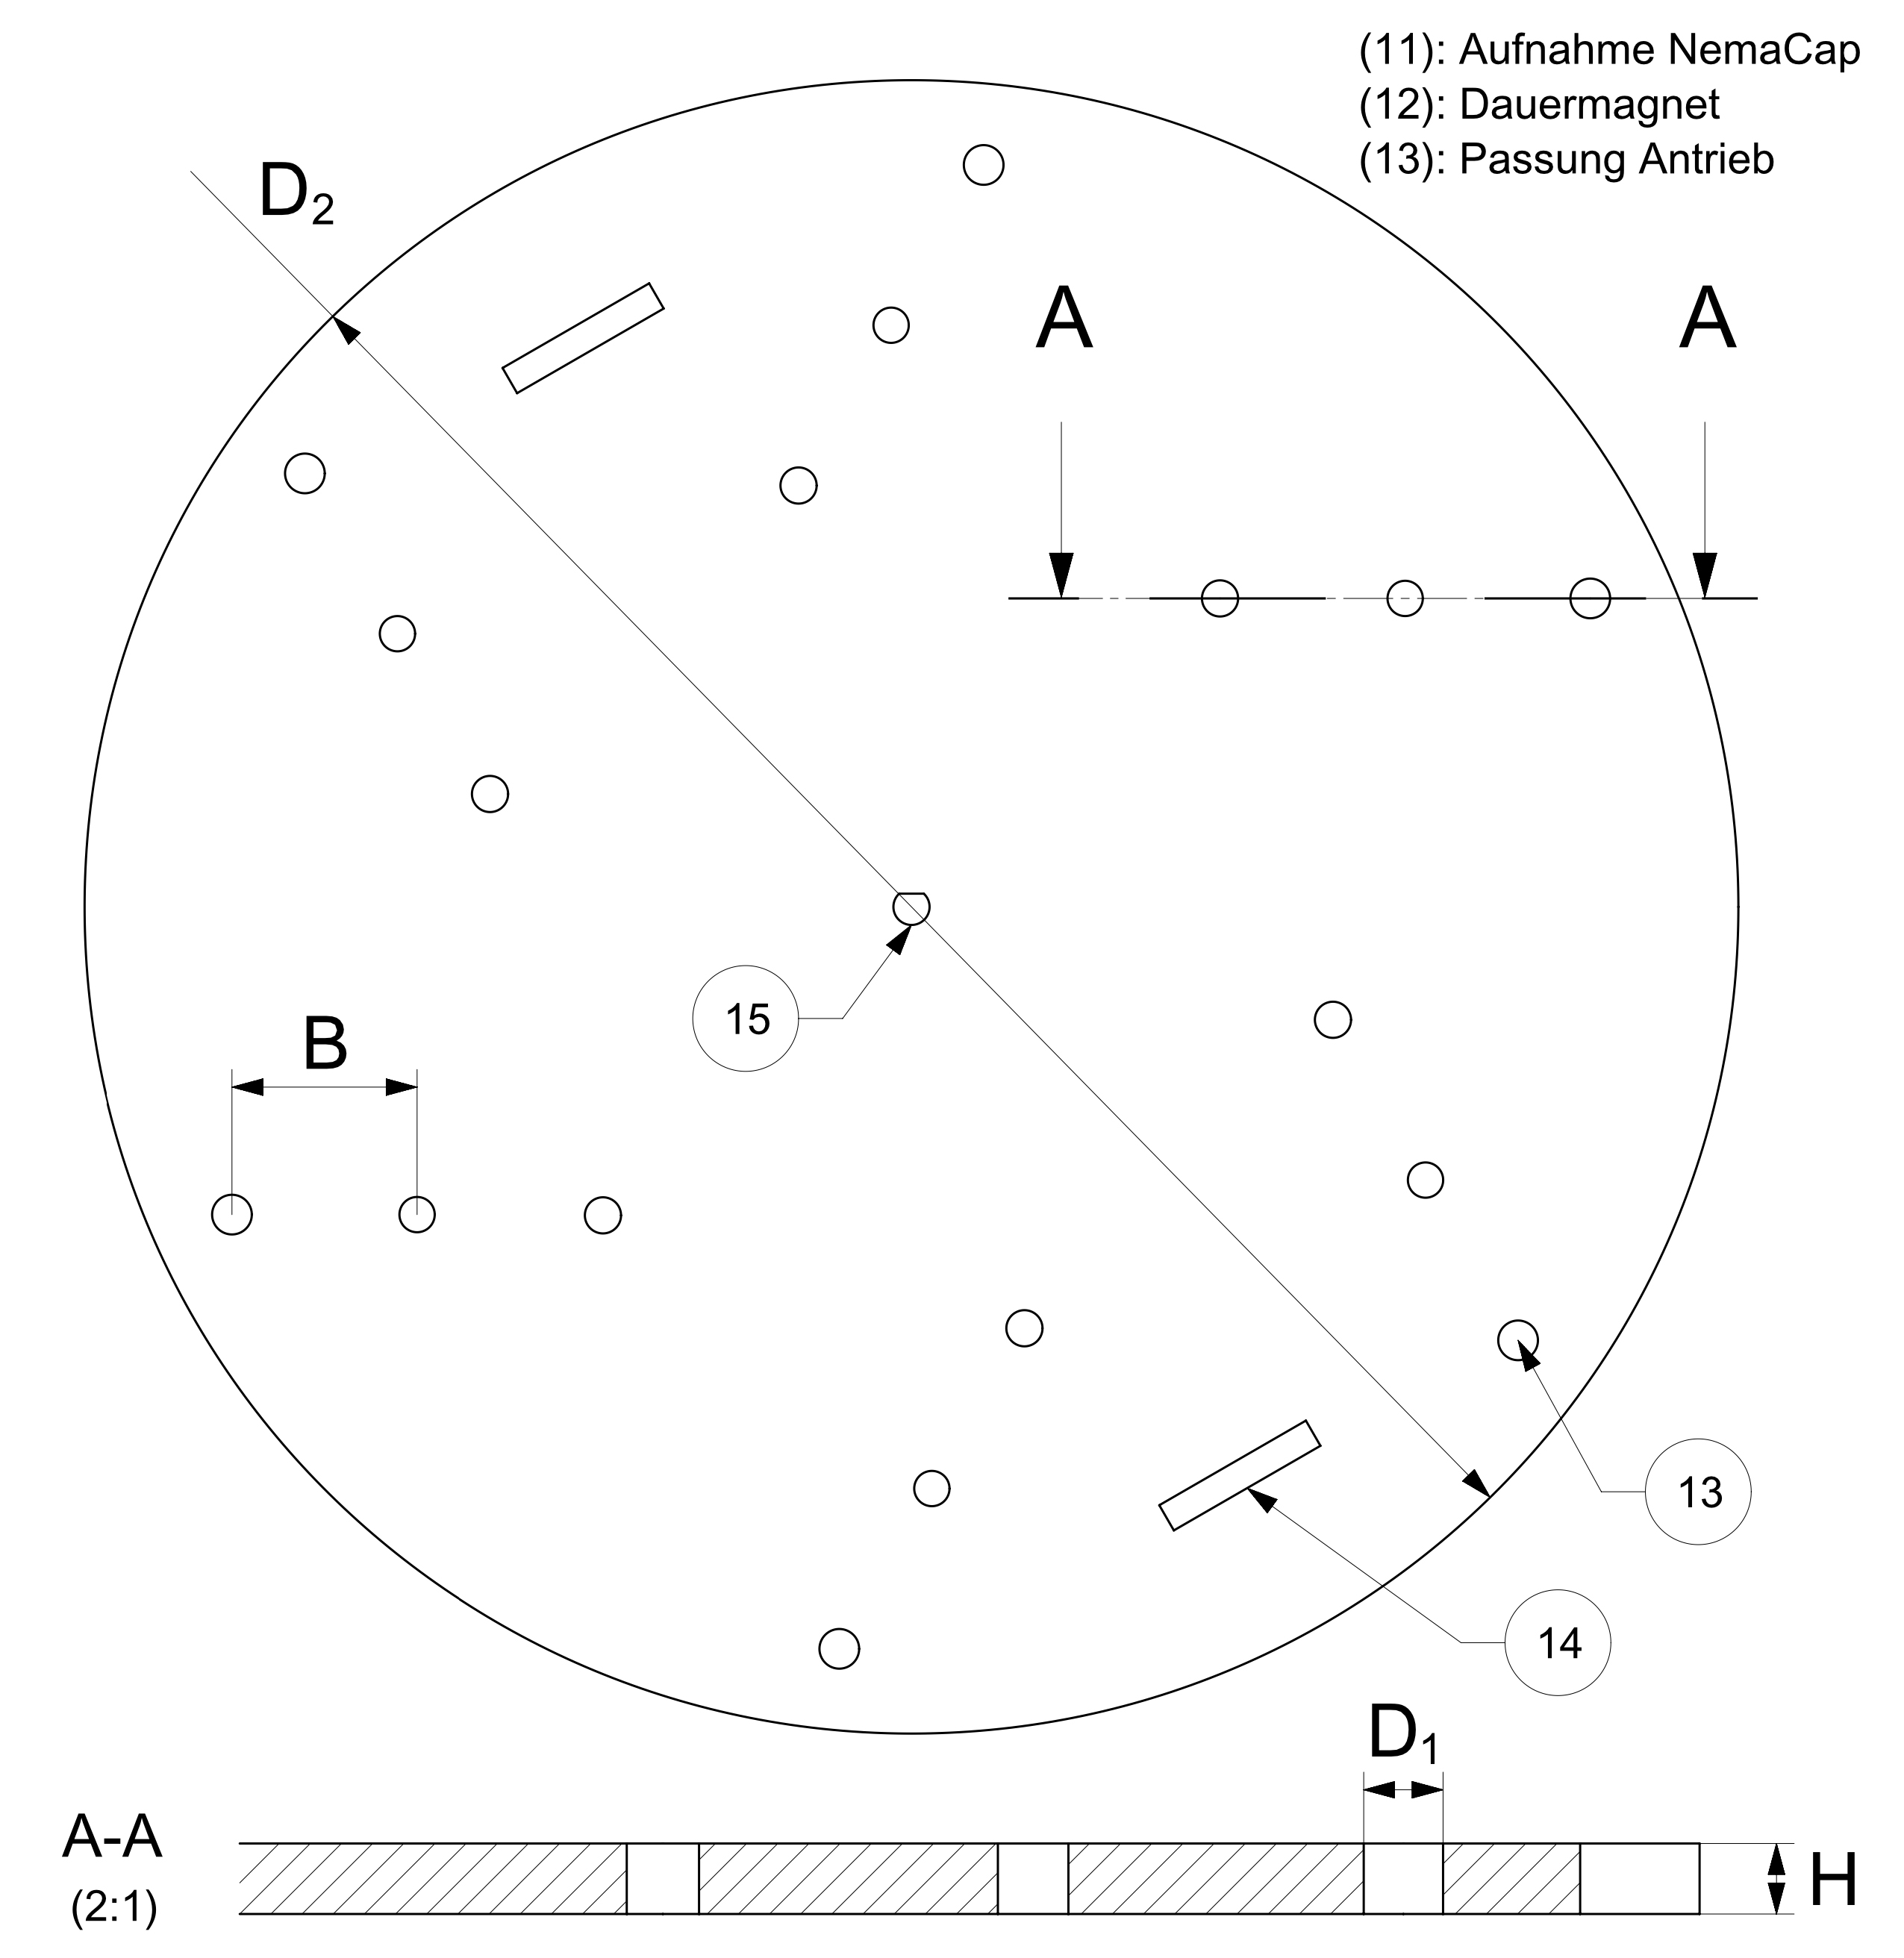
\includegraphics[scale=0.65]{Illustrationen/6-Umsetzung/detail_lochmaske.jpg}
	\caption{Grundriss der Lochmaske mit Schnitt}
	\label{fig:detail_lochmaske}
	\end{figure}
\textbf{Fertigungsverfahren und Materialwahl}
\newline
 Die Grundplatte sowie die Lochmaske werden mit dem Laser gefertigt. Dieses Fertigungsverfahren ist optimal für die Herstellung von zweidimensionalen Teilen. Ein Minimum von verschiedenen Blechdicken spart Umrüstungzeiten und senkt dadurch Kosten. Ein weiterer Vorteil ist, dass ein direkter Export der Fertigungsunterlagen aus dem CAD möglich ist. Für weitere Komponenten anderer Teilfunktionen wird die Realisation aus gelasertem Blech bevorzugt.
\newline
\newline
Die Vereinigung von verschiedensten Funktionen in der Trommel (Integralbauweise) führt zu einer komplexeren Geometrie. Fertigungstechnisch sind gewisse Geometrien konventionell nicht herstellbar. Daher bietet sich Rapid Prototyping als Fertigungsverfahren an. Dadurch ergibt sich jedoch eine Einschränkung: Der Aussendurchmesser der Trommel darf maximal 200mm betragen, da der Bauraum des internen 3D-Druckers 200mm x 200mm x 300mm beträgt. 
\subsection{Setzeinheit}
Die Setzeinheit bezeichnet alle Teile, welche durch die Translation bewegt werden. Auch zur Setzeinheit gehören die Spindel sowie der Spindelantrieb, welche die Translation umsetzen.
\newline
Die wesentlichen Komponenten der Setzeinheit sind in Abbildung \ref{fig:setzeinheit} dargestellt. Dabei wird in diesem Unterkapitel ausschliesslich auf die Komponenten der Setzeinheit eingegangen. Alle Komponenten die zur Verstellung des Topfradius dienen, sind in der Abb.  \ref{fig:setzeinheit} unter Punkt 6 (Verstellmechanik) gesammelt und werden im Kapitel \ref{subsec:Verstellmechanik} näher erläutert.
\newline
\newline
\textbf{Aufbau}
\newline
Die Spindel ist durch eine bewegte Montageplatte (Punkt. 15 in Abb. \ref{fig:setzeinheit}) und drei Führungen (5) mit der Verstellmechanik (7) verbunden. Diese Führungen werden durch drei Gleitlager (6)  an einer Montageplatte (13) gelagert. die zwei oberen Montageplatten (11, 12) dienen zur Montage des Spindelantriebes sowie zur Lagerung der Spindel (4). Um eine weitere Montageplatte zu sparen, ist der Spindelantrieb mittels einer Distanzhülse (2) mit der obersten Montageplatte (11) verbunden. Die unterste Montageplatte (14) dient zur Lagerung der Verstellmechanik sowie zum einfachen Schutz der Mechanik vor Topferde. Dadurch ist gewährleistet das nur ein minimaler Teil (der Stechdorn, 8) der bewegten Komponenten in Kontakt mit der Topferde kommt.
	\begin{figure}[H]
	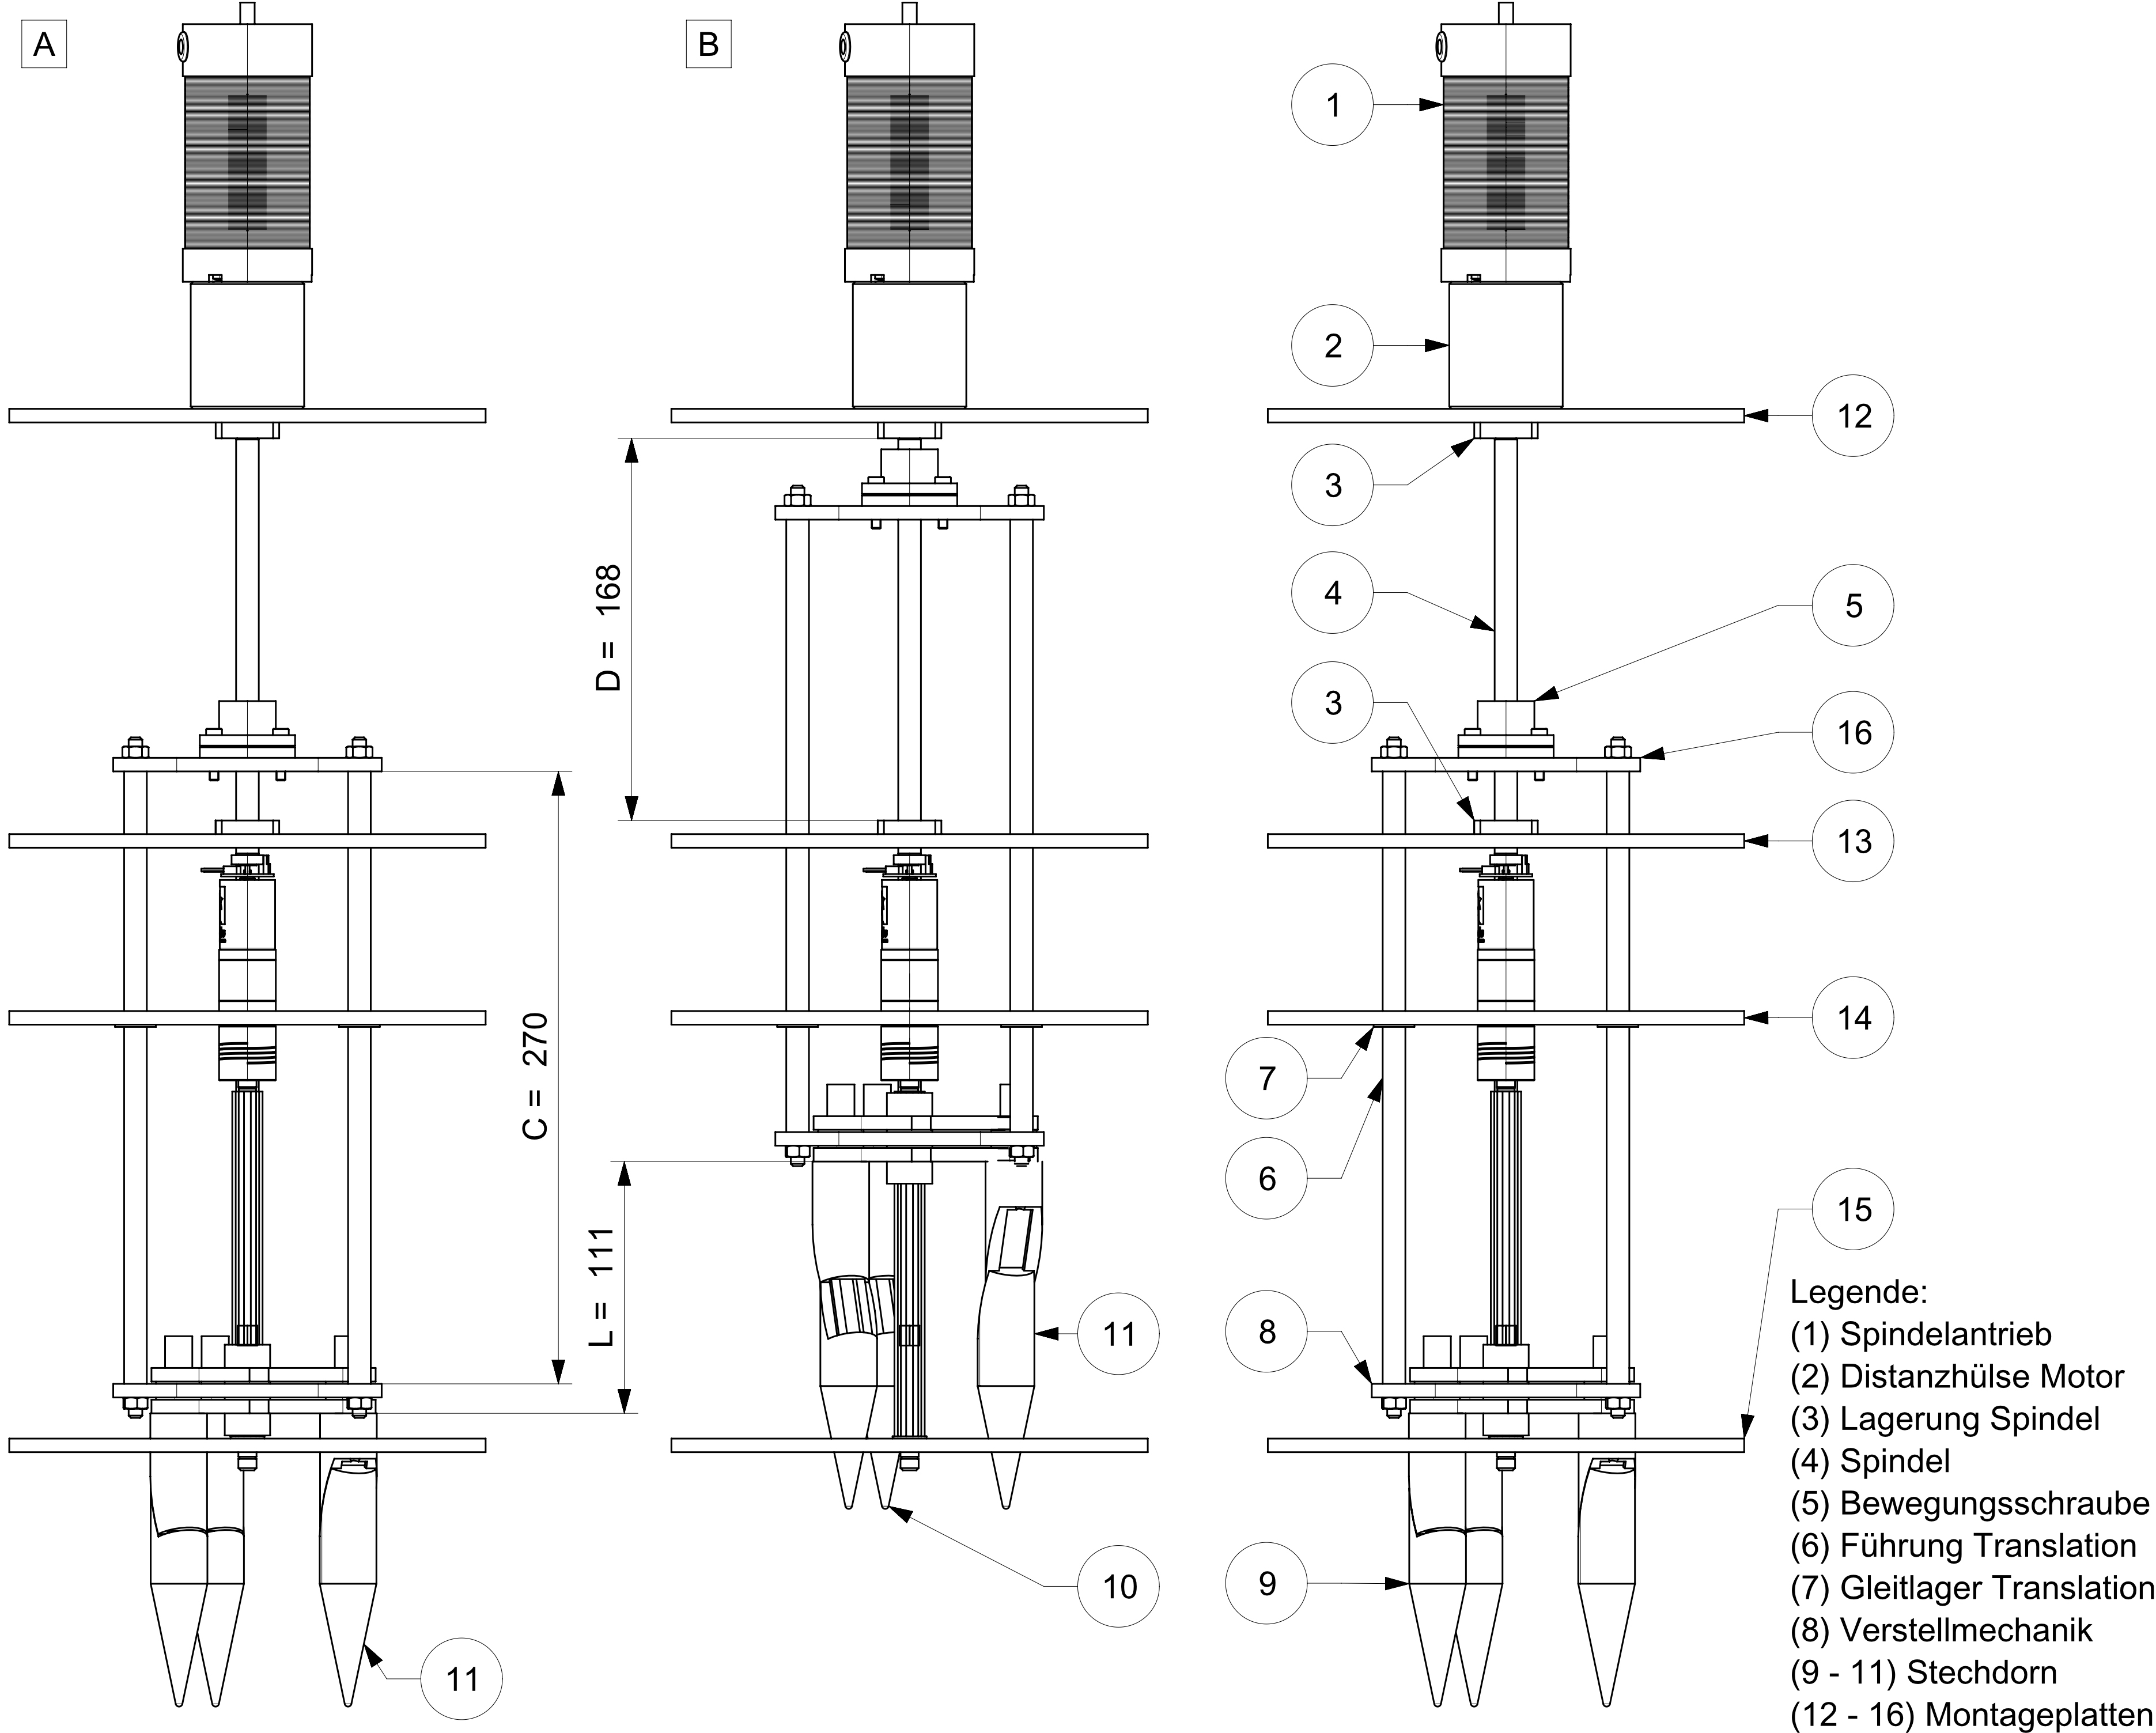
\includegraphics[scale=0.53]{Illustrationen/6-Umsetzung/setzeinheit_aio.jpg}
	\caption{Detaillierte Übersicht der Setzeinheit}
	\label{fig:setzeinheit}
\end{figure}

 
\subsubsection{Translation der Setzeinheit}
Die Setzeinheit macht folgenden Bewegungsablauf, um drei NemaCaps in einen Topf zu pflanzen:
\begin{itemize}
	\item \textbf{A - Setzloch ausheben:} Die Spindel bewegt die Setzeinheit nach unten und treibt den Stechdorn in die Erde. Dadurch verschliesst sich der Stechdorn (Punkt 9 in Abb. \ref{fig:setzeinheit}). 

	\item \textbf{B - NemaCap setzen:} Nachdem die Erde verdrängt und das Setzloch ausgehoben ist, bewegt sich die Setzeinheit wieder nach oben. Nun öffnet sich der Stechdorn (10) indem sich der untere Teil durch die Schwerkraft auf die Seite bewegt. So können die NemaCaps in das ausgehobene Setzloch fallen.
\end{itemize}

Konstruktiv sind drei Masse hervor zu heben:
\begin{itemize}
	\item \textbf{L - Maximaler Hubweg:} Der maximale Hub L beträgt 111mm. Gemäss Berechnungen (\textbf{Siehe Anhang XY}) muss dieser mindestens 86mm betragen. Somit beträgt die Reserve 25mm. 
	
	\item \textbf{C - Länge der Führungen:} Die Länge der Führungen ist gegeben durch den Hubweg L, die Höhe des Motors für die Verstellmechanik dessen Kupplung. Dies bedingt eine Länge von 270mm.
	
	\item \textbf{D - Länge der Spindel:} Die Spindellänge ist gegeben durch den maximalen Hub L, der Höhe der Bewegungsschraube sowie die Montageplatte.
\end{itemize}
\textbf{Lagerung}
\newline
Die Lagerung der translatorischen Bewegung wird durch drei Gleitlager (Punkt. 6 in Abb. \ref{fig:setzeinheit}) realisiert. Dabei werden diese in die Montageplatte (12) eingepresst. Dafür werden drei Kunststoff Gleitlager iglidur J3FM-1012 von igus verwendet. Begründet wird die Wahl dadurch, dass Kunstoffgleitlager schmiermittel- und wartungsfrei sind, geringe Reibwerte und eine hohe Lebensdauer aufweisen. Weiter sind dies Standard-Maschinenelemente und dadurch günstig erhätlich. Weitere Informationen die Gleitlager sind aus dem Datenblatt zu entnehmen.
\newline
\textbf{Kinetik?}
\newline
\textbf{Knickgefahr?}
\newline

\subsubsection{Spindel}
Die Wahl der Spindel und des Spindelantriebes haben einen entscheidenden Einfluss auf die Erfüllung des Setzprozesses innerhalb der vorgegeben Zeit. Parameter wie Steigung, Spindeldurchmesser und Material der Spindel wirken sich direkt auf die Massenträgheit und somit auf das erforderliche Beschleunigungsmoment aus.
 \\
 \newline
\textbf{Auslegung und Wahl}
 \\
Die Subkapitel befasst sich mit der Auslegung und Berechnung der Spindel. Dabei sind Berechnungen in zusammengefasster Form dargestellt. Der vollständige Rechenweg und die detailierte Vorgehensweise sind im Anhang (\textbf{Datei XY}) zu entnehmen.

Gegeben durch den Setzprozess und die Geometrie sind folgende Daten:
	\begin{figure}[H]
	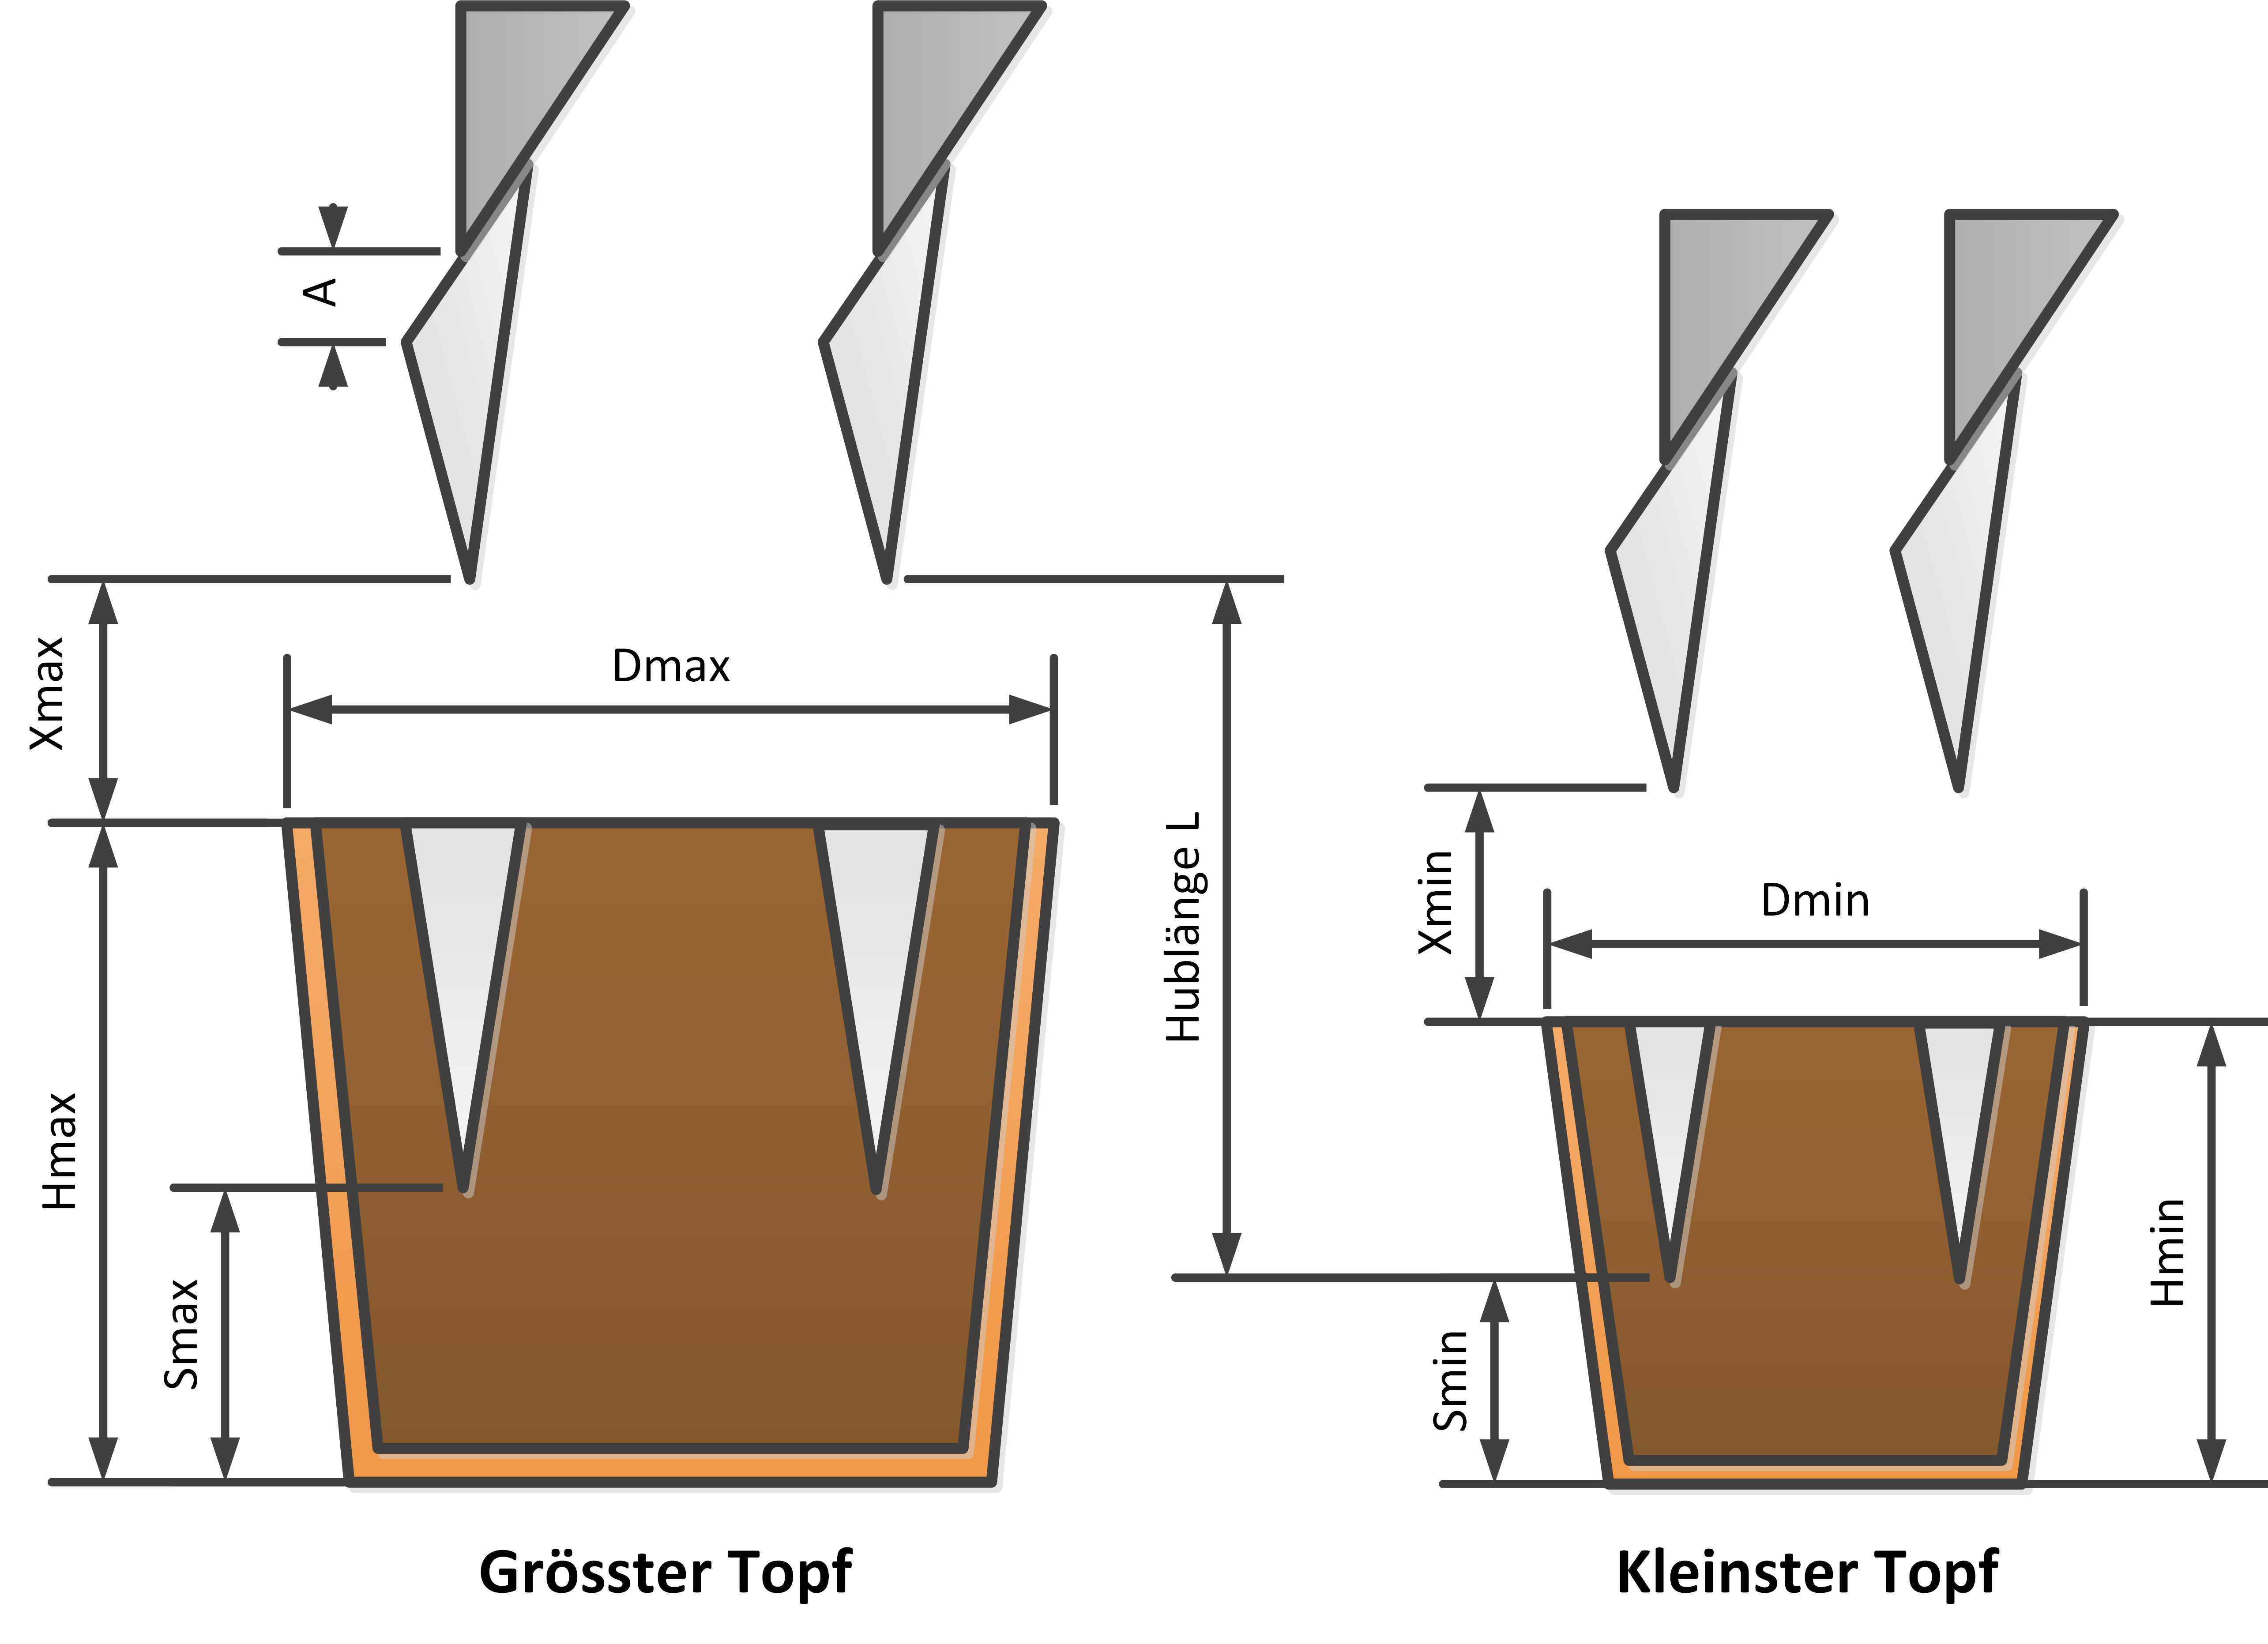
\includegraphics[width=1\textwidth]{Illustrationen/6-Umsetzung/topfgeometrie.png}
	\caption{Geometrie der Töpfe und des Setzprozess}
	\label{fig:topfgeometrie}
	\end{figure}
\begin{table}[H]
\begin{tabular}{|l|c|c|l|}
	\hline 
	& Grösster Topf (max) & Kleinster Topf (min) & Kommentar \\ 
	\hline 
	Durchmesser D [mm] & 140 & 90 & Aus Datenblatt \\ 
	\hline 
	Höhe h [mm] & 106 & 67 & Aus Datenblatt \\ 
	\hline 
	max. Einsetztiefe S [mm] & 63.6 & 40.2 & 0.6 x Höhe \\ 
	\hline 
	Sicherheitsabstand X [mm] & 15 & 15 & Annahme \\ 
	\hline 
	Ausfahrlänge A Dorn [mm] & 15 & 15 & Annahme \\ 
	\hline 
\end{tabular} 
	\caption{Randbedingungen für Spindelauslegung}
	\label{tab:Randbedingungen}
\end{table}

Anhand dieser Randbedingungen und den getroffenen Annahmen ergibt sich eine Beschleunigungs- und Bremszeit tb=0.1125s. Bei einem maximalen Hubweg Umax = 72.4mm beträgt die grösste durschnittliche Geschwindigkeit vavmax:

\begin{equation}
v_{avmax}=\frac{U_{max}}{t_{b}}=\frac{72.4mm}{0.1125s}=643.5mm/s
\end{equation}
\newline
Die Geschwindigkeit des Dornes kann streng idealisiert gemäss Abbildung XY dargestellt werden:
	\begin{figure}[H]
	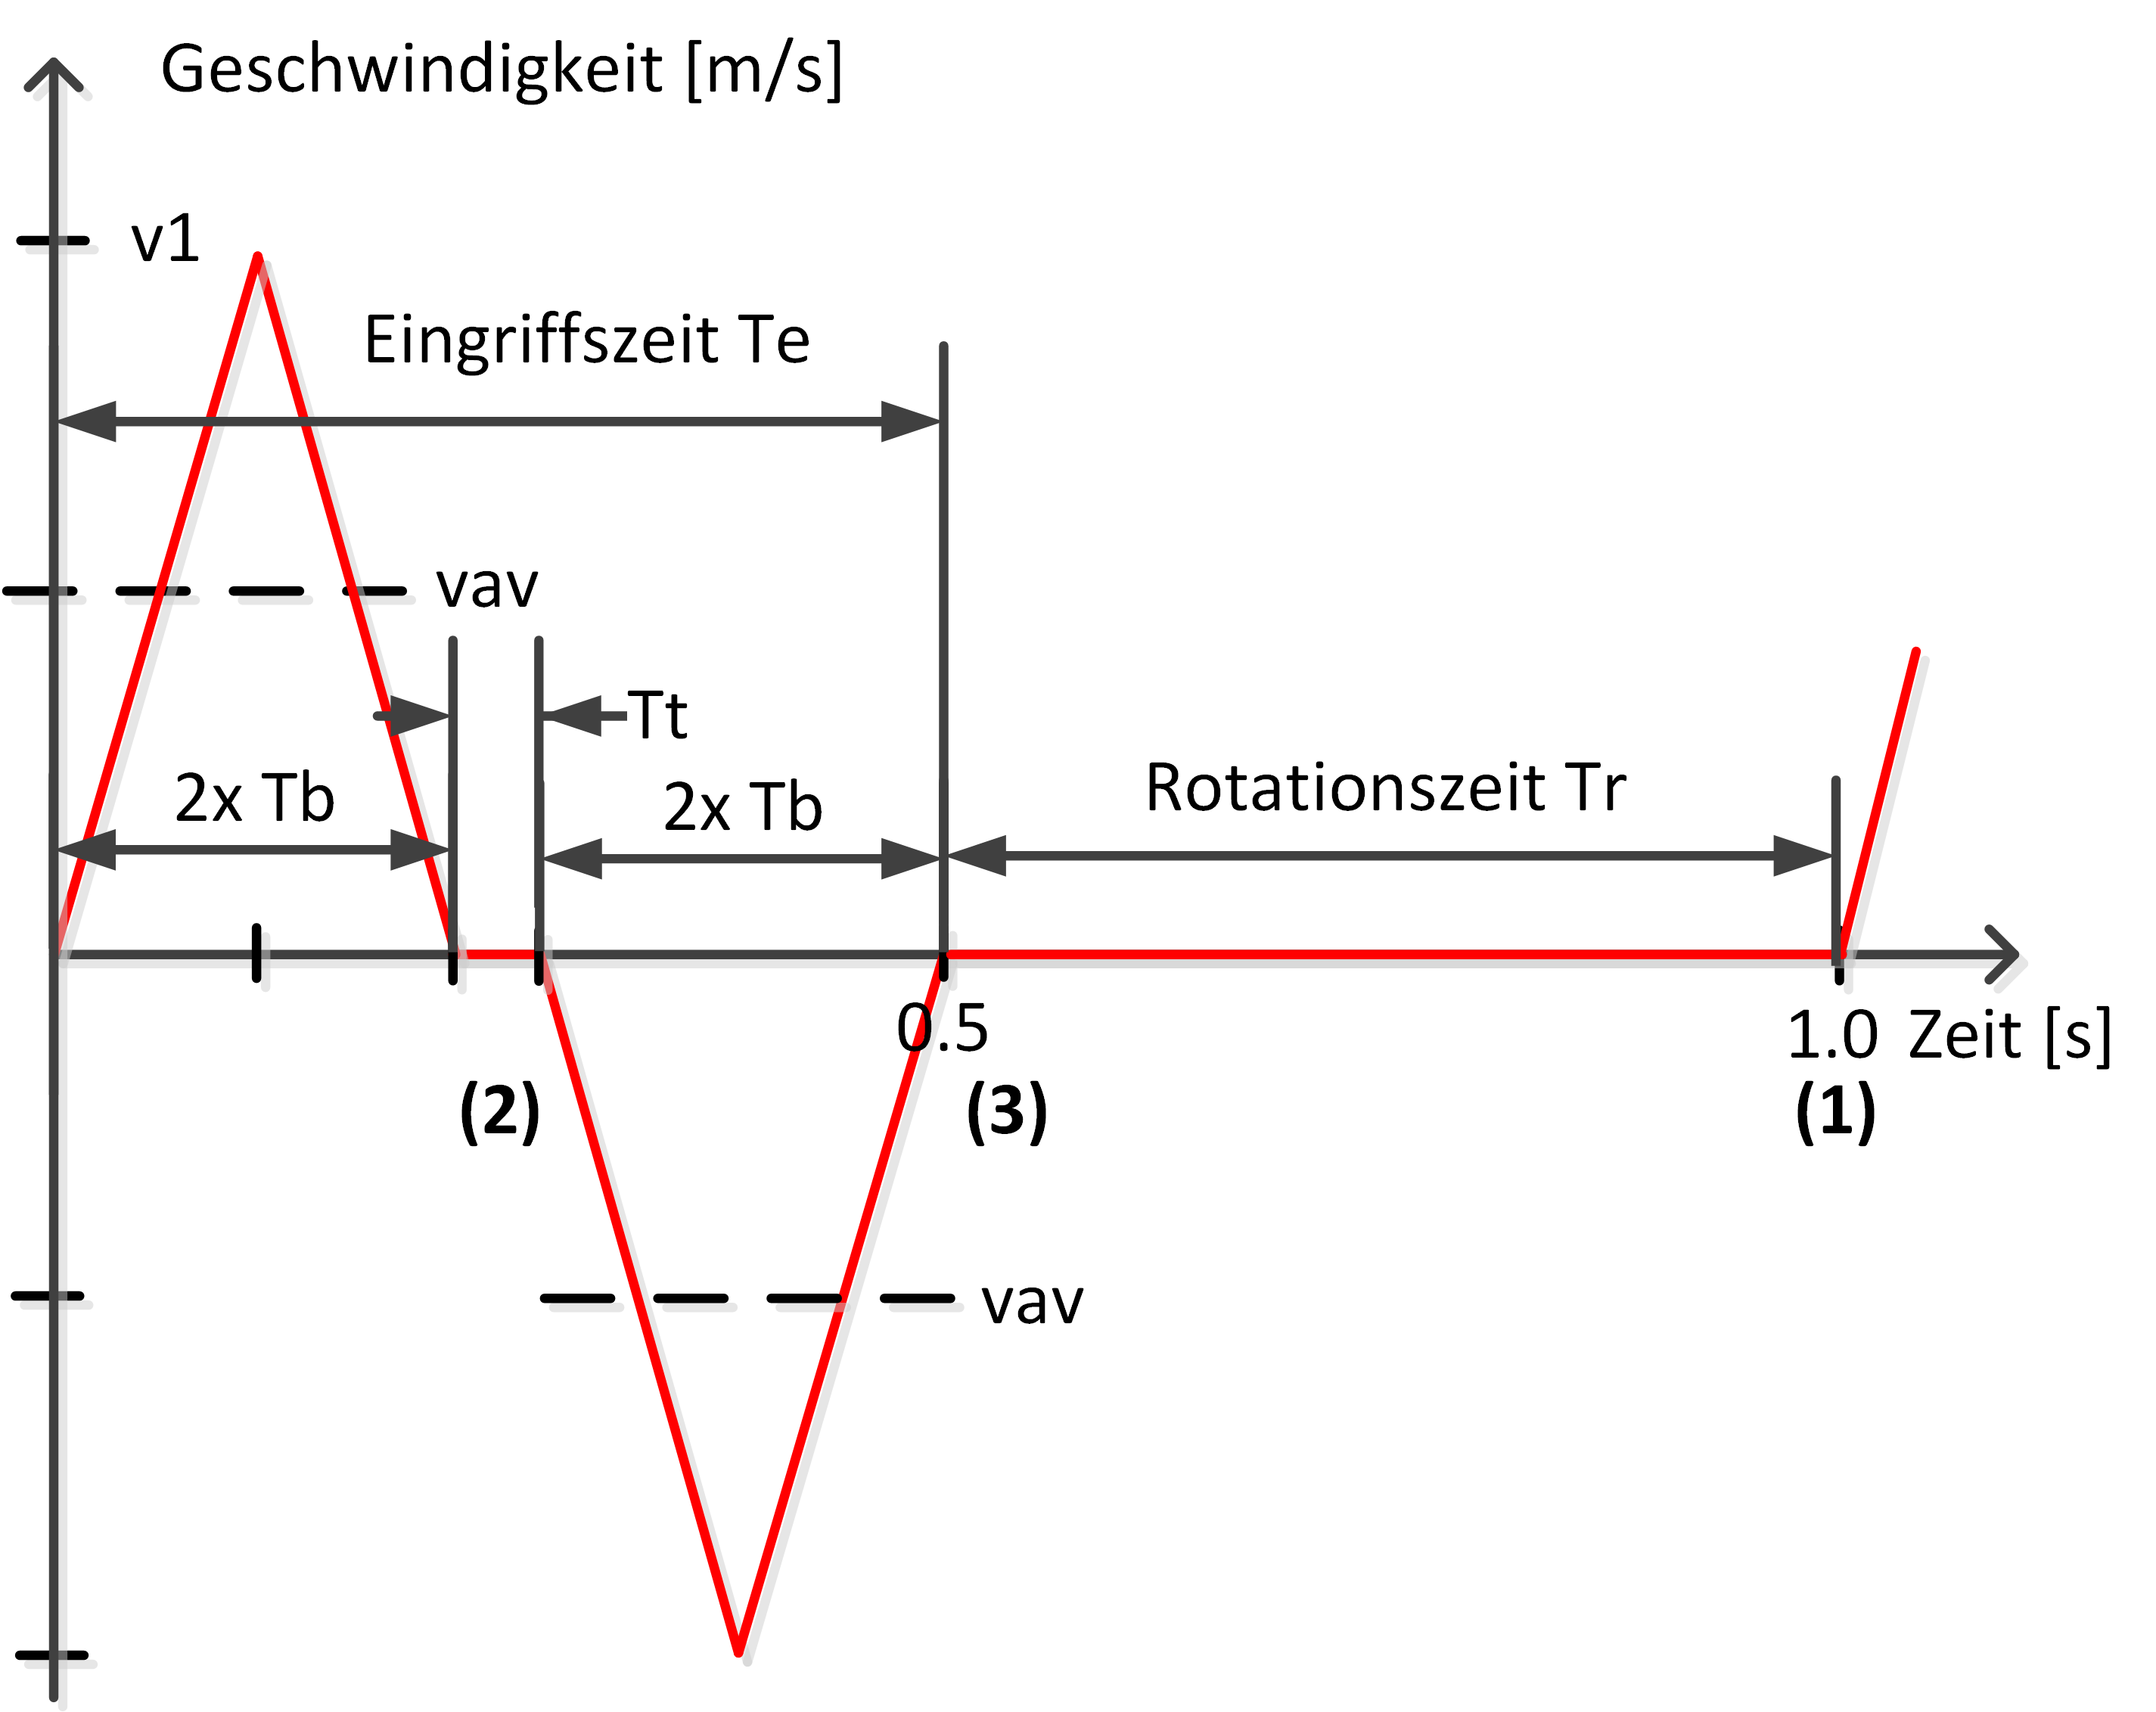
\includegraphics[width=1\textwidth]{Illustrationen/6-Umsetzung/vprofil_dorn.png}
	\caption{Geschwindigkeitsprofil des Dorns}
	\label{fig:vprofil_dorn}
\end{figure}
Orientiert an den Anforderungen aus Kapitel \ref{subsec:Translation} und der berechneten Geschwindigkeit sind vier Steilgewindespindeln von Igus ausgewählt worden. In Rücksprache mit Mark Chalençon, Produktmanager bei igus Schweiz GmbH, wurde die Auswahl der Produkte zusätzlich verifiziert (Mail vom 18.4.17).
\begin{table}[H]
\begin{tabular}{|c|c|}
	\hline 
	Ds14x30 (Edelstahl) & Ds10x25 (Edelstahl) \\ 
	\hline 
	Ds14x30 (Aluminium) & Ds10x25 (Aluminium) \\ 
	\hline 
\end{tabular} 
\caption{Ausgewählte Steilgewindespindeln von Igus}
\label{tab:spindeln}
\end{table}
Mit diesen Angaben kann die Spindel durch ein reduziertes Model dargestellt werden, analog zu Abbildung 13-5, S.448 \cite{roloffmatek}:
 	\begin{figure}[H]
 	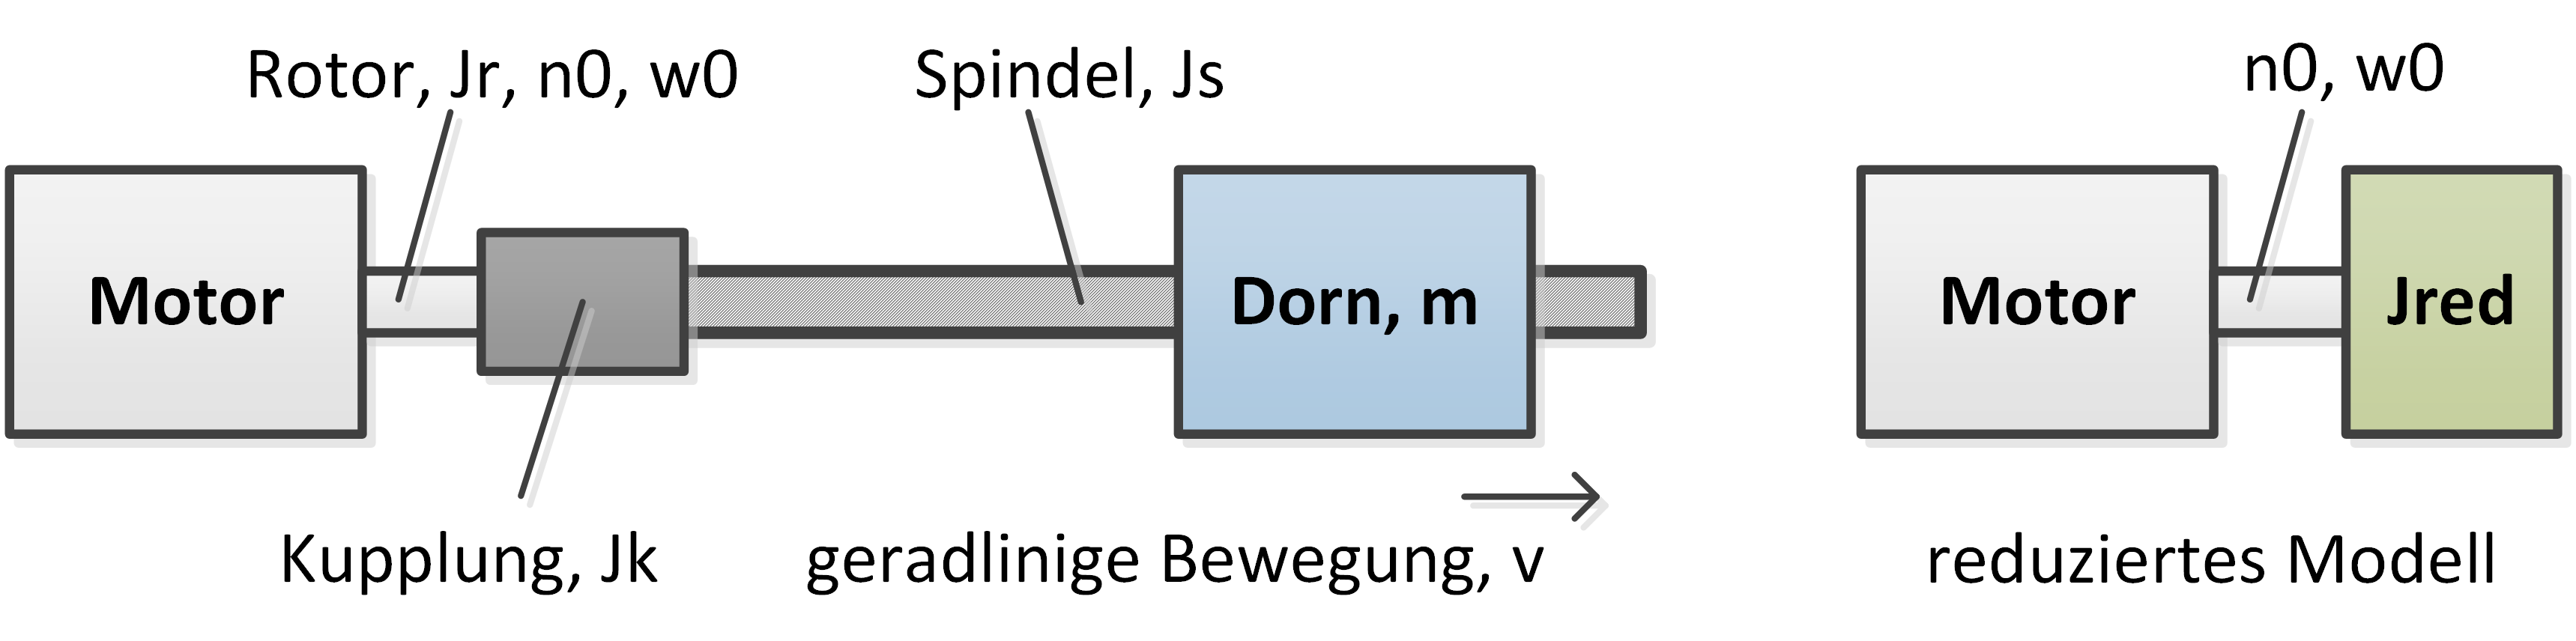
\includegraphics[width=1\textwidth]{Illustrationen/6-Umsetzung/red_modell.png}
 	\caption{Schema des Spindelantriebs sowie des reduzierten Modells}
 	\label{fig:red_modell}
	\end{figure}
wobei für das reduzierte Modell sich die reduzierte Massenträgheit Jred und das benötigte Beschleunigungsmoment Ma ergibt (Gleichung 13.3 und 13.4, S.449):
\begin{equation}
J_{red}=J_{rotor}+J_{kupplung}+J_{spindel}+m*(\frac{v_{1}}{w_{v1}})^{2}
\end{equation}
\begin{equation}
M_{a}=J_{red}*\frac{w_{2}-w_{1}}{t_{b}}=J_{red}*\frac{w_{v1}}{t_{b}}
\end{equation}
Für die ausgewählten Spindeltypen ergibt dies folgende Werte:
\newline
\textbf{Tabelle der Spindeln}
Die berechneten Werte für das Beschleunigungsmoment Ma aus \textbf{Tabelle XY} zeigen, dass sich alle ausgewählten Spindeln für den evaluierten Spindelantrieb eignen.
\newline
\newline

Als definitive Wahl wird die Spindel Ds10x25 aus Edelstahl ausgewählt. Folgende Argumente sind ausschlaggebend:
	\begin{itemize}
	\item Die Variante Ds10x25 aus Edelstahl bietet das Optimum von geringem Durchmesser und hoher Festigkeit. Das leicht höhere Beschleunigungsmoment der Ds10x25 aus Edelstahl zur Ds14x30 wird für eine höhere Festigkeit in Kauf genommen.
	
	\item \ Die geringere Steigung gibt dem Motor mehr Weg (Umdrehungen) zur Beschleunigung.
\end{itemize}
\textbf{Lagerung und Kupplung der Spindel}
\newline
Die Spindel wird durch ein Fest- sowie ein Loslager eindeutig gelagert. Das Festlager ist in der obersten Montageplatte (Punkt. 11 in Abb. \ref{fig:setzeinheit}) vorgesehen, das Loslager in der zweiten Montageplatte (12). Diese Anordnung ist bewusst so gewählt, sodass das Festlager Axialkräfte aufnimmt und Spindelantrieb axial unbelastet bleibt. Für die Lagerung werden fertige Lagerböcke von Mädler Norm-Antrieb AG verwendet, welche speziell für Spindeln ausgelegt sind. Diese sind einfach im Einbau und erfordern keinen zusätzlichen Entwicklungsaufwand. An der Spindel wird konstruktiv einen Freistich Form E gemäss Normen-Auszug umgesetzt (\textbf{Siehe Zeichnung XY})\cite{vsm}.
\newline
Zur mechanischen Verbindung zwischen Spindelantrieb und Spindel wird eine drehstarre Kupplung verwendet. Dadurch kann eine winkelgetreue Drehmomentenübertragung gewährleistet werden, was für diese Anwendung essentiell ist. Hierfür wird die Kupplung HELICAL WA 20-8-6 aus Aluminium von Ringspann AG verwendet. Die Wahl eines kleinen Aussendurchmessers (20mm) und eine leichter Werkstoff sind für ein möglichst geringes zusätzliches Trägheitsmoment entscheidend und wurde hier berücksichtigt.
\subsubsection{Montage}
Wie schon mehrfach erwähnt werden mehrere verschiedenste Komponenten an Montageplatten montiert. Wie aus Abbildung \ref{fig:setzeinheit} ersichtlich, werden die Montageplatten vertikal angeordnet. Diese Anordnung bildet so das Gerüst für eine funktionierende Setzeinheit. Wie in Kapitel XY erwähnt, bietet sich die konsequente Fertigung mittels Lasermaschine an. Mechanisch fixiert werden die Montageplatten durch Aluminium Profile der Firma Kanya AG (weitere Informationen in \textbf{Kap XY}), wobei durch die Nut der Profile eine Blechdicke von 6mm vorgegeben ist. Diese Konstruktion bringt folgende Vorteile:
	\begin{itemize}
	\item Auf unterschiedlichen Ebenen können so Komponenten angeordnet werden. Das Hinzufügen von weiteren Komponenten ist auf einfachste Art realisierbar. Kommt eine Komponente hinzu, wird die benötigte Kontur (z.B. ein Langloch oder Bohrung) vorgesehen und die Komponente ist montierbar.
	\item Die Fixierung der Montageplatten durch Aluminium-Profile bringt weitere Flexibilität bei der Montage. Dadurch bleibt die Höhe der einzelnen Platten verstellbar. Auch seitlich können die Platten in eine Richtung verstellt werden.
\end{itemize}
 	\begin{figure}[H]
	\includegraphics[width=1\textwidth]{Illustrationen/6-Umsetzung/Montageplatten.png}
	\caption{Übersicht der Montageplatten}
	\label{fig:montageplatten}
\end{figure}
Die Montageplatten 1 bis 3 aus Abbildung \ref{fig:montageplatten} verfügen über drei Langlöcher (Detail A), welche um jeweils 120° verschoben angeordnet sind. Diese sind für die flexible Führung der Schläuche vorgesehen.
\subsection{Verstellmechanik}
\label{verstellmechanik}
Die Hauptaufgabe der Verstellmechanik ist, die automatisierte Einstellung aller geforderten Topfradien. Auch ist die Verstellmechanik Teil der Setzeinheit. Dabei kann keine klare Abgrenzung zur Setzeinheit gemacht werden, da in gewissen Komponenten Funktionen beider Einheiten vereint sind. Auch ist die Verstellmechanik klar an Wunschanforderung formuliert. Die Wunschanforderung birgt einen erhöhten Entwicklungsaufwand. Dies wird bewusst in Kauf genommen, um ein Maximum an Automatisierungsgrad zu erreichen. Möchte trotzdem auf die automatische Verstellung der Topfradien verzichtet werden, ist die Entwicklung der Pflichtanforderung weniger zeitintensiv und rasch implementiert.
\newline
\newline
\textbf{Aufbau}
\newline
Die Konstruktion der Verstellmechanik basiert auf dem erstellten Funktionsmuster. die Grundidee ist, dass über zwei Kulissen (eine radiale und eine lineare) der Topfradius zentral an einer Welle verstellt werden kann. Ein klarer Vorteil ist, dass dadurch nur ein Aktor für die Verstellung aller Stechdorne benötigt wird. Die Konstruktion kann in zwei Teile unterteilt werden:
\begin{itemize}
	\item \textbf{Bewegter Teil}: Dieser Teil wird durch die Spindel bewegt. Die drei Stechdorne (Punkt 4 in Abb. \ref{fig:details_vm}) sind durch zwei Kulissen (2, 3) verstellbar gelagert. Durch die Verbindung Keilnabe (5) - Keilwelle (1) sind diese mit dem unbewegten Teil gekoppelt. Eine geringes Gewicht des bewegten Teils ist für die Beschleunigung dieser Masse essentiell.
	
	\item \textbf{Unbewegter Teil:} Der unbewegte Teil dieser Einheit führt die Verstellung der Topfradien aus. Ein Getriebemotor (8), welcher durch eine Kupplung (9) mit der Keilwelle verbunden ist, führt die Verstellung der Topfradien aus. Diese Umsetzung besticht dadurch, dass anhand der Verbindung Keilnabe (5) - Keilwelle (1) bedeutend weniger Masse an der transaltorischen Bewegung teilnimmt. Dies bringt wertvolle Gewichteinsparnisse.
\end{itemize}
	\begin{figure}[H]
	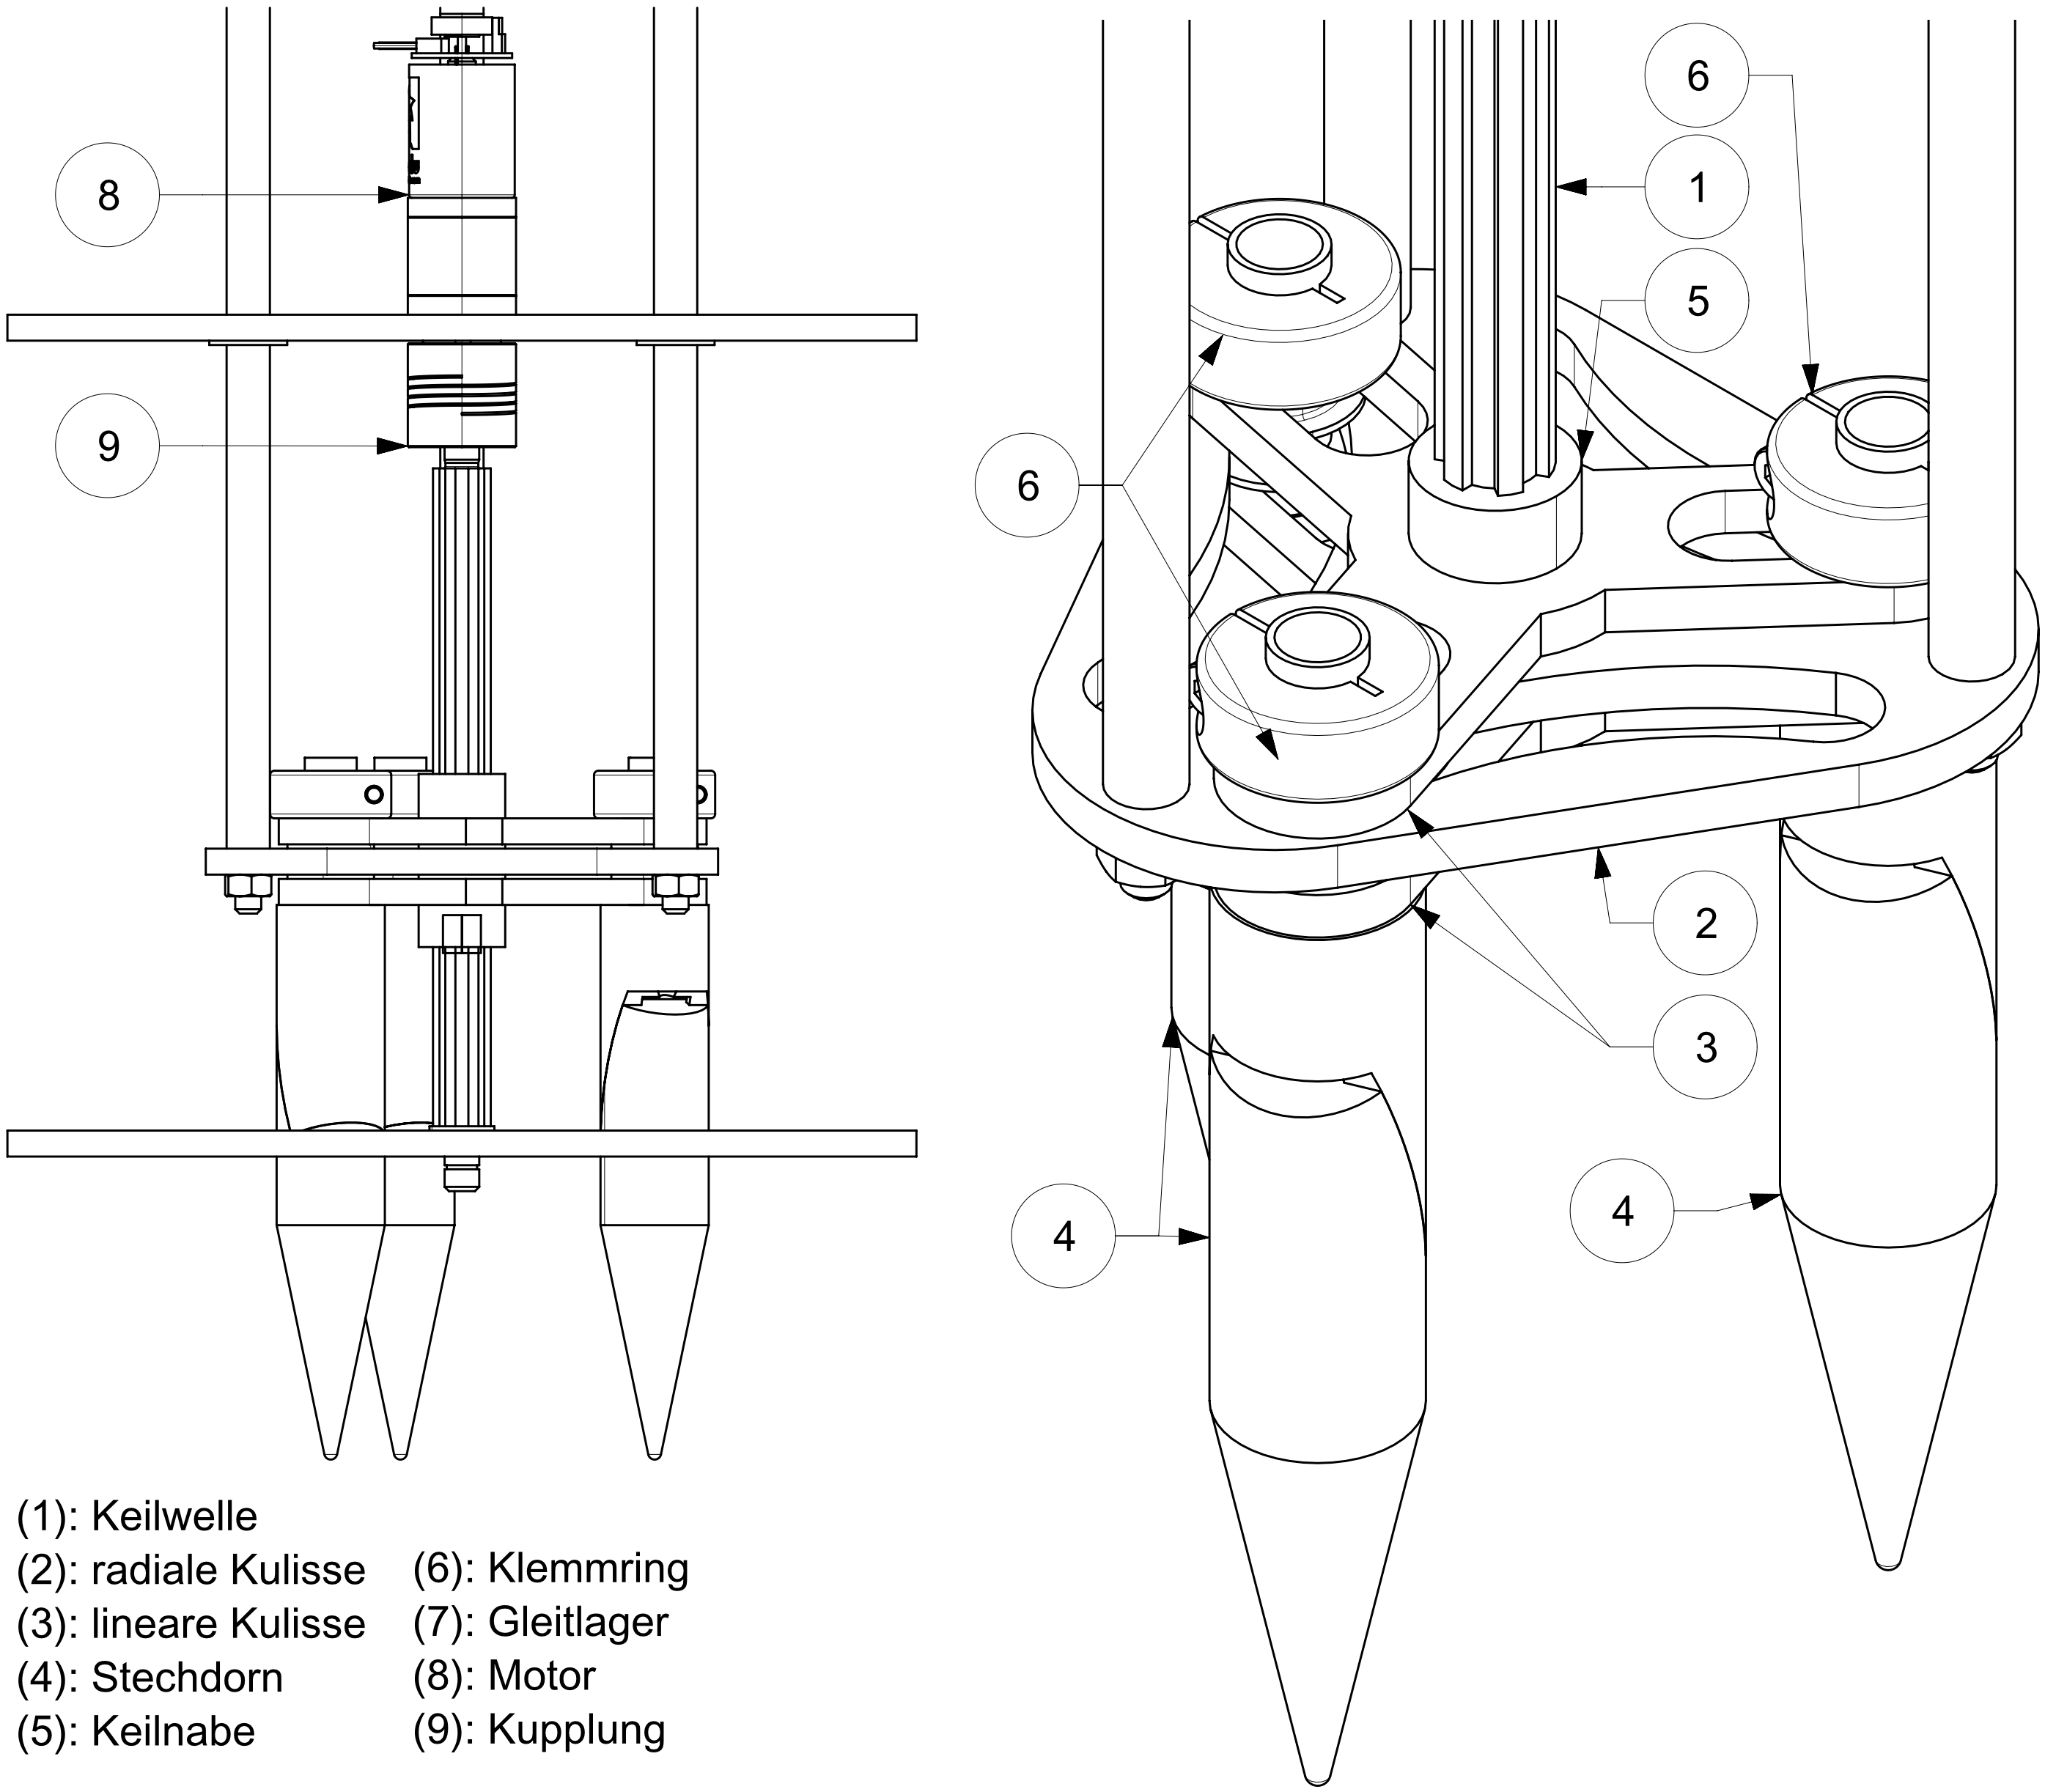
\includegraphics[scale=0.6]{Illustrationen/6-Umsetzung/details_vm.jpg}
	\caption{Detaillierte Übersicht der Verstellmechanik}
	\label{fig:details_vm}
	\end{figure}
Die Lagerung der Keilwelle wird nur wenig beansprucht, da durch die translatorische Freiheit der Keilnabe (entlang der Achse) keine Axialkräfte auftretten. Da die Verstellung des Topfradius nur wenige Male pro Tag vorgenommen wird, kann nach Roloff Matekk (Kapitel 14.3.1) von einer statischen Belastung (da n<10U/min) ausgegangen werden \cite{roloffmatek}. Daher ist die Verwendung eines Gleitlagers am unteren Ende (10) ausreichend. Verwendet wird das Gleitlager idlidur J3 von Igus. Am oberen Ende ist die Keilwelle (1) über die Kupplung (9) durch den Getriebemotor (8) gelagert.
\newline

Der Stechdorn wird durch zwei lineare Kulissen (Punkt 3 in Abb \ref{fig:schnitt_vm}) und eine radiale Kulisse (2) geführt. dabei sind die linearen Kulissen (3) mit der Keilnabe verbunden, die Radiale über die Führungen mit der Spindel. Um die Reibung zwischen Stechdorn und Kulissen zu vermindern werden auch hier Gleitlager (7) von igus eingesetzt. Die ganze Mechanik wird dabei durch die Auflage des Stechdorns (4) und einem Klemmring (6) gehalten.
	\begin{figure}[H]
	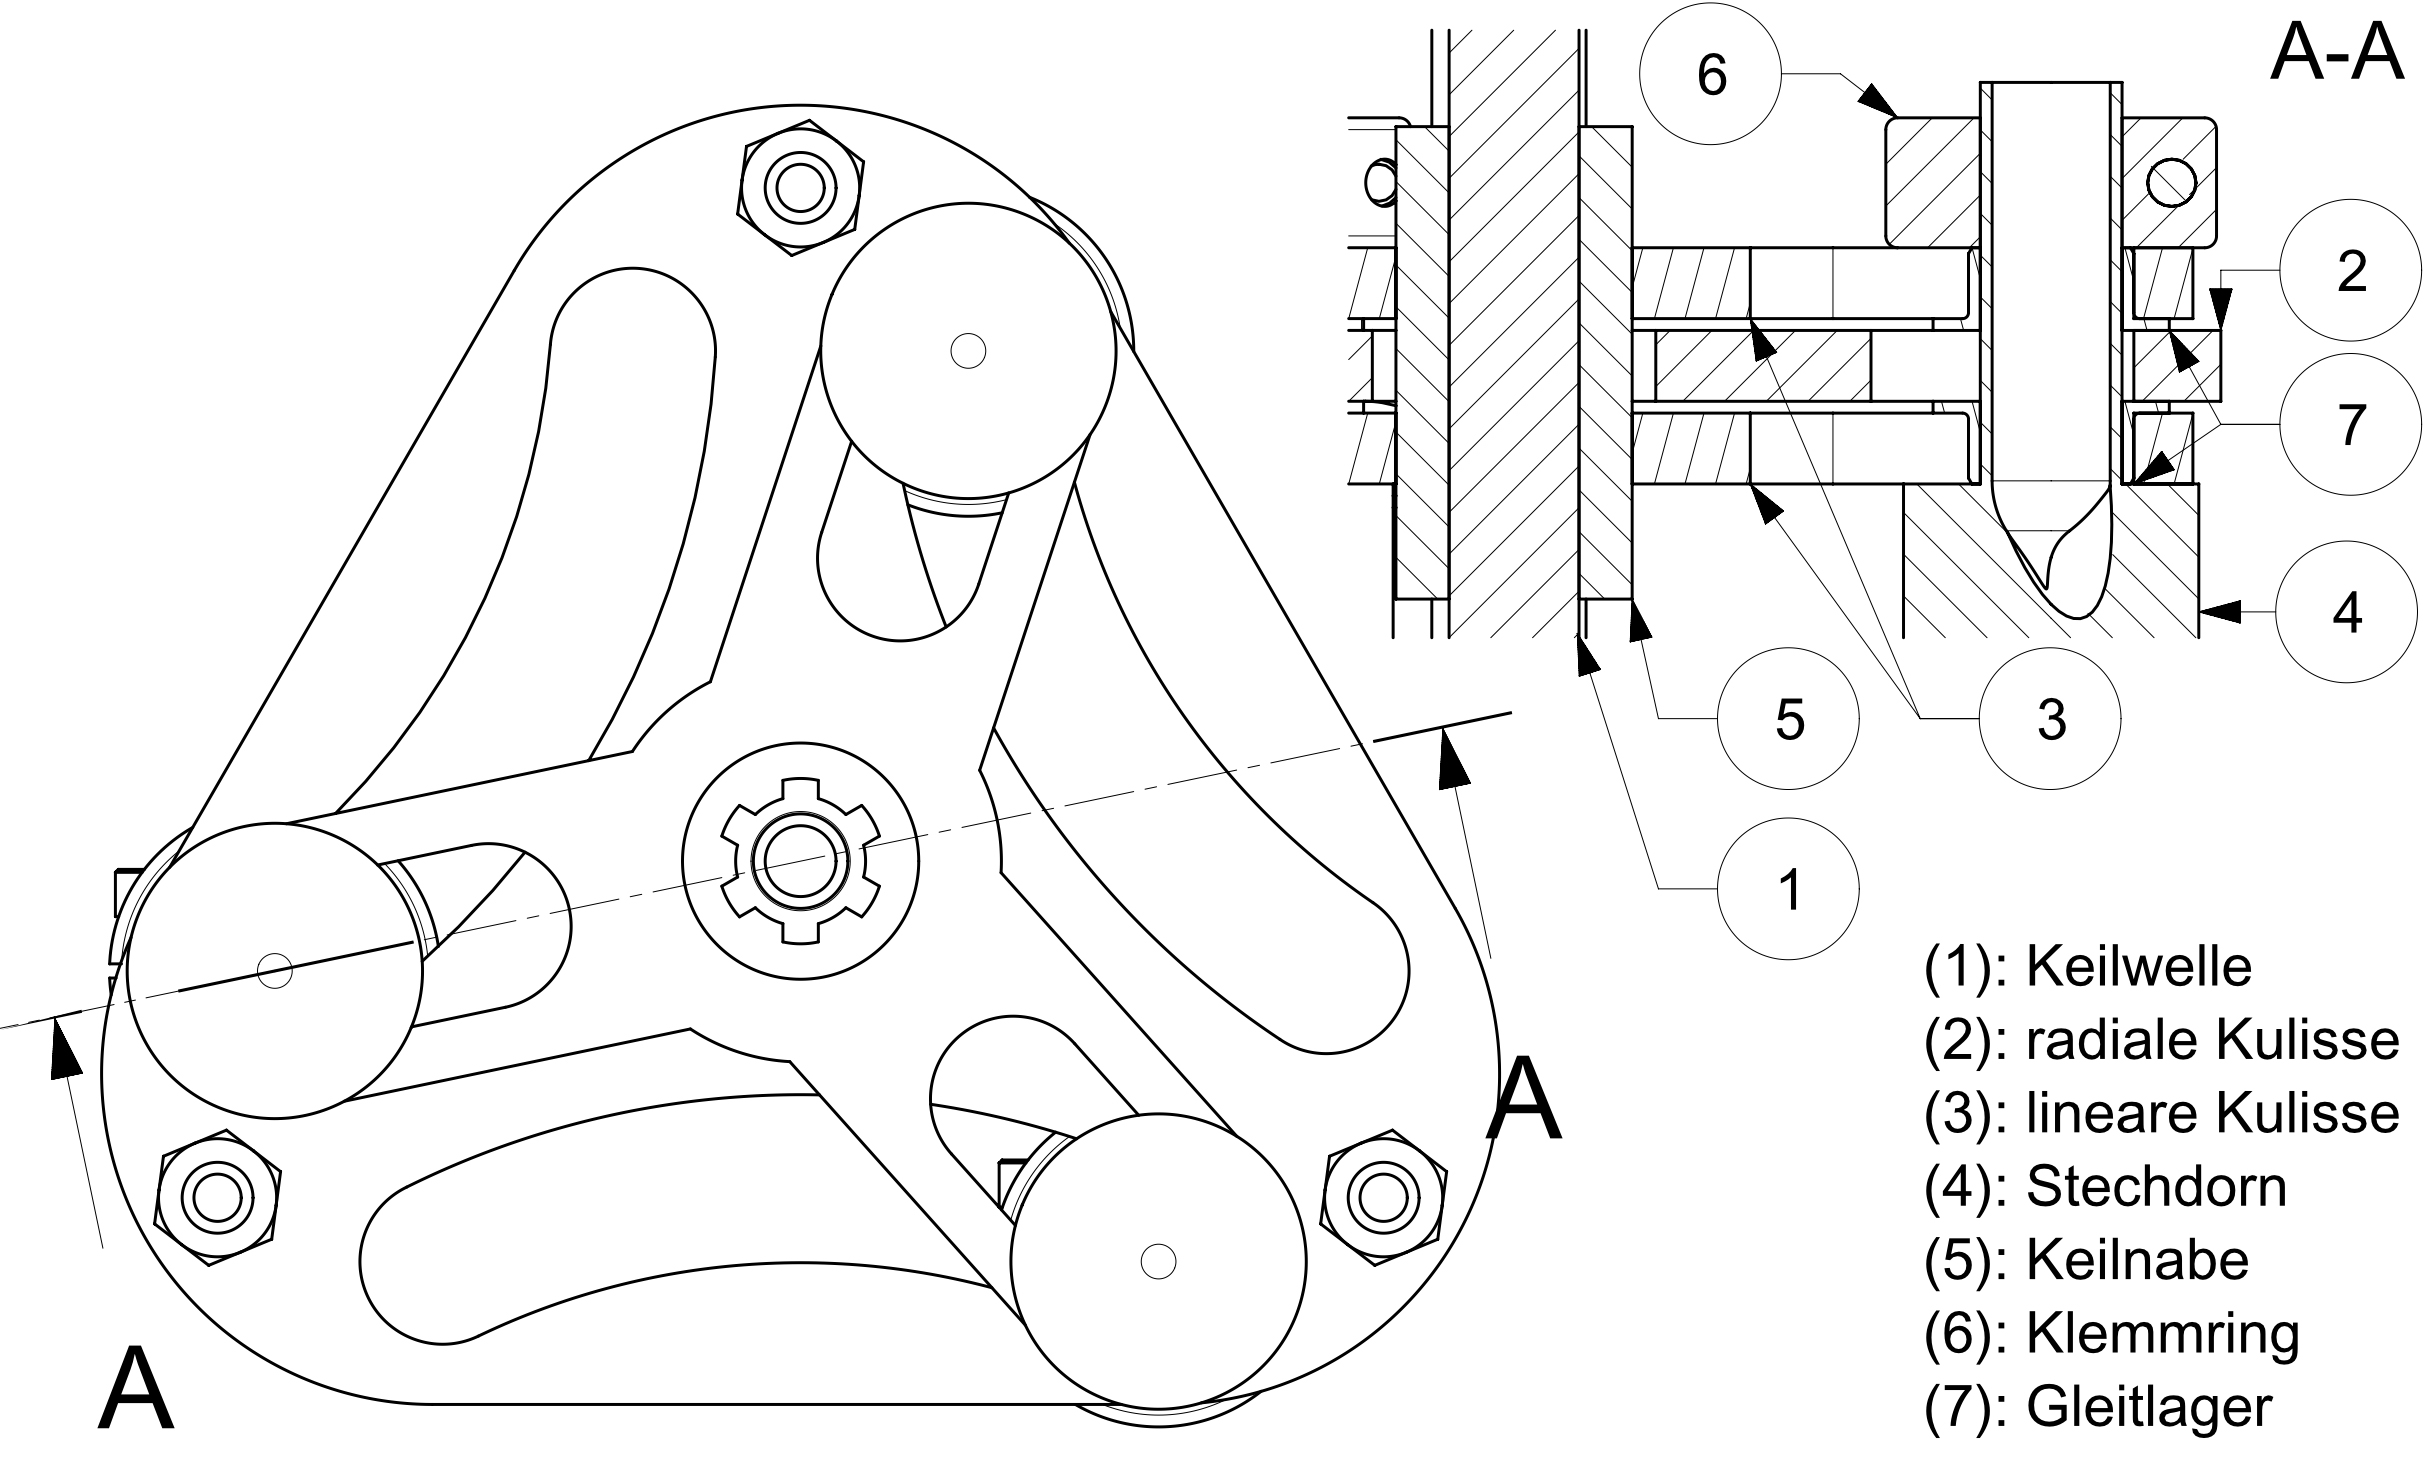
\includegraphics[scale=0.63]{Illustrationen/6-Umsetzung/schnitt_vm.jpg}
	\caption{Geschnittene Seitenansicht der Verstellmechanik}
	\label{fig:schnitt_vm}
	\end{figure}

\textbf{Funktion}
\newline
Die Bewegung der Verstellmechanik ist in Abbildung \ref{fig:motion_vm} dargestellt. Punkt B bildet ein beliebiger Punkt ab. So wird am Anschlag (Punkt A aus Abb. \ref{fig:motion_vm}) die Einsetzlokalität des grössten Topfes (Dmax = 140mm) und bei halbem Weg der Kulisse die Einsetzlokalität des kleinsten Topfes (Dmin = 90mm) erreicht. Dabei fällt auf, dass das Doppelte des nötigen Weges implementiert wurde. Begründet wird dies damit, dass dadurch der hochübersetzte Getriebemotor mehr Umdrehungen absolviert bis der gewünschte Radius erreicht wird. Dies steigert die Auflösung des Motors und verbessert die Regelbarkeit massiv.
	\begin{figure}[H]
	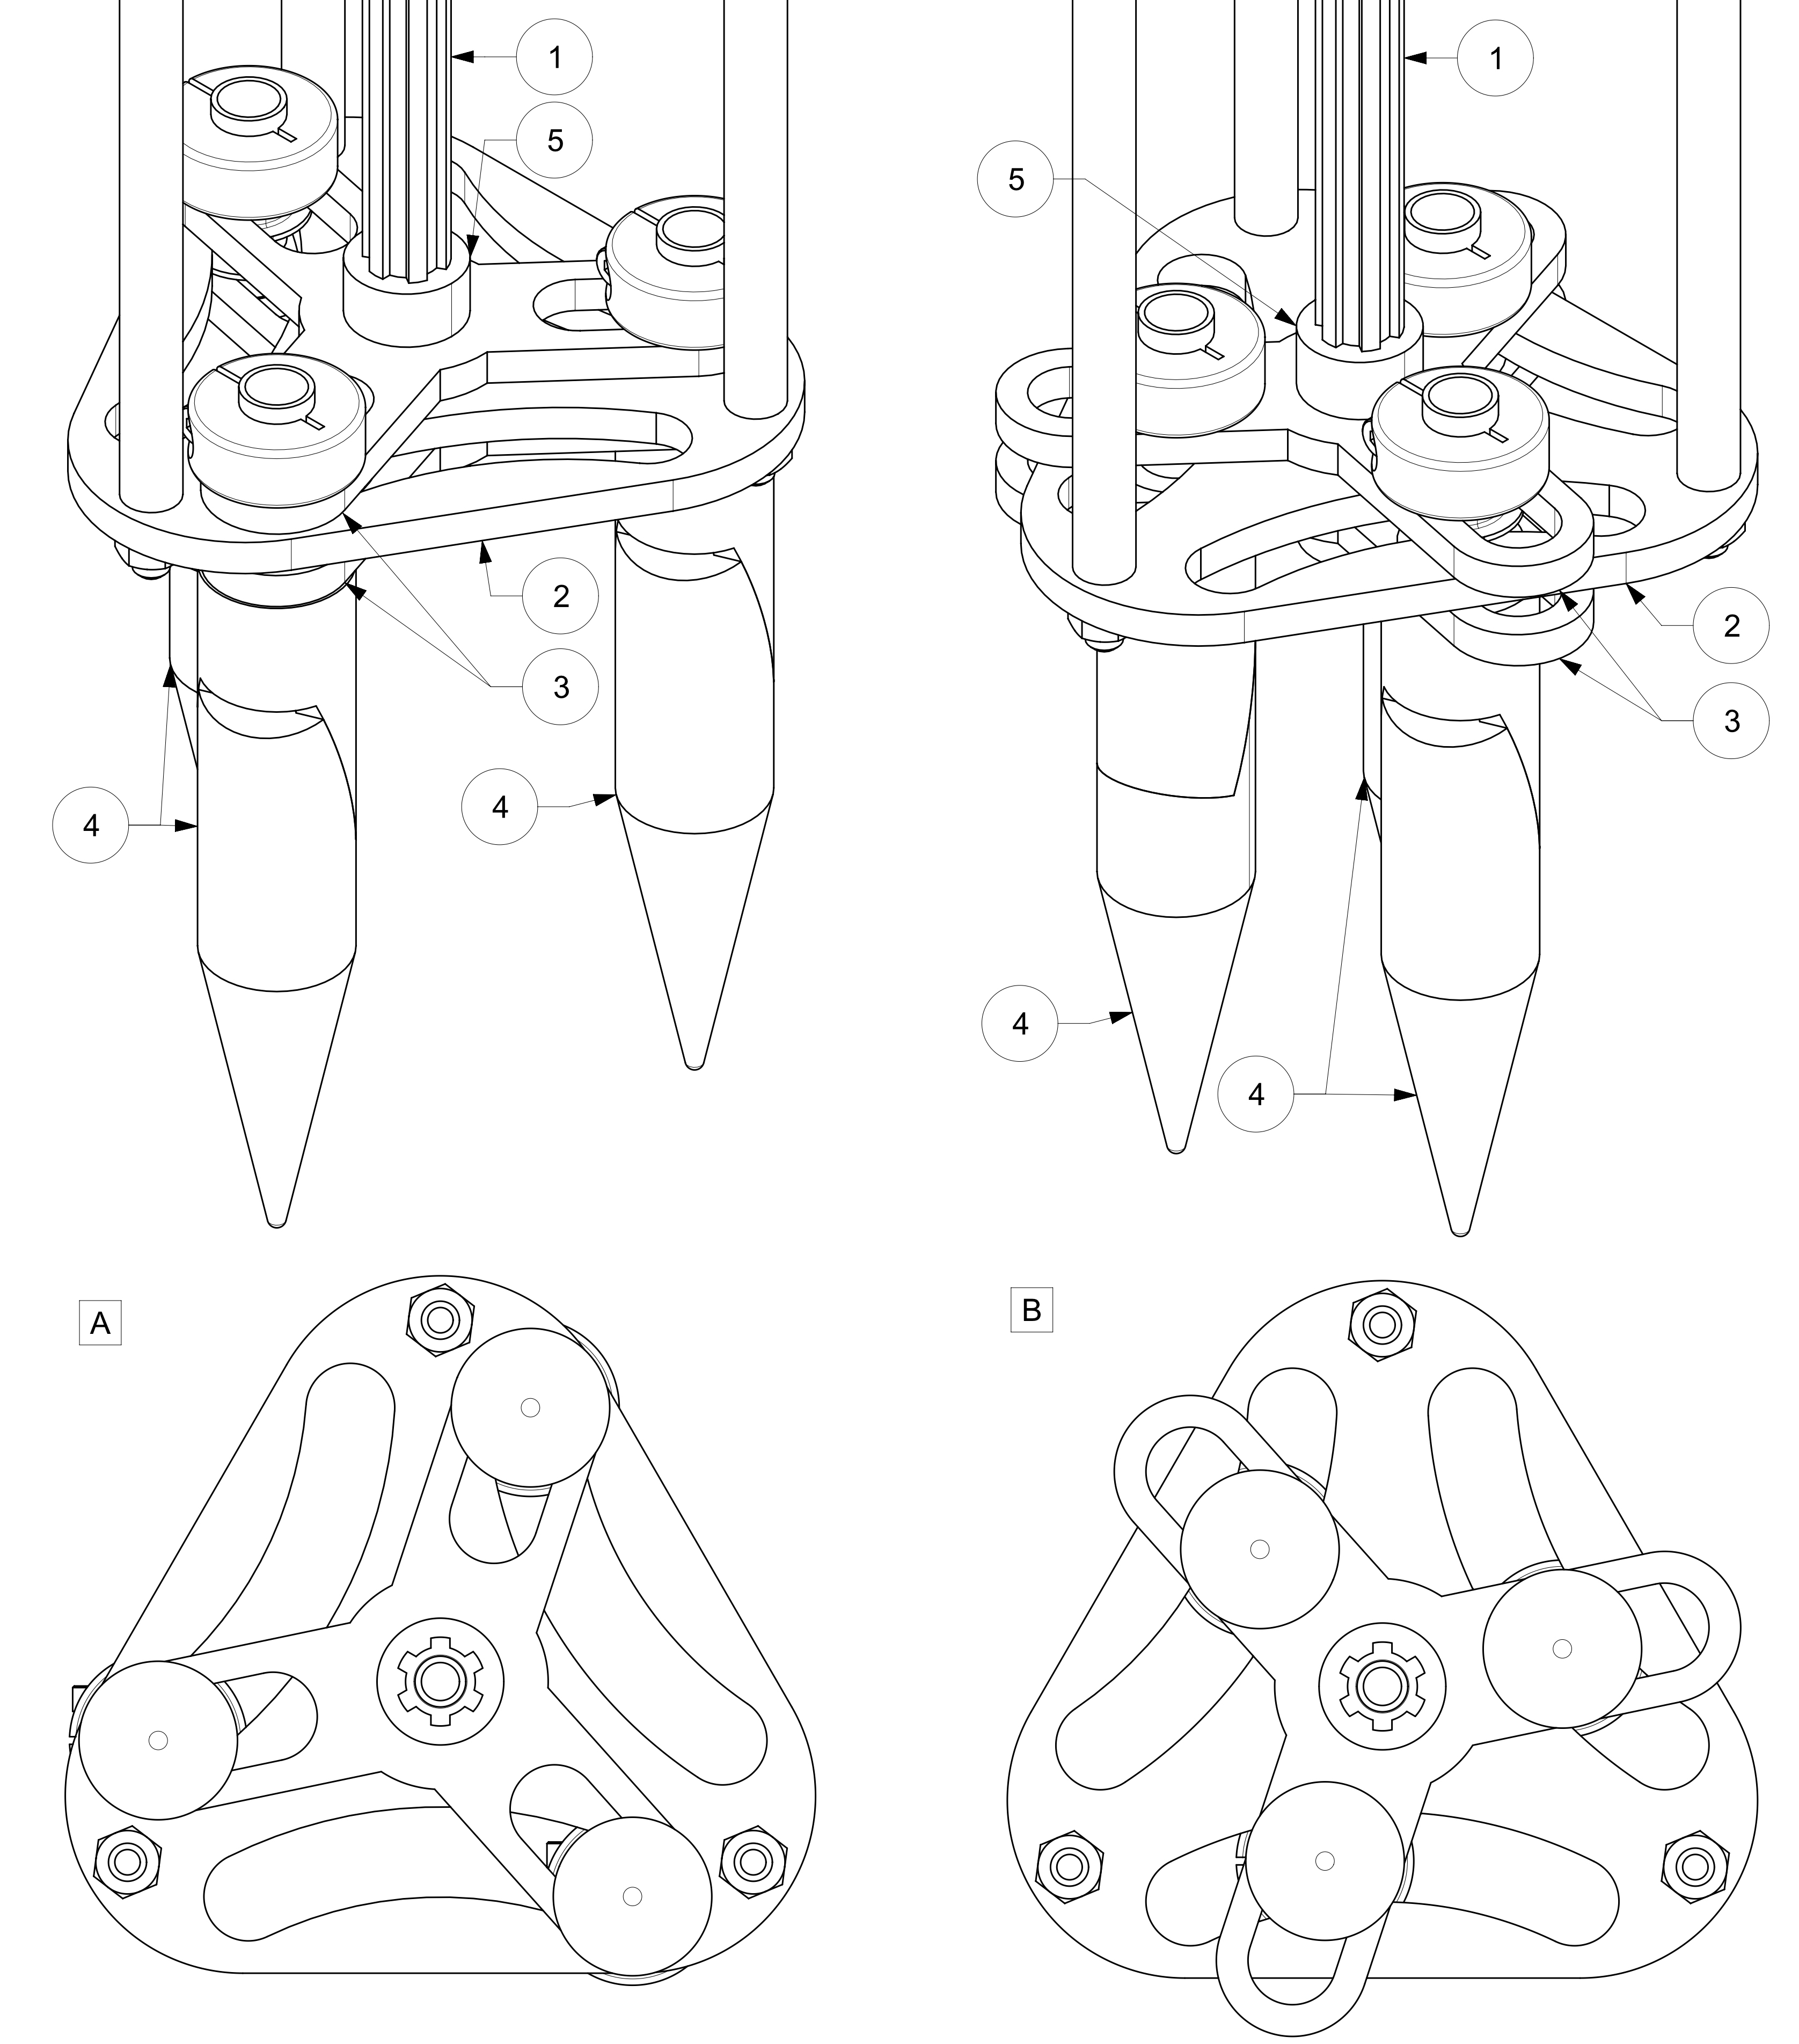
\includegraphics[scale=0.53]{Illustrationen/6-Umsetzung/motion_vm.jpg}
	\caption{Verstellung des Topfradius}
	\label{fig:motion_vm}
	\end{figure}
\textbf{Material und Fertigungsverfahren der Kulissen}
\newline
Wie schon erläutert, ist ein geringes Gewicht der beschleunigten Masse anzustreben. Gemäss Berechnungen soll die beschleunigte Masse maximal 1kg betragen. Um diese Anforderung zu erfüllen werden die Kulissen (Punkte 2 und 3 aus Abb. \ref{fig:motion_vm}) aus 6mm dickem Aluminiumblech gefertigt. So werden diese Teile auch mittels Laserschneidmaschine gefertigt. Weiter erspart diese Wahl das Umrüsten der Maschine und hält die Kosten auf einem Minimum (nochmals nötig?).
\subsection{Topferkennung}
\subsection{HMI}
\subsection{Peripherie}

\subsubsection{Maschinengestell}
\begin{wrapfigure}[16]{r}{6cm}
	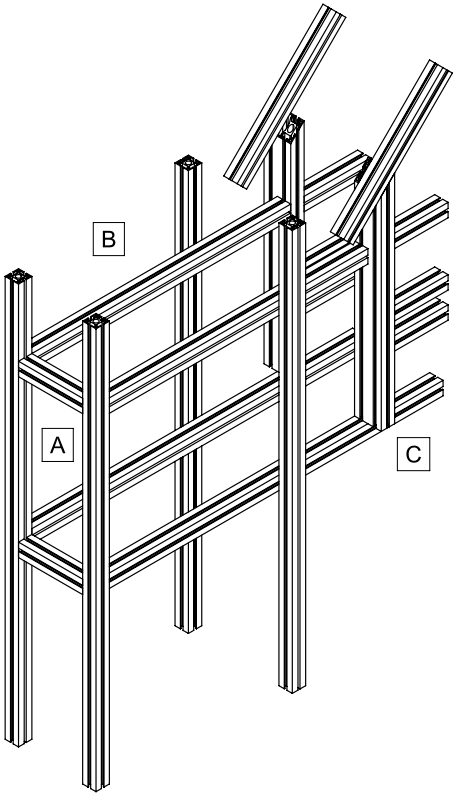
\includegraphics[scale=0.51]{Illustrationen/6-Umsetzung/maschinengestell.PNG}
	\caption{Maschinengestell}
	\label{fig:maschinengestell}
\end{wrapfigure}

Das Maschinengestell basiert auf dem Baukasten System von Kanya AG. Die Profile von Kanya AG eignen sich aus folgenden Gründen:
\begin{itemize}
	\item Dieses System ist einfach im Aufbau und der Montage. Das Maschinengestell ist so aufgebaut, dass eine Anpassung der Höhe (Punkt B in Abbildung \ref{fig:maschinengestell}) und die überstehende Länge der Setzeinheit (C) möglich ist. Diese Flexibilität wird durch die Verwendung der Universallverbinder von Kanya AG möglich.
	
	\item Das Profil hat an jeder Seite eine Längsnut. Dies bietet eine simple Lösung zur Montage der Montagebleche der Setzeinheit sowie Vereinzelung. Zudem ist im hinteren Teil des Gestells (A) eine Aluminiumplatte zur Montage der Elektronik vorgesehen.
	
	\item Die Tatsache, dass die Hochschule Luzern bei Kanya AG bereits Kunde ist, hebt Kanya AG von anderen Konkurrenten ab. Die positiven Erfahrungen und raschen Lieferzeiten überzeugen.
\end{itemize}


\subsubsection{Verdrahtung}

\subsection{Mainboard PCB}

\subsection{Vereinzelung} \label{sec:Inbetriebnahme_Vereinzelung}
spiel Pololu motor, Borstenlänge und Reibung erwähnen.

\begin{figure}[H]
	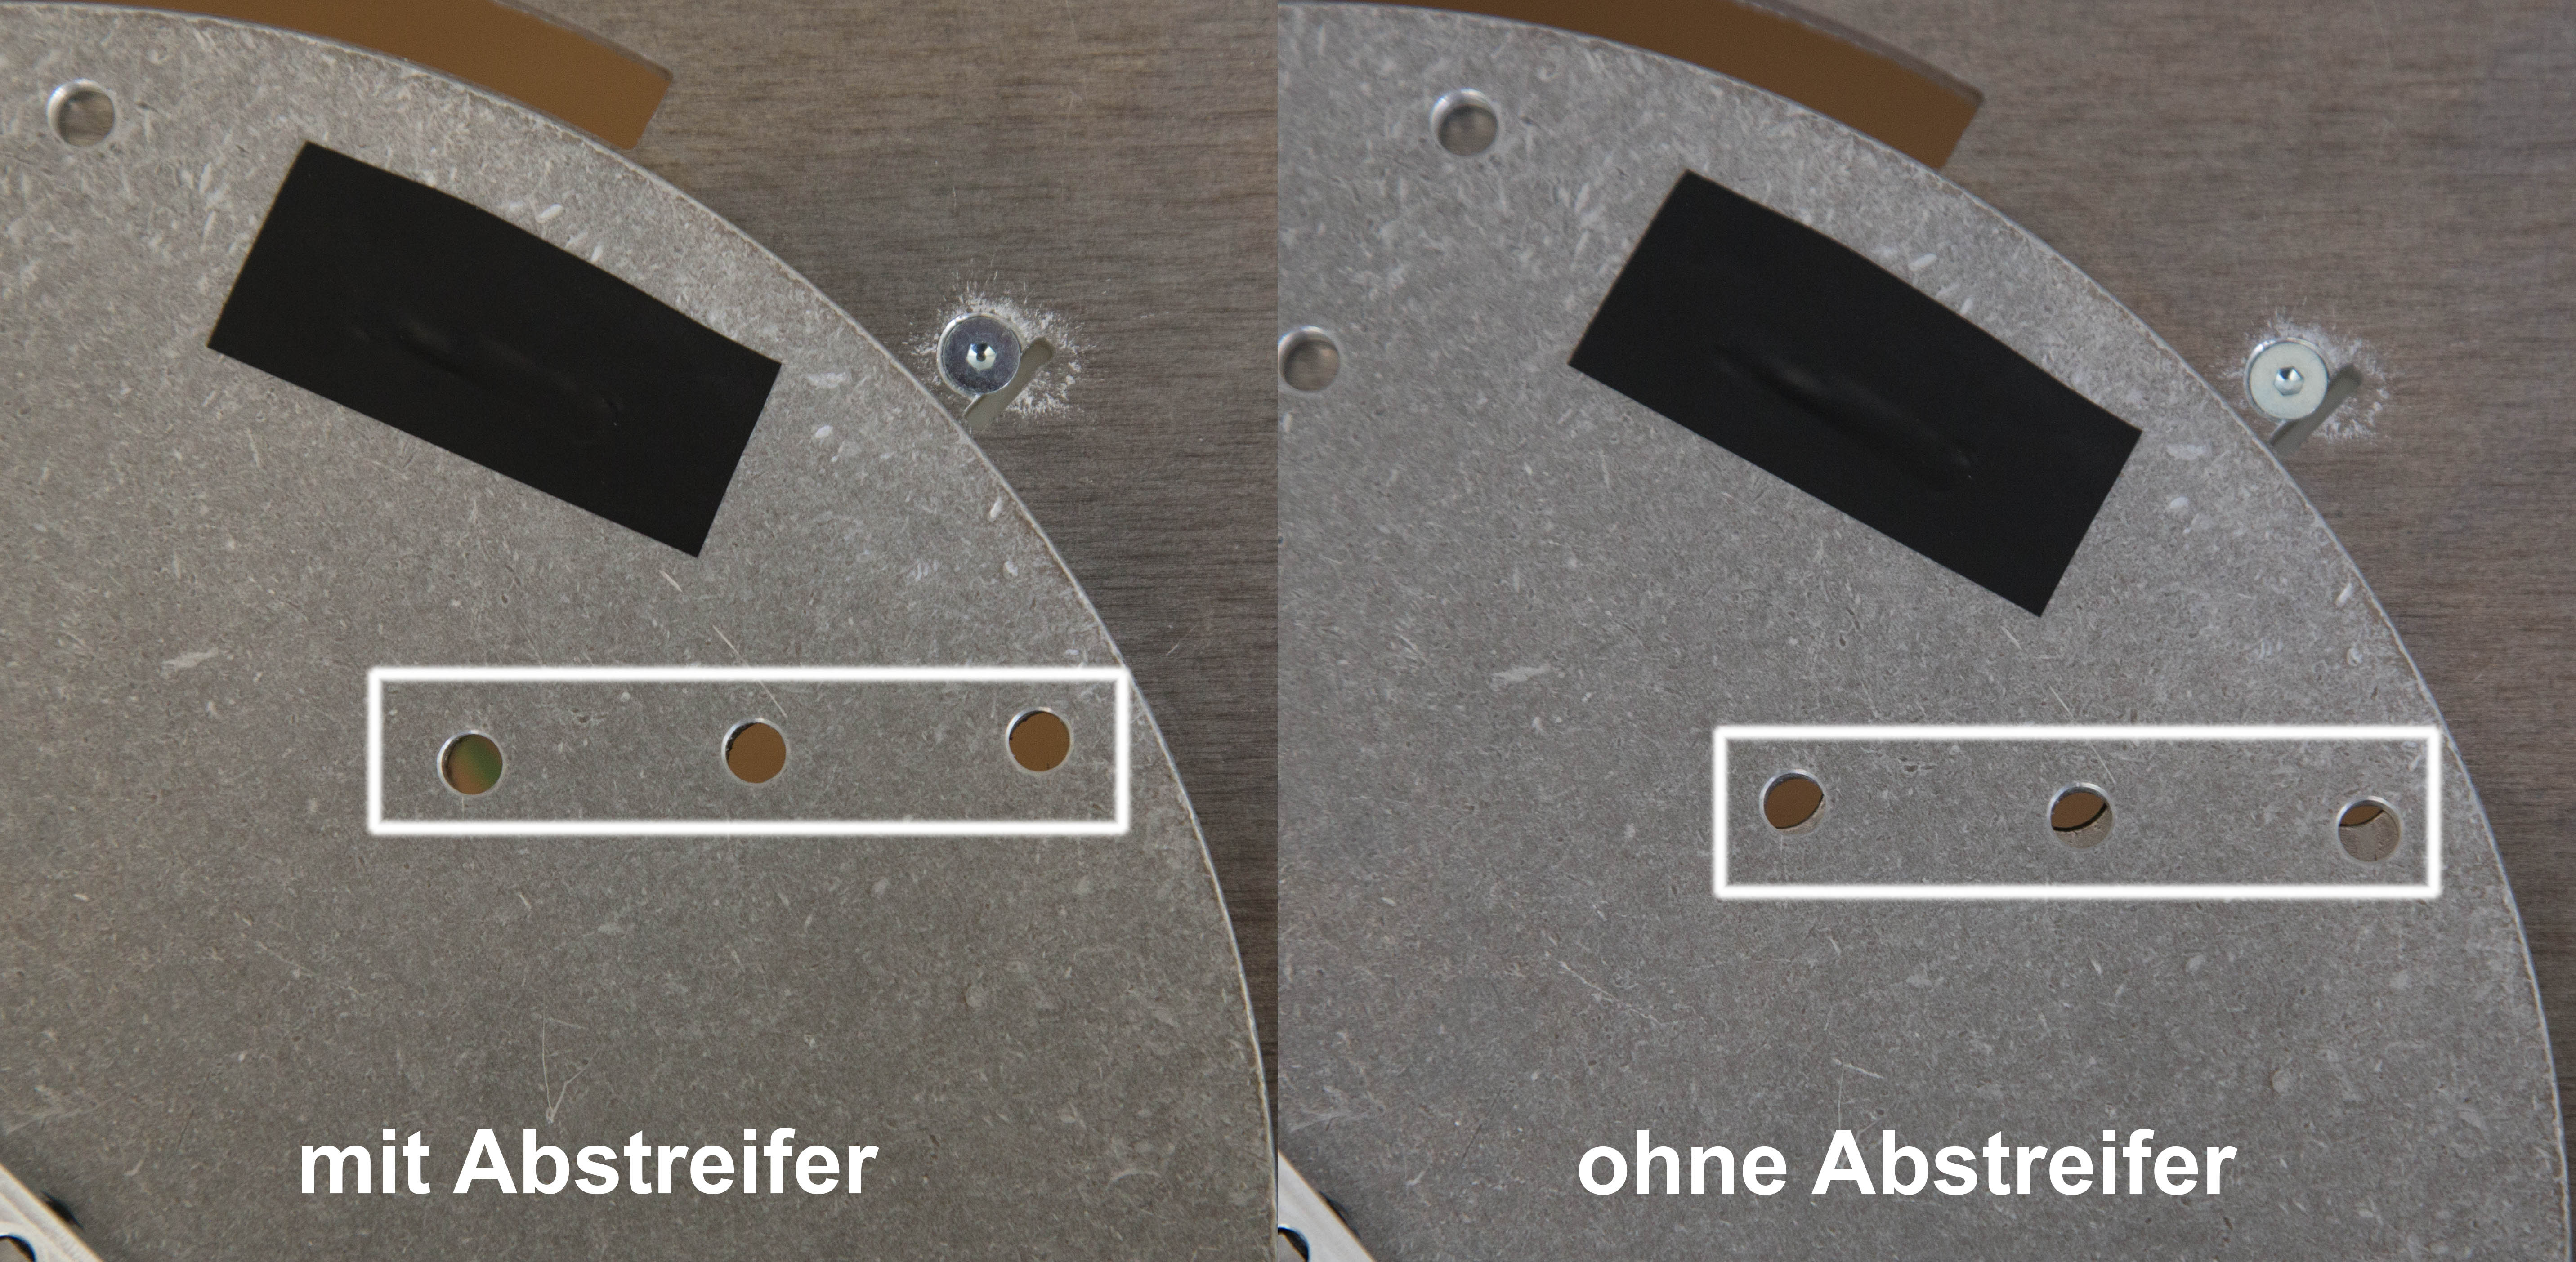
\includegraphics[width=1\textwidth]{Illustrationen/7-Inbetriebnahme_und_Kalibration/spiel_lochmaske.jpg}
	\caption{Spiel der Lochmaske mit und ohne Abstreifer}
	\label{fig:spiel_lochmaske}
\end{figure}
\subsection{Setzeinheit}
\subsection{Verstellmechanik} \label{sec:Inbetriebnahme_Verstellmechanik}
\textit{(pro)} Weil der für diese Anwendung evaluierte Motor für die Vereinzelung verwendet wurde, wurde hier der Motor mit der kleineren 1:100 Getriebeübersetzung und der höheren Leistung verwendet. Da die Stellgenauigkeit bei dieser Funktion gegenüber der Vereinzelung nicht so kritisch ist, kann der Motorentausch vertreten werden. Die Parametrisierung wurde experimentell ermittelt. Dazu wurde die Einheit von Anschlag zu Anschlag bewegt und die Anzahl Encoder Counts ausgelesen. Die Anzahl der ganzen Bewegung wurde dann linear auf 5 Position, stellvertretend für die 5 verschiedenen Topfgrössen, aufgeteilt. 

\begin{figure}[H]
	
\includegraphics[width=1\textwidth]{Illustrationen/7-Inbetriebnahme_und_Kalibration/verstellmechanik_1.jpg}
	\caption{verstellmechanik}
	\label{fig:verstellmechanik}
\end{figure}

Die Verstellmechanik kann durch diese Parametrisierung vorgeführt werden, die einstellbaren Topfgrössen entsprechen jedoch nicht den genauen Massen der verschiedenen Töpfen. In Abb. \ref{fig:verstellmechanik} sind vier verschiedene Stechradien A... D abgebildet welche durch Tastendruck auf dem HMI eingestellt werden können.
\newline
Die Verstellmechanik funktioniert somit prinzipiell einwandfrei und erfüllt die Anforderungen des Pflichtenheftes.
\subsection{Offene Punkte}
\textit{(pro)} In diesem Unterkapitel sind Punkte aufgeführt welche zur voll umfänglichen Erfüllung des Pflichtenhefts noch erledigt werden müssten (todo), sowie Punkte welche die Performance und Handhabung des Planting Robots verbessern würden (nice to have). 
\newline

\textbf{todo:}
\begin{itemize}
	\item Die Parameter der Verstellmechanik müssten gemäss den verschiedenen Setzradien ermittelt und in der Software geändert werden.
	\item Die Software müsste um eine adäquate Topferkennung erweitert werden. Die Sensoranbindung für einen IR-Sensor ist dabei schon implementiert.
	\item Entsprechend der Topferkennung müsste die FSM erweitert werden, sodass der Setzprozess bei erkanntem Topf ausgelöst wird.
	\item Das Gesamtsystem müsste als solches getestet werden. Dabei müssten Blumentöpfe angefüllt mit Topferde vom Planting Robot mit Nemacaps besetzt werden.
\end{itemize}

\textbf{nice to have:}
\begin{itemize}
	\item Die verwendeten PID Positionierungsregler für die Setzeinheit, Verstellmechanik und Setzeinheit könnten optimiert werden. Dafür müssten die Sprungantworten der jeweiligen Strecken ermittelt und über ein entsprechendes mathematisches Modell approximiert werden. Auf Grundlage der Strecke könnten dann die Parameter für den Regler definiert werden.
	\item Die Initialisierung der Setzeinheit könnte erweitert werden, indem die Setzeinheit nach erreichen des oberen Endanschlags bis an den unteren Anschlag fährt. Die dabei zurückgelegte Strecke könnte mit der tatsächlichen Länge der Spindel verglichen werden. Durch diesen Vergleich würde sichergestellt, dass die Setzeinheit nicht durch äussere Einflüsse (wie eine verschmutzte Spindel) fälschlicherweise einen Endanschlag vermutet.
\end{itemize}


\newpage
\section{Fazit}
\textit{(ygu)} Dieses Kapitel befasst sich mit der Verifikation des umgesetzten Funktionsmusters. Eine objektive Beurteilung der gesetzten Ziele wird gemacht. Dafür wird ein Vergleich mit dem zu Beginn verfassten Pflichtenheft angestellt. Weiter wird in diesem Kapitel auf alle offenen und unklaren Punkte eingegangen. Weiter werden konkrete Empfehlungen für den weiteren Verlauf dieses Projekts genannt.
\newline

Im zweiten Teil dieses Kapitels wird das Projektmanagement rückblickend betrachtet. Einen Soll-Ist-Vergleich betreffend Projektplan, Risikomanagement sowie Finanzierung wird gemacht.
\subsection{Zielbezug}
Der Zielbezug wird anhand des verfassten Pflichtenhefts durchgeführt. Die Orientierung am Pflichtenheft gewährleistet eine objektive Beurteilung der gesetzten Ziele. Dabei stützt sich die Beurteilung der einzelnen Ziele auf den gewonnen Erkenntnisse aus Kapitel \ref{inbetriebnahme}.
\newline

Die Verifikation der gesetzten Ziele ist in Tab. \ref{tab:verifikation} aufgelistet. Diese Tabelle bezieht sich auf das verfasste Pflichtenheft (vgl. Anhang: \textit{Pflichtenheft v1.6}). Dabei sind in dieser Tabelle alle relevanten Punkte für den Zielbezug zusammengefasst.

\begin{table}[H]
	\begin{tabular}{|L{0.5cm}|L{10.3 cm}|C{1.3cm}|C{2.3cm}|}
	\hline 
	\textbf{Nr.} & \textbf{Beschreibung} & \textbf{erfüllt?} & \textbf{Kommentar} \\ 
	\hline 
	1.2 &\textbf{Zielgruppe:} Gemüse- und Zierpflanzenbau. Töpfe mit Nenndurchmesser 
	90mm bis 140mm  & Ja & \\ 
	\hline 
	2.1 & \textbf{Abmessungen NemaCaps:} \newline 3mm (Durchmesser), +0.6mm  & Ja & Handhabung erfüllt \\ 
	\hline 
	2.2 & \textbf{Beschaffenheit NemaCaps:} \newline Elastisch, Widerstandsfähig & Ja & Handhabung erfüllt \\ 
	\hline 
	2.3 & \textbf{Handhabung:} In geschlossenem 
	Behälter unter Beigabe eines hygrophoben Pulver, ohne Zugabe von Wasser & Ja &  \\ 
	\hline 
	4.1 & \textbf{Aufbau Robot:} Stationär, auf Boden, an Topfmaschine fixiert & Ja &  \\ 
	\hline 
	4.2 & \textbf{Eingriffsort:} An Topfkranz, vor der Umleitung auf das 
	Förderband. & Ja &  \\ 
	\hline 
	4.3 & \textbf{Lagerung der NemaCaps:} Min. 10‘000 Stück Lagerkapazität, nicht länger als 1 Tag  & Ja &  \\ 
	\hline 
	4.4 & \textbf{Speisung:} 230V Netzspannung, max. Leistungsaufnahme 2kW & Ja &  \\ 
	\hline 
	4.5 & \textbf{Topferkennung:} Setzprozess soll nur ausgeführt werden, wenn sich 
	ein Topf auf dem Topfkranz befindet.  & unklar & Verifikation offen \\ 
	\hline 
				4.6 & \textbf{Topfkonfiguration (Fest):} \newline Der Planting Robot muss für jeden Batch mit der 
	Topfgrösse konfiguriert werden.  & Ja & Wunsch-anforderung umgesetzt \\ 
	\hline 
	\end{tabular} 

%	\caption{Verifikation der gesetzten Ziele durch das Pflichtenheft}
%	\label{tab:verifikation}
\end{table}	

\begin{table}[H]
	\begin{tabular}{|L{0.5cm}|L{10.3 cm}|C{1.3cm}|C{2.3cm}|}
		\hline 
		\textbf{Nr.} & \textbf{Beschreibung} & \textbf{erfüllt?} & \textbf{Kommentar} \\ 
		\hline 
		4.7 & \textbf{Topfkonfiguration (Wunsch):} Topfgrösse selbständig erkennen und dementsprechend konfigurieren.  & Ja & Konfiguration manuell möglich \\ 
\hline 
5.1 & \textbf{Einsetztiefe:} variabel, einstellbar. 
Maximale Einsetztiefe: 60\% der Topfhöhe & bedingt & nicht implementiert \\ 
\hline 
5.2 & \textbf{Bruchverhalten NemaCaps:} Dürfen nach Setzprozess beschädigt sein. Alle 
Bestandteile müssen sich in der Erde befinden.  & unklar & Verifikation offen \\ 
\hline 
5.3 & \textbf{Einsetzlokalität:} 3 Stück um den Mittelpunkt zu 120° versetzt, mit Durchmesser von 60\% des 
Topfdurchmessers, NemaCaps dürfen nicht durch das Loch für die Stecklinge 
eingesetzt werden.  & Ja &  \\ 
\hline 
5.4 & \textbf{Eingriffszeitpunkt:} Während Stopp Phase. Verhältnis 
Bewegungszeit/Eingriffszeit = 1:1. & unklar & Verifikation offen \\ 
\hline 
5.7 &  \textbf{Eingriffszeit 
	bei normaler Auslastung:} \newline 0.64s (2800 Töpfe/Stunde) & unklar & Verifikation offen \\ 
\hline 
5.8 &  \textbf{Eingriffszeit 
	bei maximaler Auslastung:} \newline 0.5s (3600 Töpfe/Stunde) & unklar & Verifikation offen \\ 
\hline 
\end{tabular} 
\caption{Verifikation der gesetzten Ziele durch das Pflichtenheft}
\label{tab:verifikation}
\end{table}	


Ergänzend ist hinzuzufügen:
\begin{itemize}

	\item Die Handhabung der NemaCaps (Punkte 2.1 und 2.2) ist mit dem umgesetzten Funktionsmuster gewährleistet. Für die erfolgreiche Handhabung ist es essentiell, dass ausschliesslich frische NemaCaps verwendet werden. 
	
	\item Die variable Einstellung der Einsetztiefe ist durch die Konstruktion sowie auch den Antrieb technisch möglich (Punkt 5.1). Die Implementation in der Software fehlt, wodurch dieser Punkt nur \textit{bedingt} erfüllt ist.
	
	\item Die Punkte 5.2, 5.4, 5.7 und 5.8 konnten nicht verfiziert werden, da für die Inbetriebnahme der Gesamtfunktion der zeitliche Rahmen fehlte. Da somit das Zusammenspiel der einzelnen Funktion nicht geprüft wurde, kann über diese Punkte keine Aussage gemacht werden.
	
	\item Die Topferkennung (Punkt 4.5) funktioniert prinzipiell. Durch die fehlende Zeit konnte die Implementation an der Topfmaschine (oder Testumgebung) nicht durchgeführt werden.
	
	\item Die Erfüllung von Punkt 4.6 ist obsolet, da die Wunschanforderung realisiert wurde.
	
	\item die selbständige Topfkonfiguration (Punkt 4.7) funktioniert. Die Kopplung mit der automatischen Topferkennung (Punkt 4.5) ist nicht implementiert, zurzeit muss die Konfiguration von einem Benutzer ausgelöst werden.
	
	\item Die Funktionen \textit{NemaCaps vereinzeln} und \textit{Setzmechanismus konfigurieren} funktionieren grundsätzlich. Da die formulierten Punkte im Pflichtenheft sich auf das ultimative Endresultat beziehen, haben diese Teilerfolge nur wenig Gewicht in der Verifikation.
\end{itemize}

Abschliessend wird befunden, dass alle Funktionen, die im zeitlichen Rahmen gestestet wurden, ihre Funktion erfüllen. Für alle anderen (nicht getesteten) kann zum jetzigen Zeitpunkt kein abschliessendes Urteil gemacht werden.
\input{Kapitel/8_Fazit/8.2_Rückblick}
\subsection{Massnahmen / Empfehlungen}

\newpage
\section{Schlusswort}

\textbf{Maschinentechnik - Yves Gubelmann}
\newline
\textit{(ygu)} Die Bachelorarbeit begleitete mich durch das sechste und letzte Semester im Studium Maschinentechnik an der Hochschule Luzern. Die erhaltene Aufgabenstellung schien mir zu Beginn leicht abstrakt und nur grob definiert. Die offene Formulierung der Aufgabenstellung liess uns einen grossen Gestaltungsfreiraum  zu und konfrontierte uns gleichzeitig mit Eigenverantwortung. Während der Entwurfsphase nahmen wir durch das Festlegen der Rahmenbedingungen eine aktive Rolle ein, was ich sehr schätzte. Der stetige Austausch mit dem Industriepartner und den betreuenden Dozenten führte in dieser Phase zu einem klaren Verständnis der Aufgabenstellung sowie Vorgehensweise.
\newline

Die Konzeptausarbeitung empfand ich als spannender Prozess während der gesamten Bachelorarbeit. Es entstanden unzählige interessante Lösungsansätze, welche nur im interdisziplinären Austausch mit meinem Arbeitskollegen möglich wurden. Die kreative Findung von innovativen Lösungen war bereichernd, jedoch auch entscheidend für den weiteren Verlauf dieser Arbeit. Nur eine sorgfältige Abwägung aller Kriterien gewährleistete eine pragmatische Wahl des Lösungskonzeptes.
\newline

Die Umsetzungsphase bleibt mir als intensiv und lernreich in Erinnerung. Die Konstruktion des Funktionsmusters stellte mich vor Herausforderungen, die für mich als gelernter Elektroniker unbekannt waren. Vor allem in den Bereichen des gerechten Einsatzes von Materialien und Fertigungsverfahren konnte ich neue Erfahrungen sammeln. Ich erkannte, wie wichtig die Zusammenarbeit im Team ist, um unnötigen Aufwand und allfällige Komplikationen zu vermeiden. Die anschliessende Realisierung des Funktionsmusters erwies sich als spannende Abwechslung zur computerlastigen Konstruktion. Unser Lösungsansatz konnte erfolgreich realisiert werden, was mir viel Freude bereitet und mir bestätigt, dass die intensive Arbeit in den vergangenen Monaten, sich gelohnt hat.
\newline

Mit dem Gesamtergebnis dieser Bachelorarbeit bin ich zufrieden, obwohl einzelne Teilfunktionen nicht wie geplant funktionieren. Die formulierten Massnahmen, welche das Funktionsmuster ergänzen sollen, stimmen mich optimistisch, dass der Pflanzroboter für den Einsatz bereit ist.
\newline

Rückblickend gefiel mir das vertiefte Arbeiten an einer Problemstellung und die selbständige Arbeitsweise sehr. Der straffe Zeitplan erforderte eine gute Planung und ein erhöhtes Mass an Eigendisziplin. Ich bin der Meinung, dass wir ein gutes Team bildeten und die Kommunikation miteinander funktionierte. Der kollegiale und respektvolle Umgang sehe ich dabei als zentrale Grundlage. Die frühzeitigen Erkenntnisse durch die Funktionsnachweise, erschient mir im Nachhinein als besonders zentral. Dadurch wurde gewährleistet, dass Probleme nicht erst am Funktionsmuster erkannt wurden, sondern bereits zu einem frühen Zeitpunkt.
\newline

Zufrieden und mit positiven Erfahrungen blicke ich auf eine intensive Bachelorarbeit zurück. Sie begleitete mich eng während dem Abschluss meines Studiums. Ich bin optimistisch, dass ich die gemachten Erfahrungen in der Industrie anwenden und davon profitieren kann.
\newline

\textbf{Elektrotechnik - Patrick Rossacher}
\newline
\textit{(pro)}
\newline	

\textbf{Danksagung}
\newline
\textit{(ygu/pro)} Zum Schluss möchten wir allen beteiligten Personen danken, welche uns während dieser Zeit unterstützt haben. Ein besonderer Dank geht an unseren betreuenden Dozenten, Markus Thalmann und Marco De Angelis. Dank Ihrer unkomplizierten und kompetenten Beratung waren Sie stets eine Hilfe. Auch möchten wir uns bei Herrn Jean-Antoine Meiners für die Ermöglichung dieser Bachelorarbeit bedanken. Das grosse Vertrauen das er in uns hatte und die stete Motivation, schätzten wir sehr.


\newpage

\bibliography{Quellen/literatur}
\newpage
\begin{appendix}
\section{Anhang}
Folgende Dokumente befinden sich in schriftlicher Form im Anhang:

\begin{itemize}
	\item \verb|Aufgabenstellung|
	\item \verb|Funktionsbezogene Variation|
	\item \verb|Morphologischer Kasten|	
	
\end{itemize}

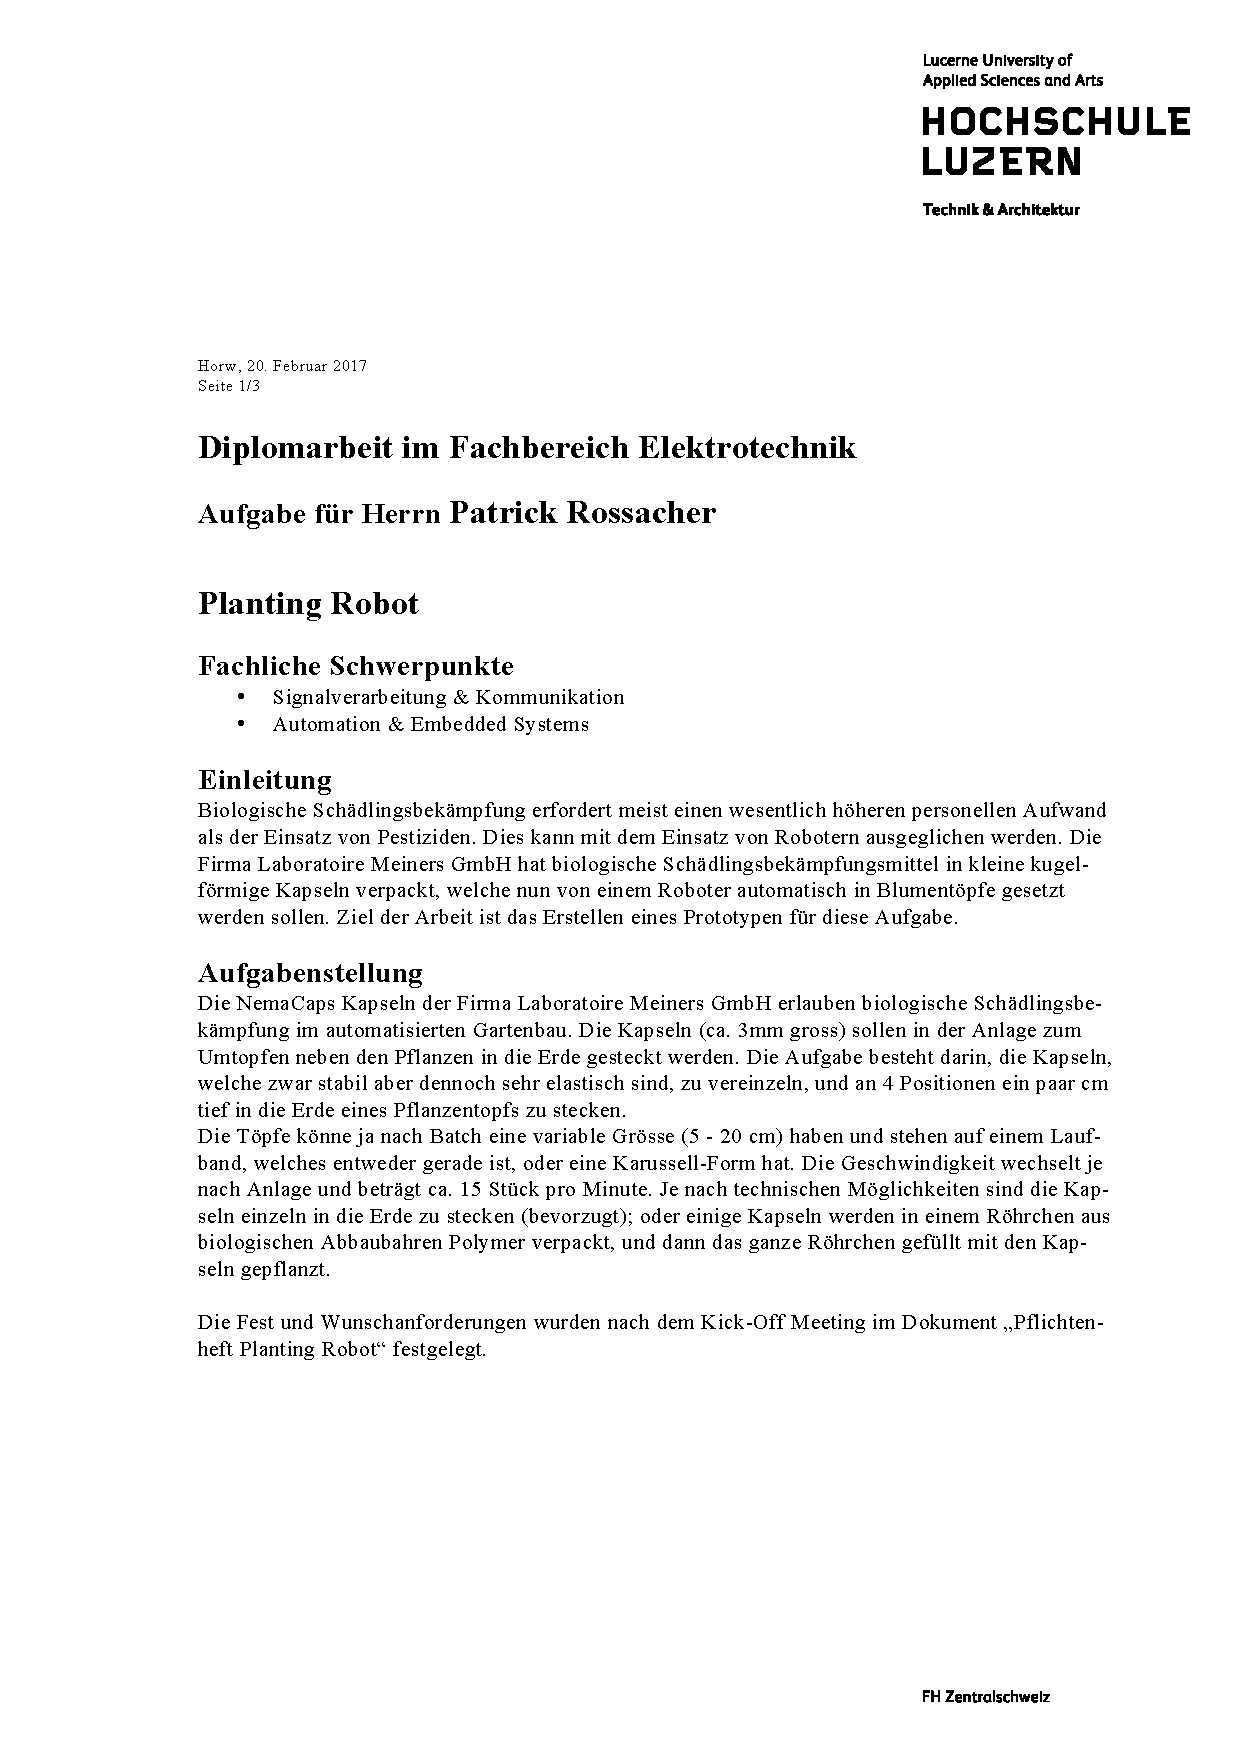
\includepdf[pages=-,nup=1x1]{Illustrationen/10-Anhang/Aufgabenstellung.pdf}
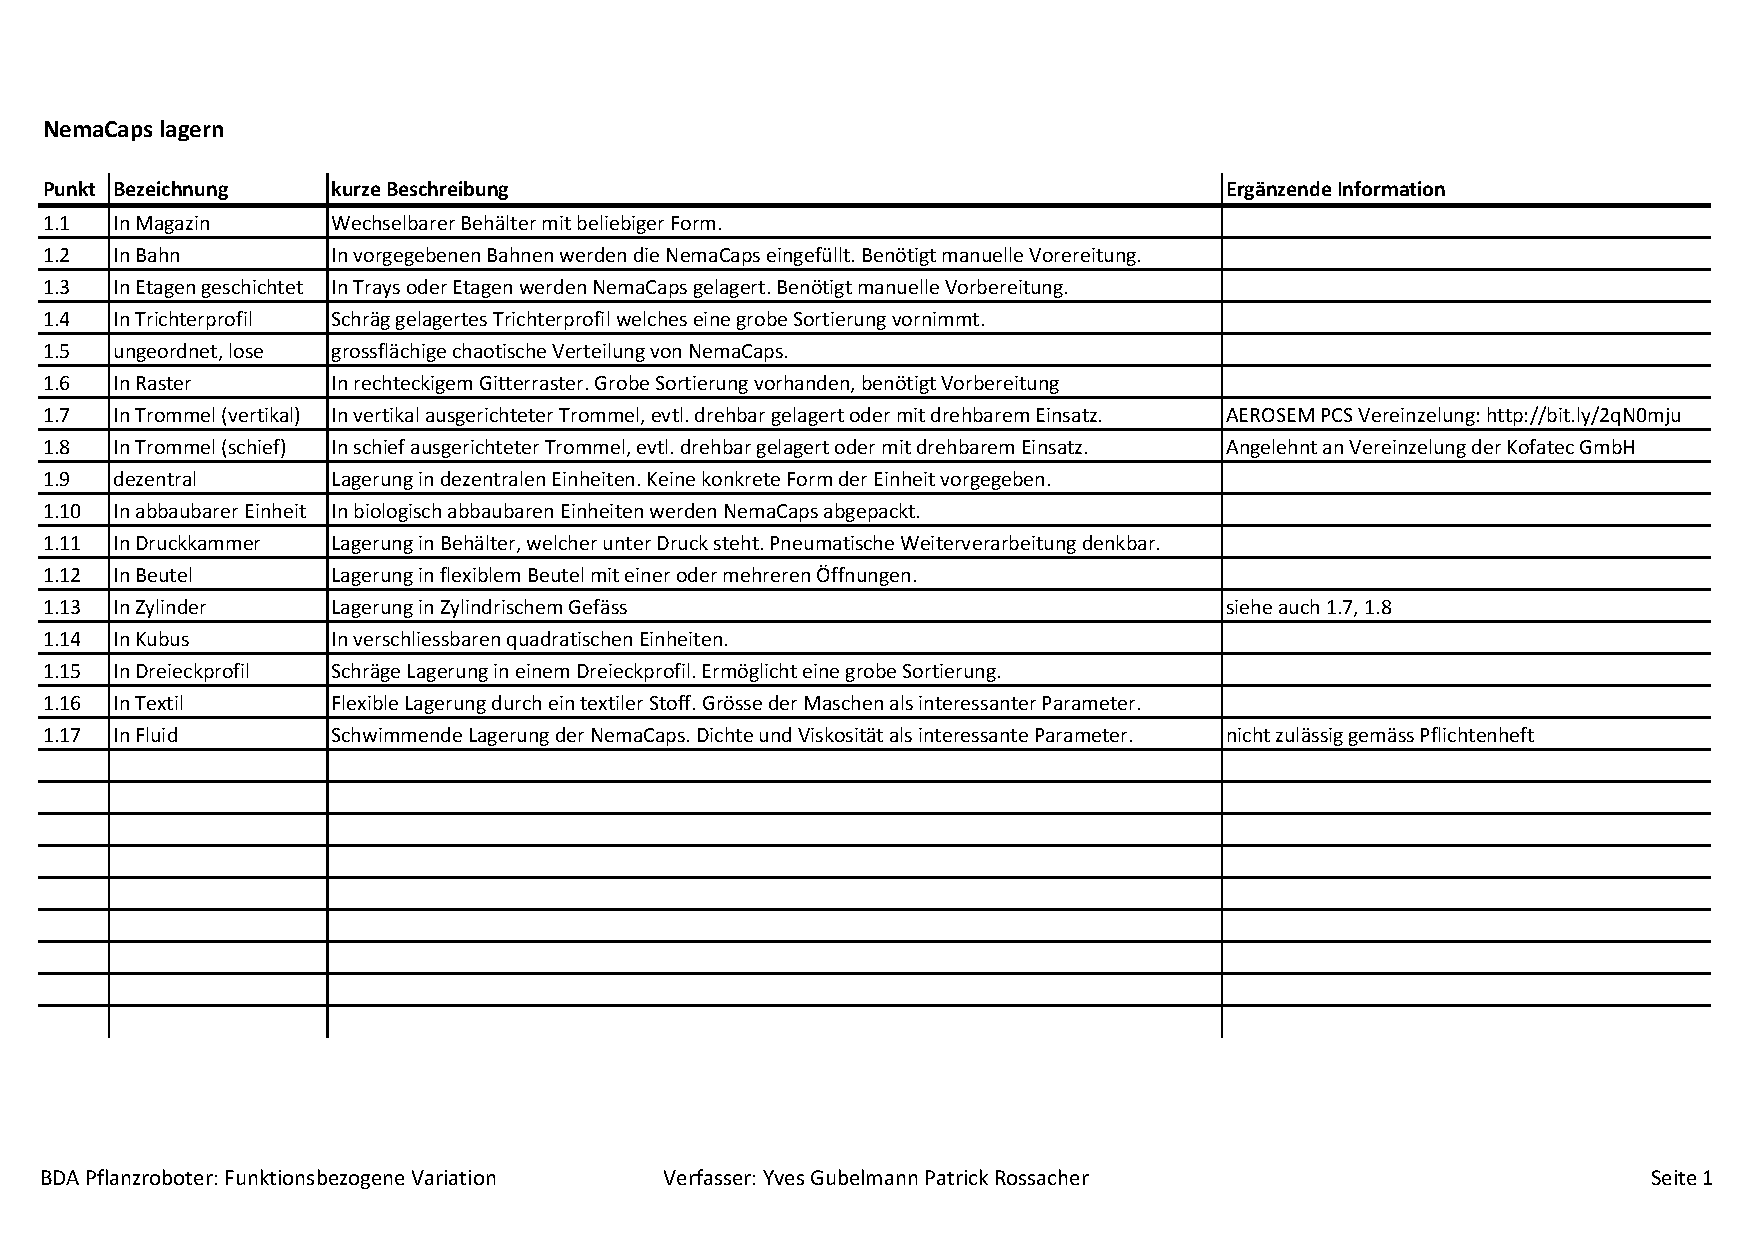
\includepdf[pages=-,nup=1x1]{Illustrationen/10-Anhang/Funktionsbezogene_Variation.pdf}
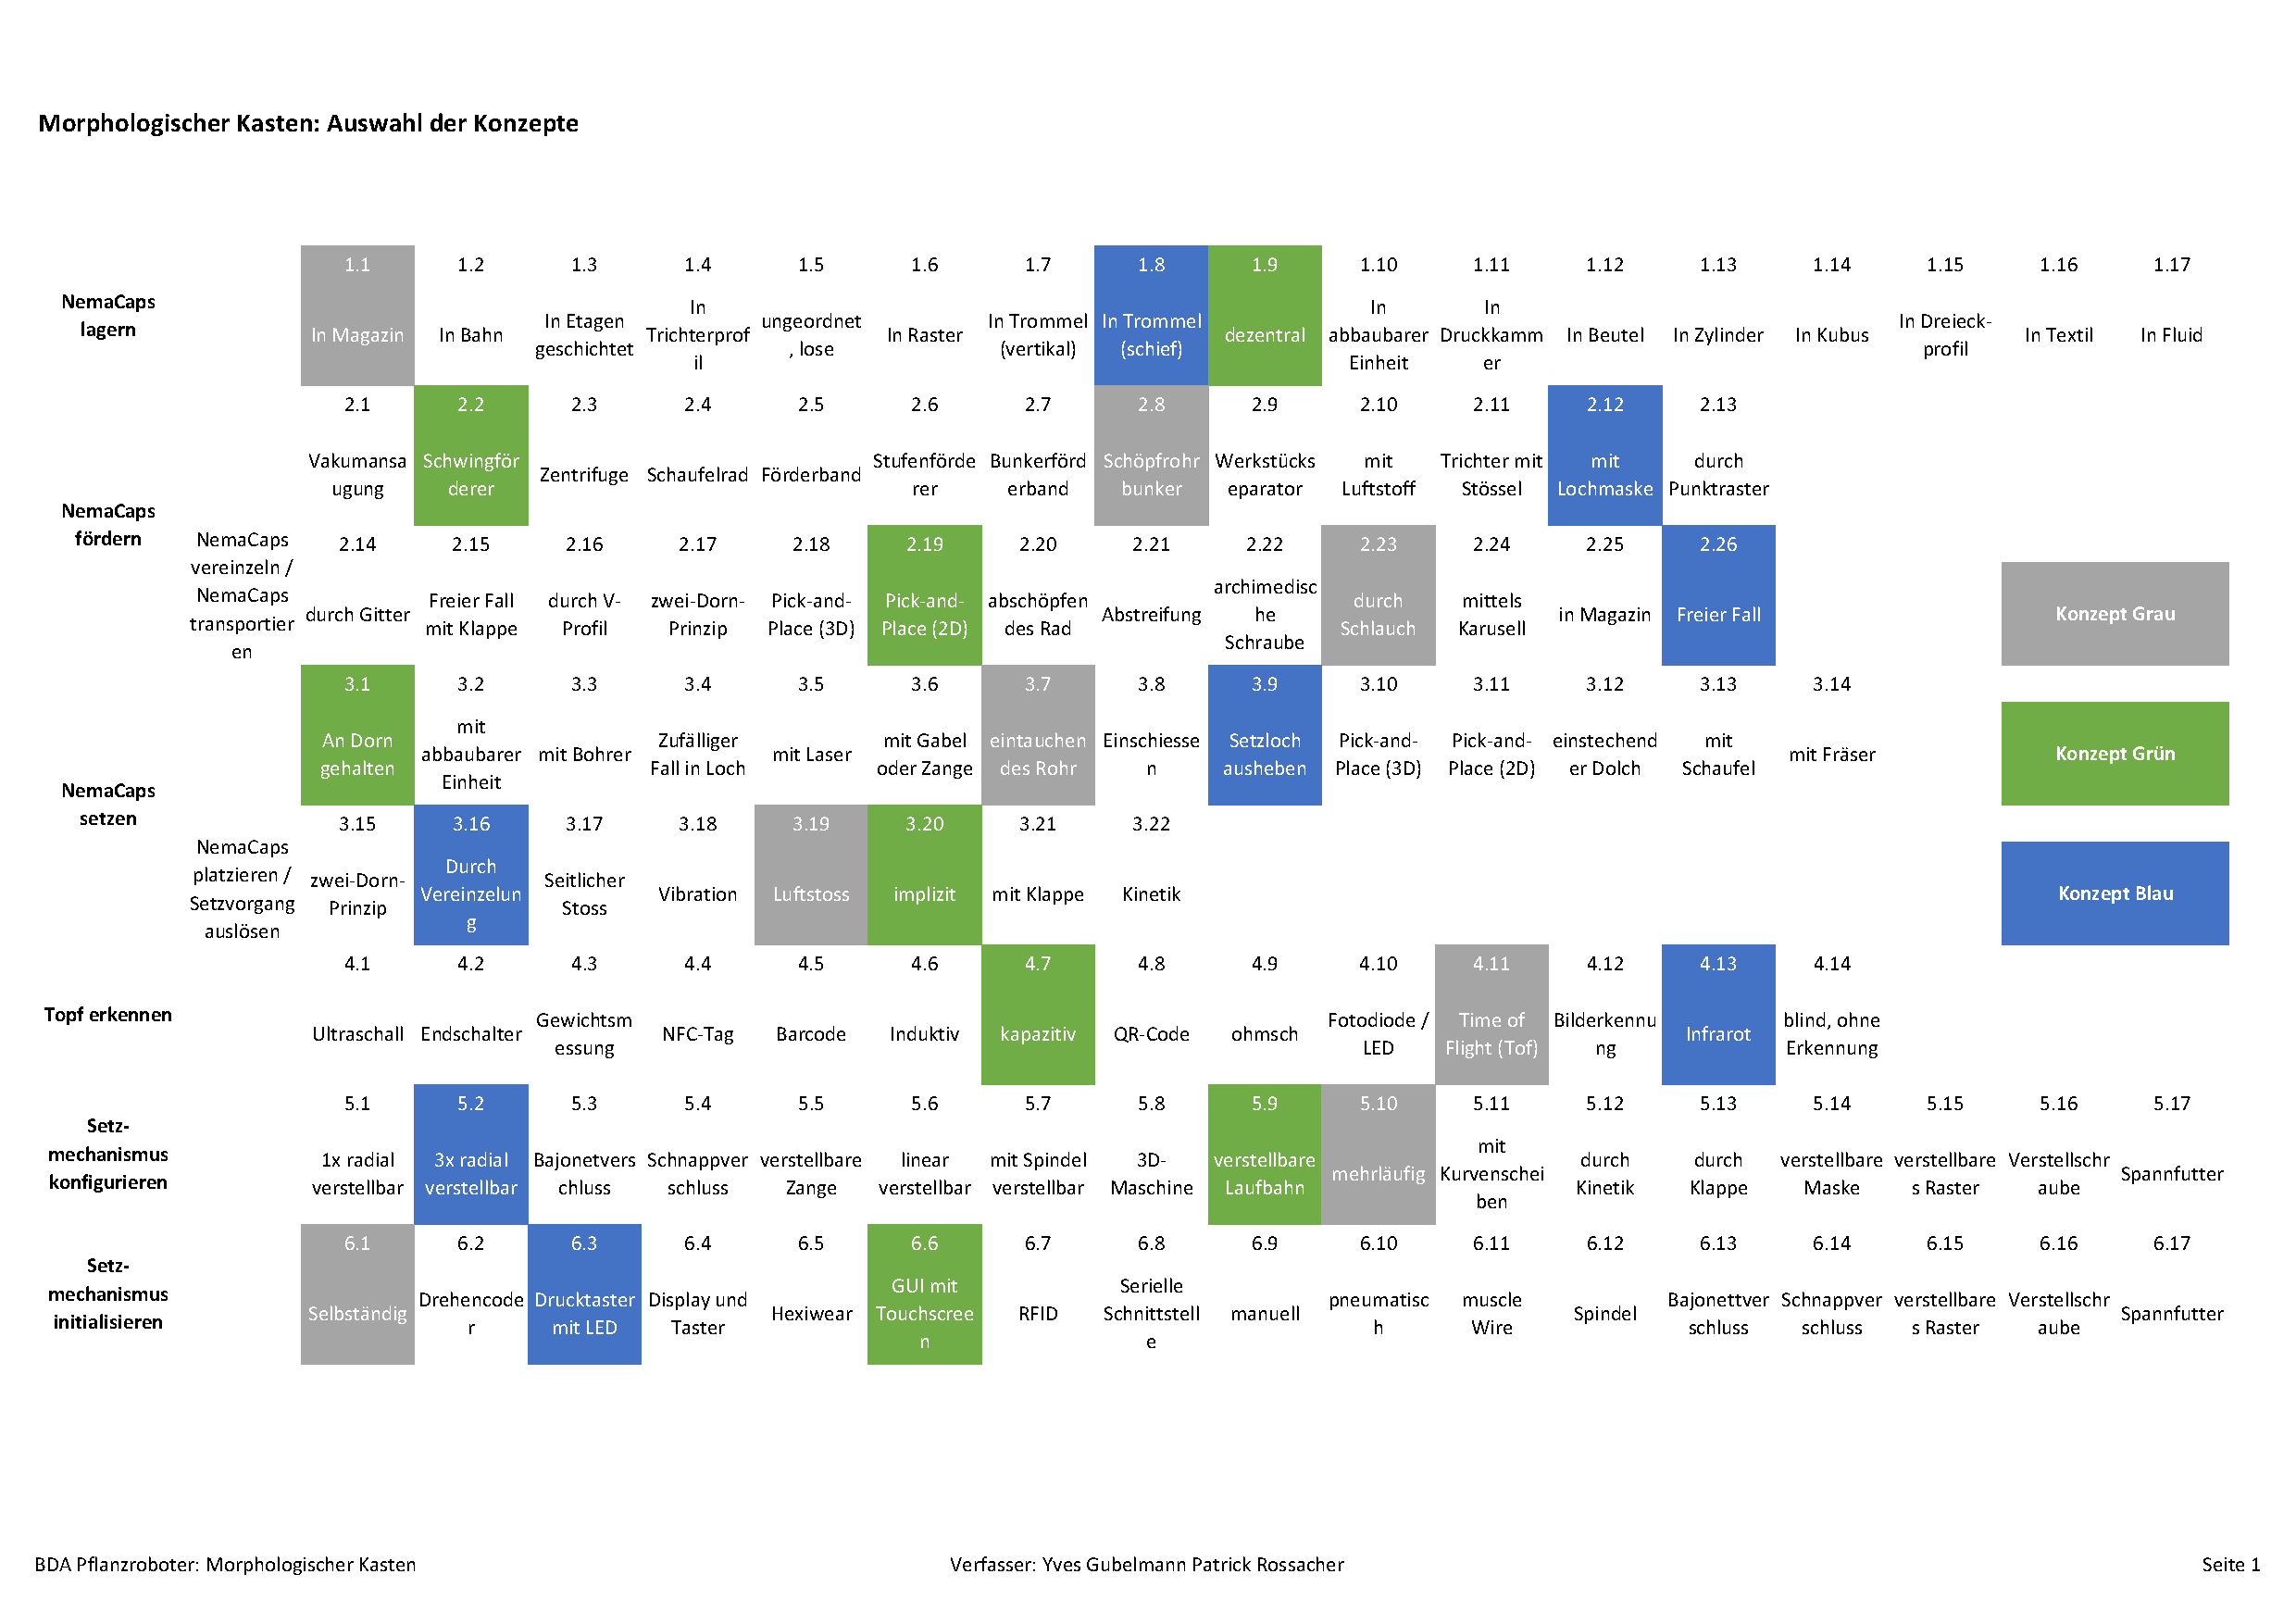
\includepdf[pages=-,nup=1x1]{Illustrationen/10-Anhang/Morphologischer_Kasten.pdf}

\end{appendix}
\end{document}